\documentclass{article}

\usepackage{makeidx}
\usepackage{latexsym}
\usepackage{moreverb}
\usepackage{index}
\usepackage{subfigure}
\usepackage{boxedminipage}
\usepackage{fancybox}
\usepackage{fancyhdr}


\usepackage{ifpdf}
\newif\ifpdf
\ifx\pdfoutput\undefined
\else
  \ifx\pdfoutput\relax
  \else
    \ifcase\pdfoutput
    \else
      \pdftrue
    \fi
  \fi
\fi
\ifpdf
  \usepackage[pdftex,colorlinks=true,bookmarksopen, pdfstartview=FitH,
              linkcolor=blue, citecolor=blue, urlcolor=blue]{hyperref}
  \usepackage[pdftex]{graphicx}
  \pdfcompresslevel=9
\else
  \usepackage[dvips]{graphicx}
\fi


% ----------------------------------------------------------------
% HORIZONTAL MARGINS
% Left margin, odd pages: 1.25 inch (0.25 + 1)
\setlength{\oddsidemargin}{0.25in}
% Left margin, even pages: 1.25 inch (0 + 1)
\setlength{\evensidemargin}{0.25in}
% Text width 6 inch (so other margin is 1.25 inch).
\setlength{\textwidth}{6in}
% ----------------
% VERTICAL MARGINS
% Top margin 0.5 inch (-0.5 + 1)
\setlength{\topmargin}{-0.5in}
% Head height 0.25 inch (where page headers go)
\setlength{\headheight}{0.25in}
% Head separation 0.25 inch (between header and top line of text)
\setlength{\headsep}{0.25in}
% Text height 9 inch (so bottom margin 1 in)
\setlength{\textheight}{9in}
% ----------------
% PARAGRAPH INDENTATION
\setlength{\parindent}{0in}
% SPACE BETWEEN PARAGRAPHS
\setlength{\parskip}{\medskipamount}
% ----------------
% EMPTY BOXES OF VARIOUS WIDTHS, FOR INDENTATION
\newcommand{\hm}{\hspace*{1em}}
\newcommand{\hmm}{\hspace*{2em}}
\newcommand{\hmmm}{\hspace*{3em}}
\newcommand{\hmmmm}{\hspace*{4em}}
% ----------------
% VARIOUS CONVENIENT WIDTHS RELATIVE TO THE TEXT WIDTH, FOR BOXES.
\newlength{\hlessmm}
\setlength{\hlessmm}{\textwidth}
\addtolength{\hlessmm}{-2em}

\newlength{\hlessmmmm}
\setlength{\hlessmmmm}{\textwidth}
\addtolength{\hlessmmmm}{-4em}

\newcommand{\tbd}[1]{{\sf TBD: #1}}
\newcommand\lineup{\vspace*{-0.6em}}

\newcommand\com[1]{}
\newcommand{\te}[1]{\texttt{#1}}

% Library environment.  Used by generated code.
\newenvironment{libverbatim}
  {\small
   \verbatim}
  {\endverbatim
  }

\newsavebox{\fminibox}
\newlength{\fminilength}

\newenvironment{smbox}[1][2.5 in]
  {\begin{lrbox}{\fminibox}\begin{minipage}[c]{2.5 in}}
  {\end{minipage}\end{lrbox}\fbox{\usebox{\fminibox}}}


\newenvironment{fminipage}[1][6 in]
  {\begin{lrbox}{\fminibox}\begin{minipage}[c]{6 in}}
  {\end{minipage}\end{lrbox}\fbox{\usebox{\fminibox}}}

\newenvironment{smcenterboxverbatim}
  {\center
   \small
   \boxedverbatim}
  {\endboxedverbatim
  {\endcenter} }

\newenvironment{centerboxverbatim}
  {\center
   \boxedverbatim}
  {\endboxedverbatim
  {\endcenter }}


\newenvironment{codebox}
  {\VerbatimEnvironment
    \begin{center}
    \begin{Sbox}\begin{minipage}{5.7 in}\begin{Verbatim}}
  {\end{Verbatim}\end{minipage}\end{Sbox}
   \setlength{\fboxsep}{8pt}\fbox{\TheSbox}\end{center}}


\makeatletter
\def\subsubsubsection{\@startsection {subsubsubsection}{4}{\z@}{-3ex plus -1ex minus -.2ex}{1.25ex plus .2ex}{\normalsize\bf}*}
\makeatother

% ----------------------------------------------------------------
% ----------------------------------------------------------------
% HERE BEGINS THE DOCUMENT

% Create an index of Tcl commands, grouped by namespace
\makeindex
\newindex{commands}{cdx}{cnd}{Commands by Namespace}

\author{Revision: 26 April 2022}

\date{
Copyright {\copyright}
\begin{tabular}[t]{ll}
2000 -- January 2020: & Bluespec, Inc. \\
January 2020 onwards: & various open-source contributors
\end{tabular}
}


\begin{document}

\title{
\resizebox{2in}{!}{
\includegraphics[width=\textwidth]{../common/B-Lang}}\\
\vspace{0.3in}
Bluespec Compiler (BSC) \\
User Guide \\
\vspace*{1in}
\mbox{}
}

\maketitle

% ----------------

\pagestyle{fancy}

\lhead[User Guide]{Bluespec Compiler}
\rhead[Bluespec Compiler]{User Guide}

%\lfoot[\thepage]{}
\cfoot{\thepage}
%\rfoot[]{\thepage}

% ----------------

\newpage

{\large\bf Trademarks and copyrights}

Verilog is a trademark of IEEE (the Institute of Electrical and
Electronics Engineers).  The Verilog standard is copyrighted, owned
and maintained by IEEE.

VHDL is a trademark of IEEE (the Institute of Electrical and
Electronics Engineers).  The VHDL standard is copyrighted, owned and
maintained by IEEE.

SystemVerilog is a trademark of IEEE.  The SystemVerilog standard is
owned and maintained by IEEE.

SystemC is a trademark of IEEE.  The SystemC standard is owned and
maintained by IEEE.

Bluespec is a trademark of Bluespec, Inc.

% ------------------------------------------------------------

\newpage

\clearpage
\phantomsection
\addcontentsline{toc}{section}{Table of Contents}

\tableofcontents

\newpage

% ------------------------------------------------------------
% Section: Getting Started

\section{Getting Started}

% -------------------------

\subsection{Introduction}

\label{sec-intro}

This document explains the mechanics and logistics of compiling,
simulating, and analyzing a Bluespec SystemVerilog (BSV)
specification with the Bluespec Compiler (BSC)
and Bluetcl, a collection of Tcl extensions, scripts, and packages
providing BSC-specific features to Tcl.
A Bluetcl reference is provided in Appendix \ref{tcl-commands}.

For information on how to design and write specifications in the
Bluespec SystemVerilog environment, please refer to the
{\em Bluespec SystemVerilog Reference Guide}, {\em BSV by Example} guide,
and other tutorials provided by Bluespec Inc or the B-Lang organization.

BSC is free and open-source software (FOSS) administered by the B-Lang
organization and available on GitHub at:
\url{https://github.com/B-Lang-org/bsc}

% -------------------------

\subsection{Installing BSC}
\index{installing}
\label{sec-installation}

% -----

\subsubsection{Download the software}

TBD

% -----

\subsubsection{System Requirements}

TBD

% -----

\subsubsection{Install the software}

TBD

% -------------------------

\subsection{Components of BSC Release}

BSC is released with the following components:
\begin{itemize}
\item{BSC compiler:} The compiler takes BSV syntax and
generates a hardware description, for either Verilog or Bluesim.
\item{BSC library packages:} BSC is shipped with a set of
libraries which provide common and useful programming idioms and
 hardware structures.
\item{Verilog library modules:} Several primitive BSV elements, such as
 FIFOs and registers, are expressed as Verilog primitives.  
\item{Bluesim:}  a cycle simulator for BSV
designs.
\item{Bluetcl}: \index{Bluetcl}  a collection of Tcl
extensions, scripts, and packages
providing BSC-specific features to Tcl.
\end{itemize}

Also included is documentation, such as this User Guide.
\index{documentation}
\begin{itemize}
\item{User Guide}: This manual which explains how to run BSC,
what flags are available, and how to read the tool output.
\item{Libraries Reference Guide}: A reference that fully
describes the libraries that are released with BSC.
\end{itemize}

% -------------------------

\subsection{Utilities}

\index{utilities}
\index{emacs@\te{emacs} (text editor)}
\index{vim@\te{vim} (text editor)}
\index{jedit@\te{jedit} (text editor)}
\index{enscript@\te{enscript}}

BSV editing modes are provided for the editors \te{emacs}, \te{vim}, and
\te{jedit}.  The files are in subdirectories in the \te{\$BLUESPEC\_HOME/util}
directory. Each directory contains a \te{README} file with
installation instructions for the editor.

The  \te{\$BLUESPEC\_HOME/util} directory also contains an GNU
enscript \te{.st} file for printing Bluespec SystemVerilog language files.  A
\te{README} file in the directory contains instructions for
installation and use.

% -------------------------

\subsection{Quick Start}

From the command line, you can invoke the Bluespec compiler with:

\begin{center}
\begin{smbox}
{\tt \hspace*{2em} bsc}\hspace*{2em}\emph{arguments}
\end{smbox}
\end{center}

% ------------------------------------------------------------

\section{Designing with Bluespec}

% -------------------------

\subsection{Components of a BSV Design}

A BSV program consists of one or more outermost constructs called
packages.  All BSV code is assumed to be inside a package.  Furthermore,
BSC and other tools assume that there is one package per
file, and they use the package name to derive the file name.  For
example, a package called \texttt{Foo} is assumed to be located in the file
\texttt{Foo.bsv}.

The design may also include Verilog modules, VHDL modules, and C functions.
Additional files will be generated by BSC as a result of the compile, link,
and simulation steps.
 Some files are only generated for a
particular back end (Bluesim or Verilog), others are used by both
back ends.  The following table lists the different
file types and their roles.

\begin{center}
\index{file types}
\index{.bsv@\te{.bsv} (file type)}
\index{.bo@\te{.bo} (file type)}
\index{.ba@\te{.ba} (file type)}
\index{.v@\te{.v} (file type)}
\index{.h@\te{.h} (file type)}
\index{.cxx@\te{.cxx} (file type)}
\index{.o@\te{.o} (file type)}
\index{.so@\te{.so} (file type)}

\begin{tabular}{|p{.5 in}|p{2.5 in}|p{.5 in}|p{.5 in}|}
\hline
\multicolumn{4}{|c|}{ } \\
\multicolumn{4}{|c|}{File Types in  a BSV Design}\\
\hline
&&&\\
\multicolumn{1}{|c|}{File
Type}&\multicolumn{1}{|c|}{Description}&\multicolumn{1}{|c|}{Bluesim}&\multicolumn{1}{|c|}{Verilog}\\&&&\\
\hline
\te{.bsv}&BSV source File&$\surd$&$\surd$\\
\hline
\multicolumn{4}{|l|}{The \te{.bo} file is an intermediate
file not viewed by the user}\\
\hline
\te{.bo}&Binary file containing code for the package in an
intermediate form&$\surd$&$\surd$\\
\hline
\multicolumn{4}{|l|}{}\\
\hline
\te{.ba}&Elaborated module file&$\surd$&$\surd$\\
\hline
\te{.v}&Generated Verilog file &&$\surd$\\
\hline
\multicolumn{4}{|l|}{}\\
\hline
\te{.h}&\te{C++} header files &$\surd$ &\\
\hline
\te{.cxx}&Generated \te{C++} source file&$\surd$ &\\
\hline
\te{.o}&Compiled object files &$\surd$ &\\
\hline
\te{.so}&Compiled shared object files &$\surd$ &\\
\hline
\end{tabular}
\end{center}

% -------------------------

\subsection{Overview of the BSC process}

This section provides a brief overview of the stages of designing with
BSC.  Later sections contain more detailed explanations of the
compilation and linking processes.  Refer to Section~\ref{compiler-flags} for  a
complete listing of the flags available for guiding the compiler.

Designing with BSC has three distinct stages.
You can use the BSC command throughout each stage of the process.
Figure \ref{compiler-stages-fig} illustrates the following
steps in building a BSV design:
\begin{enumerate}
\item A designer writes a BSV program, including Verilog, VHDL, and C components as desired.
\item The BSV program is compiled into a Verilog or Bluesim
specification. This step is comprised of two distinct stages:
\begin{enumerate}
\item pre-elaboration - parsing and type checking
\item post-elaboration - code generation
\end{enumerate}
\item  The compilation output is either linked into a simulation
environment or processed by a synthesis tool.
\end{enumerate}

\begin{figure}[ht]
  \centerline{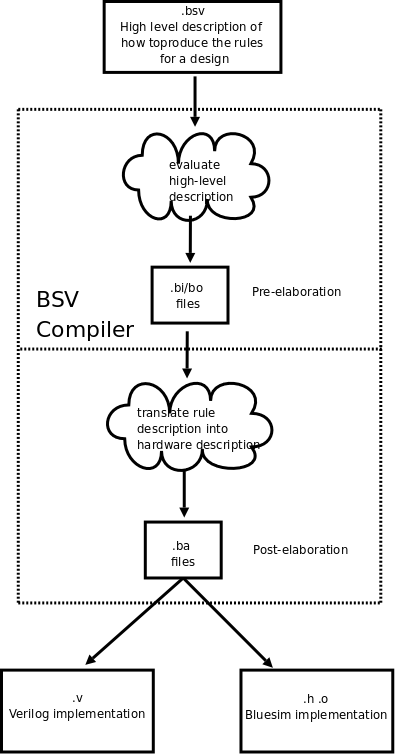
\includegraphics[angle=0, height=4.5in]{figures/compilerstages}}
  \caption{\label{compiler-stages-fig}BSV compilation stages}
\end{figure}

We  use the {\em compilation}\index{compile} stage to refer
to the two steps, type checking  and code generation, as shown inside
the dotted box in Figure \ref{compiler-stages-fig}. As the figure
shows, the  code generation specification that is output
by BSC is subject to a second run of the compiler to link
it into a simulation or synthesis environment.  We  refer to this
as the \index{link}
{\em linking} stage, even though the same compiler is used to perform
the linking.
BSC is required for
linking Bluesim generated modules.  For Verilog, the generated modules
can be handled as you would any other Verilog modules; they can be
linked with the Bluespec compiler or  you can choose to use the
generated Verilog files manually instead.

You can perform the above actions --- compile, link, and simulate ---
directly from a Unix command line.

Once you've generated the Verilog or Bluesim implementation, the
design can be analyzed using Bluetcl commands.  BSC can also dump
information during compilation and linking, via flags.

% -------------------------

\subsection{Help}

For a summary of how to run BSC and a listing of all flags, type:
\begin{centerboxverbatim}
bsc -help
\end{centerboxverbatim}
from a Unix command prompt.
Compiler flags are documented here in Section~\ref{compiler-flags}.

% -------------------------

\subsection{Compile}
\label{sec-compile}
\index{compile}
\index{type check}
\index{.bo@\te{.bo}}
\index{.ba@\te{.ba}}
\index{.v@\te{.v}}
\index{Verilog}

There are two stages in compilation, type checking and
code generation, executed by a single compile command.
The simplest compilation of a BSV design is to run only the first
stage of the compiler, generating the \te{.bo} files.
Once the type check is complete, you have enough module
information to use Bluetcl to browse the contents of packages.

The second stage (code generation) generates an elaborated module file
(\te{.ba}) and, when the target is Verilog, a (\te{.v})  file.  These
generated files have the same name as the module they implement, not
the name of the package or file they come from.

\index{attributes!synthesize}
\index{synthesize attribute@\te{synthesize} attribute}
\index{-g@\te{-g} (compiler flag)}
\index{top module}
To run the compiler through to code generation, a  module must be marked
for synthesis.  The recommended method is to use  the
\te{synthesize} attribute in the BSV code.  You can also specify a
top module with the \te{-g} compiler flag.
See Section~\ref{spec-code-gen} and the BSV Reference Guide
for information on synthesizable modules.

\index{import packages}
A  package  often imports other packages.  BSC can automatically recompile
imported packages, if necessary, if the \te{-u} option is specified on the
command line.  Section~\ref{sec-import-packages}
discusses importing packages. Section~\ref{sep-compile} contains
 a detailed explanation of  techniques and considerations
when  compiling a collection of BSV modules.

The compiler  automatically runs through to code generation if no
errors are  encountered in the type checking stage and a module is
marked for synthesis.  If errors are encountered in the type check
stage,  the compiler will halt before generating the
\te{.bo} file.  In this case, Bluetcl cannot be used to browse
the packages, as it depends on these intermediate files.
If errors are encountered in the second stage, the
\te{.bo} file will be created but the \te{.ba} file will not.
In this case, Bluetcl cannot be used to browse the modules of a
design or the scheduling of rules and methods in a design.
Library packages provided with BSC can always be browsed with
Bluetcl, since the \te{.bo} files for these packages are
always available.

\index{-sched-dot@\te{-sched-dot} (compiler flag)}
To view scheduling graphs, the compiler flag \te{-sched-dot},
described in Section~\ref{flags-sched}, must be specified for
compilation.  This flag generates the \te{.dot} files
from which graphs can be generated.

% -----

\subsubsection{Compiling a File}

A BSV source file is compiled from the command line with a command like this:
\begin{centerboxverbatim}
bsc [flags] Foo.bsv
\end{centerboxverbatim}
where one or more compiler flags may be specified after the \te{bsc} command.
Section~\ref{flags-common} describes compiling from the command line
in more detail.

If the file imports packages defined in other sources, you will need to
compile those other source files first.  BSC can be directed to
automatically compile any imported files, if necessary, before compiling
the selected file, by providing the \te{-u} flag on the command line.
The compiler compares the time stamp on the \te{.bo} file
to determine if the imported file has changed since the last
compilation.  When you compile with \te{-u}, only changed files
will be recompiled.

% -----

\subsubsection{Importing other packages}
\index{importing packages}
\label{sec-import-packages}
\index{library packages}

To compile a package that imports another package,
BSC needs the \te{.bo} file from the imported
package.  One way to provide this file is to run the compiler on
each imported file. Or direct BSC, via the \te{-u} flag, to
automatically determine which files are needed and recompile as
necessary.
If the \te{.bo} file already exists, the compiler will
only recompile if the file has changed since the last compilation, as indicated
by the imported file having a more recent date than the file being compiled.

For example, to compile  a package {\bf\tt Foo} that imports another package
{\bf\tt Baz}, BSC needs to examine the file {\bf\tt Baz.bo}. If {\bf\tt Baz} is in the file {\bf\tt
Baz.bsv},  then this file needs to be run
through the compiler to produce the necessary  {\bf\tt .bo}
file before the compiler can be invoked on {\bf\tt Foo.bsv}.
If you  use the {\bf\tt -u} flag on the command line,
the compiler will check to see if {\bf\tt Baz.bo} exists,
and if it exists, it will check the compilation date.
The compiler will recompile the {\bf\tt Baz} file if necessary.

BSC is shipped with a set of library files providing common
and useful hardware structures, such as
\te{FIFO} and \te{UInt}.  They are  described in the BSC Library
Reference Guide.   The source code for these packages is already
compiled and the  \te{.bo} files are
found in a library directory with the compiler installation (in
the same way that C header and object files are stored in standard
\emph{include} and \emph{library} directories). The compiler looks for
these files in:

\begin{centerboxverbatim}
%/Libraries/
\end{centerboxverbatim}
The BSC \te{Libraries} directory is automatically
added to the search path by BSC, unless overridden via flags.

If you are importing packages from other directories, the
directories must be added to the search path.  The flags
which modify the path are described in Section \ref{pathflags}.

% BSC also comes with a set of library files for which both the BSV
% source is provided in the \te{BSVSource} directory,
% along with compiled \te{.bo} files in the
% \te{Libraries} directory.  You can use these packages as provided, or
% edit and customize them
% to your own specifications.  To use a customized version of the these
% files, include the directory containing the \te{.bsv} source files in the search
% path. If the directory containing the  \te{.bsv} files  is in any
% position in the search path, the modified \te{.bsv} will be used, and not
% the precompiled \te{.bo} files from the \te{Libraries} directory.

% -----

\subsubsection{Specifying modules for code generation}
\label{spec-code-gen}
\index{selecting modules}
\index{code generation}
\index{-g@\te{-g} (compiler flag)}
\index{synthesize (attribute)}

A module can be selected for code generation either in the BSV code or
at compile-time.  The recommended method is to mark the module for
code generation in the BSV code, using the \te{synthesize} attribute
(see the BSV Reference Guide for more information on
attributes).  The alternative is, at compile-time, to use the
{\bf\tt -g} flag (Section~\ref{flags-common}), which instructs
the compiler to generate code for a particular module.
The {\bf\tt -g} flag can be used multiple times within a compile
command line to specify multiple modules for code generation.

Whether the generated  code will be Bluesim or Verilog depends on
which back end has been selected, by using the {\bf\tt -verilog} or
{\bf\tt -sim} command line flag.
\index{-sim@\te{-sim} (compiler flag)}
\index{-verilog@\te{-verilog} (compiler flag)}

Not all modules written in BSV are synthesizable.
To be synthesized the module must be of type \te{Module} and not of
any other module type that can be defined with \te{ModuleCollect}.
A module is synthesizable if its interface is a type whose methods and
subinterfaces are all convertible to wires.

A method is convertible to wires if it meets the following conditions:
\begin{itemize}
\item its argument types are convertible to wires which means either
\begin{itemize}
\item it is in the {\bf\tt} Bits class OR
\item it is a function whose argument and return type are convertible
to wires
\end{itemize}
\item its return type is  {\bf\tt Action} OR
\item its return type is a
{\bf\tt value} or {\bf\tt ActionValue} where  either
\begin{itemize} \item the value is convertible
to bits (i.e. in the \te{Bits} class) OR
\item the field is an exported clock or reset.
\end{itemize}
\end{itemize}
% A type is convertible to wires if it is in the {\bf\tt Bits} class or it is a
% function whose arguments and return type are convertible to wires.

A module to be synthesized is allowed to have non-interface inputs,
such as clocks and resets.  Parameters to the module are allowed
if they are convertible to bits.

Clock and Reset subinterfaces are convertible to wires.

If none of the  modules are marked for
synthesis, the compiler will not generate a hardware description (a
Verilog {\bf\tt .v} file  or a Bluesim {\bf\tt .ba} file).

% -----

\subsubsection{Understanding separate compilation}
\label{sep-compile}
\index{compilation}

BSC has two main stages; first it converts BSV modules
into a collection of states and rules, and then it converts the
rule-representation into a hardware description.

When compiling a collection of BSV modules, it is up to the user to
decide which of these modules should be compiled to hardware
separately, and which should be subsumed into the parent module.  By
default, all hierarchy is flattened into one top-level module in the
final hardware description, but the user can specify   modules which should
stay in the hierarchy and
have separate hardware descriptions.

 What happens when
a module {\bf\tt m1} instantiates another module {\bf\tt m2}?
If the submodule {\bf\tt m2} is provided as a BSV
description, that description will need to be compiled into a set of
rules and then those rules combined with the rules for {\bf\tt m1} to
be converted, by the code generation stage, into a  hardware
description.

If {\bf\tt m2} is provided as a hardware
description (that is, implemented in a Verilog file or in Bluesim header and
object files), then the hardware description for {\bf\tt m1} will
contain an instantiation of {\bf\tt m2}.  The implementation of
{\bf\tt m2} is kept in its own file.
For the Verilog back end, this produces a {\bf\tt m1.v}
file with a Verilog module {\bf\tt m1} which instantiates {\bf\tt m2}
by name and connects to its ports but doesn't contain the
implementation of {\bf\tt m2}. Both implementation files, {\bf\tt
m1.v} and {\bf\tt m2.v}, must be provided to the simulation or
synthesis tools.

\index{synthesize (attribute)}
\index{-g@\te{-g} (compiler flag)}

Even if {\bf\tt m2} is provided as a BSV description, the user can
decide to generate a separate hardware description for the module.
This is done by putting the \te{synthesize} attribute in the BSV
description   or using the
{\bf\tt -g} flag, indicating that
 the module should be synthesized
as a separate module, apart from the instantiating module.

\index{.bo@\te{.bo} (file type)}
 The
implementation in a {\bf\tt .bo} reflects whether hardware was
generated for a module.  If a hardware description was generated for a
module, then the implementation in the {\bf\tt .bo} will be merely a
pointer to the location of that description (be it {\bf\tt .v} or
{\bf\tt .o}). If hardware was not generated for the module, then an
entirely BSV representation will be stored in the {\bf\tt .bo} file.

Thus, a single {\bf\tt .bsv} file can be compiled in different ways to
produce very different {\bf\tt .bo} files.  When the
compiler is generating hardware for another BSV file that imports this
package, it will need to read in the information in the {\bf\tt .bo}
file. How it is compiled depends on the flags used. Therefore, compiling the
new file will be affected by how the imported file was compiled earlier!  It
is important, therefore, to remove these automatically generated files
before beginning a new compilation project, especially if a different
module hierarchy is desired.

For example, if a user were to generate Verilog for a module {\bf\tt mkFoo}
just for testing purposes, the {\bf\tt Foo.bo} would encapsulate into its
own description the information that a Verilog module had been generated
for module {\bf\tt mkFoo}.  If the user then wanted to generate Verilog for a
larger design, which included this module, but wanted the larger design
to be compiled into one, hierarchy-free Verilog module, then the {\bf\tt .bo} file would
have to be deleted so that a new version could be created that only
contained the state-and-rules description of the module.

% -----

\subsubsection{Interfacing to foreign modules and functions}
\index{importing foreign functions}
Foreign modules and functions can be included as part of a BSV model.
A designer can specify that the implementation of a particular BSV
module is provided as either a Verilog module or a C function.

% -----

\subsubsubsection{Importing Verilog modules}
\index{import BVI}
\index{importing Verilog}
\index{Verilog!importing}
Using the \te{import "BVI"} syntax, a designer can
specify that the implementation of a particular BSV module is an RTL
(Verilog or VHDL) module, as described in the BSV  Reference Guide.
The module is treated exactly as if it were originally
written in BSV and then converted to hardware by the compiler,  but
instead of the {\bf\tt .v} file
being generated by  the compiler, it was
supplied independently of any BSV code. It may have been written by
hand or supplied by a vendor as an IP, etc. The files for these
modules need to be linked in to the simulation.
This process is described in Section~\ref{importV-bluesim} for Bluesim simulations and
\ref{importV-verilog} for Verilog simulations.

Several primitive BSV elements, such as FIFOs and register files, are
expressed this way --- as Verilog primitives.  When simulating or
synthesizing a design generated with the Verilog back end, you will
need to include the appropriate hardware descriptions
for these primitives. Verilog descriptions for BSC's primitive
elements can be found in:

\begin{centerboxverbatim}
${BLUESPECDIR}/Verilog/
\end{centerboxverbatim}

% When compiling with the Bluesim back end, Bluesim models are needed
% instead of the Verilog files.  The Bluesim models for
% BSC's primitive elements are part of the Bluesim library
% which is linked from:

% \begin{center}
% {\small \begin{boxedverbatim}
% ${BLUESPECDIR}/Bluesim/
% \end{boxedverbatim}
% }
% \end{center}

{\bf Note:}
We attempt to be sure that the Bluesim and Verilog models simulate identically.
Simulations using 4-state (X and Z) logic, user supplied Verilog,
or other unsupported or nonstandard parts are never guaranteed to match.

% -----

\subsubsubsection{Importing C functions}
\index{import BDPI}
\index{importing C}

Using the importBDPI syntax, the user can specify that the
implementation of a BSV function is provided as a C function.
The same implementation can be used when simulating with Bluesim or
with Verilog.  In Bluesim, the imported functions are called directly.
In Verilog, the functions are accessed via the
Verilog VPI \index{Verilog Procedural Interface (VPI)}
or the SystemVerilog DPI \index{Direct Programming Interface (DPI)}.
The compilation and linking procedures for these backends are
described in Sections~ \ref{importC-bluesim} for Bluesim simulations, and
\ref{importC-verilog} for Verilog simulations.

% -------------------------

\subsection{Link}
\index{linking}
\index{link}
\label{sec-link}

The compiled  hardware description  must be linked into a simulation
environment before you can simulate the project.  The result of the linking
stage is a binary which, when executed,
simulates a module.
BSC is required for linking \index{Bluesim} Bluesim generated modules and can
be used to link Verilog\index{Verilog} modules as well.
% generated  modules can be handled as you would any other Verilog
% modules.  They can be linked via BSC
To link from the command line, use the \te{bsc}
command along with the appropriate flags, as described in Section \ref{flags-common}.

% \index{-o@\te{-o} (compiler flag)}
% The {\bf\tt -o} flag gives a name for the binary that is being created
% (here, {\bf\tt mkFoo}). If this flag is not used, the binary will have
% the default name {\bf\tt a.out}.

% -----

\subsubsection{Linking with Bluesim}
\index{Bluesim back end}
\index{Bluesim!linking .ba files}

For the Bluesim back end, linking means incorporating a set of Bluesim object
files that implement BSV modules into a Bluesim simulation
environment.  See Section \ref{bluesim-back-end} for a description of this
environment.  Bluesim is specified by using the {\bf\tt -sim} flag.
In an installation of BSC, the files for
this simulation environment are stored with the other Bluesim files
at: \verb|${BLUESPECDIR}/Bluesim/|.

Specifically, the linking stage generates a C++ object for each
elaborated module.  For each module, it generates {\em module}.\te{.h} and
{\em module}\te{.cxx} files which are compiled to a {\bf\tt .o} file.
The C++ compiler to use is determined from the {\bf\tt CXX}
environment variable (the default is {\bf\tt c++}) and any flags
specified in {\bf\tt CXXFLAGS} or {\bf\tt BSC\_CXXFLAGS} are added to
the command line.
Also generated are the files \te{model\_}{\em topmodule}\te{.h} and
\te{model\_}{\em topmodule}\te{.cxx} which are the top level that combines
the individual modules into a single model,
implementing a global schedule computed by combining the schedules from
all the individual modules in the design.
Once compiled to {\bf\tt .o} files, these objects are linked with
the Bluesim library files to produce an {\bf\tt .so} shared object
file.  This shared object file can be dynamically loaded into Bluetcl
using the {\tt sim load} command.  For convenience, a wrapper script
is generated along with the {\bf\tt .so} file which automates loading
and execution of the simulation model.

If you want to see all the \te{CAN\_FIRE} and \te{WILL\_FIRE} signals,
you must specify the \te{-keep-fires} flag (described in Section
\ref{flag-keep-fires})  when compiling and linking
with Bluesim.

The typical command to link  BSV files to generate    Bluesim
executables is:

\begin{centerboxverbatim}
bsc -sim -e -keep-fires mkFoo
\end{centerboxverbatim}

% -----

\subsubsubsection{Imported Verilog modules in Bluesim}
\label{importV-bluesim}
\index{import BVI}
\index{importing Verilog}
\index{Bluesim back end}

Using the \te{import "BVI"} syntax, a designer can specify that the
implementation of a particular BSV module is a Verilog module.  The
module is treated exactly as if it were originally written in BSV, but
was converted to hardware by the compiler.

Bluesim does not currently support importing Verilog modules
directly.  If a Bluesim back end is used to generate code for this
system,  then a
Bluesim model of the Verilog module  needs to be supplied in place
of the Verilog description.  Such a model would need to be compiled from a
BSV description and used conditionally, depending on the backend.  The
 environment
functions {\bf\tt genC} and {\bf\tt genVerilog} (as defined in the BSV
Reference Guide) can be used to determine when to compile this code.

For example, you might have a design, {\bf\tt mkDUT}, which
instantiates a submodule {\bf\tt mkSubMod}, which is a pre-existing
Verilog  file that you want to use when generating Verilog:
\begin{centerboxverbatim}
module mkDUT (...);
   ...
   SubIFC submod <- mkSubMod;
   ...
endmodule
\end{centerboxverbatim}
You would write an \te{import "BVI"} statement:
\begin{centerboxverbatim}
  import "BVI" module mkSubMod (SubIFC); ... endmodule
\end{centerboxverbatim}
But this won't work for a Bluesim simulation - Bluesim
expects a {\bf\tt .ba} file for {\bf\tt mkSubMod}.

The way to write one BSV file for both Verilog and Bluesim is to
change {\bf\tt mkSubMod} to be a wrapper, which conditionally uses a
Verilog  import or a BSV-written implementation, depending on the backend:
\begin{centerboxverbatim}
module mkSubMod (SubIFC);
   SubIFC _i <- if (genVerilog)
                   mkSubMod_verilog
                else
                   mkSubMod_bluesim;
   return _i;
endmodule

// note that the import has a different name
import "BVI" mkSubMod =
    module mkSubMod_verilog (SubIFC); ... endmodule

// an implementation of mkSubMod in BSV
module mkSubMod_bluesim (SubIfc);
   ...
endmodule
\end{centerboxverbatim}

This code will import Verilog when compiled to Verilog and
it will  use the native BSV implementation otherwise (when compiling
to Bluesim).

% -----

\subsubsubsection{Imported C functions in Bluesim}
\label{importC-bluesim}
\index{import BDPI}
\index{importing C}
\index{Bluesim back end}
\index{Bluesim!importing C functions}

Using the importBDPI syntax, the user can specify that the
implementation of a BSV functions is provided as a C function.
When compiling a BSV file
containing an import-BDPI statement, an elaboration file ({\bf\tt .ba}) is
generated for the import, containing information about the imported
function.  When linking, the user will specify the elaboration files
for all  imported functions in addition to the
elaboration files for all modules in the design.
This provides the BSC with  information  on
how to  link
to the foreign function.  In addition to this link information, the
user will have to provide access to the foreign function itself,
either as a C source file ({\bf\tt .c}), an object file ({\bf\tt .o}), or from
a library ({\bf\tt .a}).

When user provided {\bf\tt .c} files are to
be compiled and linked, the C compiler to be used is given by the
{\bf\tt CC} environment variable and the flags by the {\bf\tt CFLAGS}
and {\bf\tt BSC\_CFLAGS} variables.
The default compiler is {\bf\tt cc}.  If the extension on
the file is not {\bf\tt .c}, but {\bf\tt .cxx}, {\bf\tt .cpp} or
{\bf\tt .cc}, the C++ compiler will be used instead.
The default C++ compiler is {\bf\tt c++}, but the
compiler invocation can be controlled with the {\bf\tt CXX},
{\bf\tt CXXFLAGS} and {\bf\tt BSC\_CXXFLAGS} environment variables.

Arguments can also be passed through {\tt bsc} directly to the C
compiler, C++ compiler and linker using the {\tt\bf -Xc},
 {\tt\bf -Xc++} and {\tt\bf -Xl} options, respectively.

As an example, let's say that the user has a module {\bf\tt mkDUT}
and a testbench {\bf\tt mkTB} in the file {\bf\tt DUT.bsv}.  The testbench
uses the foreign C function {\bf\tt compute\_vector} to compute an
input/output pair for testing the design.  Let's assume that the
source code for this C function is in a file called {\bf\tt vectors.c}.
The command-line and compiler output for compiling and linking this system
would look as follows:

\begin{centerboxverbatim}
# bsc -u -sim DUT.bsv
checking package dependencies
compiling DUT.bsv
Foreign import file created: compute_vector.ba
code generation for mkDUT starts
Elaborated Bluesim module file created: mkDUT.ba
code generation for mkTB starts
Elaborated Bluesim module file created: mkTB.ba

# bsc -sim -e mkTB -o bsim mkTB.ba mkDUT.ba compute_vector.ba vectors.c
Bluesim object created: mkTB.{h,o}
Bluesim object created: mkDUT.{h,o}
Bluesim object created: model_mkTB.{h,o}
User object created: vectors.o
Simulation shared library created: bsim.so
Simulation executable created: bsim
\end{centerboxverbatim}

An elaboration file is created for the foreign name of the function,
not the BSV name that the function is imported as.  In this example,
{\bf\tt compute\_vector} is the link name, so the elaboration file is
called {\bf\tt compute\_vector.ba}.

In this example, the user provided a C source file, which bsc has compiled
into an object (here, {\bf\tt vectors.o}).  If compilation of the C
source file needs access to header files in non-default locations,
the user may specify the path to the header files with the {\bf\tt -I}
flag (see Section \ref{pathflags}).\index{-I@\te{-I} (compiler flag)}

If the user has a pre-compiled object file or library, that file can
be specified on the link command-line in place of the source file.
In that situation, BSC does not need to compile
an object file, as follows:

\begin{centerboxverbatim}
# bsc -sim -e mkTB -o bsim mkTB.ba mkDUT.ba compute_vector.ba vectors.o
Bluesim object created: mkTB.{h,o}
Bluesim object created: mkDUT.{h,o}
Bluesim object created: model_mkTB.{h,o}
Simulation shared library created: bsim.so
Simulation executable created: bsim
\end{centerboxverbatim}

In both situations, the object file is finally linked with the Bluesim
design to create a simulation binary.  If the foreign function uses any
system libraries, or is itself a system function, then the linking stage
will need to include those libraries.
From the command line, the user can specify libraries to
include with the {\bf\tt -l} flag and can specify non-default paths to
the libraries with the {\bf\tt -L} flag (see Section \ref{pathflags}).\index{-L@\te{-L} (compiler flag)}
\index{-l@\te{-l} (compiler flag)}

% -----

\subsubsection{Creating a SystemC Model Instead of a Bluesim Executable}
\index{SystemC back end}
\index{SystemC!linking .ba files}
\index{-systemc@\te{-systemc} (compiler flag)}
\label{flag-systemc}

Instead of linking {\bf\tt .ba} files into a Bluesim executable, the linking
stage can be instructed to generate a SystemC model by replacing the
{\bf\tt -sim} flag with the {\bf\tt -systemc} flag.  All other aspects
of the linking stage, including the use of environment variables, the
object files created, and linking in external libraries, are identical to
the normal Bluesim tool flow.

When using the {\bf\tt -systemc} flag, the object files created to
describe the design in C++ are not linked into a Bluesim executable.
Instead, some additional files are created to provide a SystemC
interface to the compiled model.  These additional SystemC files use
the name of the top-level module extended with a \te{\_systemc} suffix.

\begin{centerboxverbatim}
# bsc -sim GCD.bsv
Elaborated Bluesim module file created: mkGCD.ba

# bsc -systemc -e mkGCD mkGCD.ba
Bluesim object created: mkGCD.{h,o}
Bluesim object created: model_mkGCD.{h,o}
SystemC object created: mkGCD_systemc.{h,o}
\end{centerboxverbatim}

Remember to define the \te{SYSTEMC} environment variable to point at
your SystemC installation (See Section \ref{app-env}).

There are a few additional restrictions on models with which
{\bf\tt -systemc} can be used.  The top-level interface of the model
must not contain any combinational paths through the interface.  For
the same reason, ActionValue methods and value methods with arguments
are not allowed in the top-level interface.

Additionally, value methods in the top-level interface must be free
of scheduling constraints that require them to execute after rules
in the design.  This means that directly registered interfaces are the
most suitable boundaries for SystemC model generation.

The SystemC model produced is a clocked, signal-level model.
Single-bit ports use the C++ type {\tt bool}, and wider ports use the
SystemC type {\tt sc\_bv<N>}.  Subinterfaces (if any) are flattened
into the top-level interface.  The names of ports obey the same naming
conventions (and the same port-naming attributes) as the Verilog backend
(See Section~\ref{sec-vl-name-mapping}).

The SystemC model interface is defined in the produced {\bf\tt .h}
file, and the implementation of the model is split among the various
{\bf\tt .o} files produced.  The SystemC model can be instantiated
within a larger SystemC design and linked with other SystemC objects
to produce a final system executable, or it can be used to cosimulate
inside of a suitable Verilog or VHDL simulator.

\begin{center}
\begin{tabular}{|l|l|}
\hline
\multicolumn{2}{|c|}{Division of Functionality Among Files} \\
\hline
\multicolumn{1}{|c|}{File} & \multicolumn{1}{|c|}{Purpose} \\
\hline
{\em module}\te{.\{cxx,h,o\}} & Implementation of modules \\
\te{model\_}{\em topmodule}\te{.\{cxx,h,o\}} & Implementation of the full design and schedule \\
{\em topmodule}\te{\_systemc.\{cxx,h,o\}} & Top-level SystemC interface \\
\hline
\end{tabular}
\end{center}

The {\em module}\te{.\{cxx,h,o\}} files contain the implementations of the modules,
each as its own C++ class.  The classes have methods corresponding to
the rules and methods in the BSV source for the module and member
variables for many logic values used in the implementation of the
module.

The \te{model\_}{\em topmodule}\te{.\{cxx,h,o\}} files combine the
individual modules into a single model, defined as a C++ class.
The class contains the scheduling logic which
sequences rules and method calls and enforces the scheduling
constraints during rule execution.  The scheduling functions are
called only through the simulation kernel, never directly from user
code.

The {\em topmodule}\te{\_systemc.\{cxx,h,o\}} files contain the
top-level SystemC module
for the system.  This module is an SC\_MODULE with ports for the
module clocks and resets as well as for the signals associated with
each method in the top-level interface.  Its constructor instantiates
the implementation modules and initializes the simulation kernel.
Its destructor shuts down the simulation kernel and releases the
implementation module instances.  The SystemC module contains
SC\_METHODs which are sensitive to the module's clocks and transfer
data between the SystemC environment and the implementation classes,
translating between SystemC data types and BSV data types.

When linking the produced SystemC objects into a larger system, all of
the {\bf\tt .o} files produced must be linked in, as well the standard
SystemC libraries and Bluesim kernel and primitive libraries.

\begin{centerboxverbatim}
# c++ -I/usr/local/systemc-2.1/include -L/usr/local/systemc-2.1/lib-linux \
      -I$BLUESPECDIR/Bluesim -L$BLUESPECDIR/Bluesim \
      -o gcd.exe mkGCD.o mkGCD_systemc.o model_mkGCD.o top.cxx TbGCD.cxx \
      -lsystemc -lbskernel -lbsprim -lpthread
\end{centerboxverbatim}

% -----

\subsubsection{Linking with Verilog}
\index{Verilog back end}
\index{Verilog!linking}
\index{Verilog!simulator}

For the Verilog back end, linking means invoking a Verilog compiler to create a
simulator binary file or a script to execute and run the
simulation. Section~\ref{sec-vl-back-end} describes the Verilog
output  in more
detail.  The Verilog simulator is specified by  using the {\bf\tt
-vsim} flag.

\index{Verilog simulator!cvc}
\index{Verilog simulator!cver}
\index{Verilog simulator!isim}
\index{Verilog simulator!iverilog}
\index{Verilog simulator!modelsim}
\index{Verilog simulator!ncverilog}
\index{Verilog simulator!questa}
\index{Verilog simulator!vcs}
\index{Verilog simulator!vcsi}
\index{Verilog simulator!verilator}
\index{Verilog simulator!veriwell}
\index{Verilog simulator!xsim}

\index{cvc (Verilog simulator)}
\index{cver (Verilog simulator)}
\index{isim (Verilog simulator)}
\index{iverilog (Verilog simulator)}
\index{modelsim (Verilog simulator)}
\index{ncverilog (Verilog simulator)}
\index{questa (Verilog simulator)}
\index{vcs (Verilog simulator)}
\index{vcsi (Verilog simulator)}
\index{verilator (Verilog simulator)}
\index{veriwell (Verilog simulator)}
\index{xsim (Verilog simulator)}

\index{-vsim@\te{-vsim} (compiler flag)}

\label{sec:using-verilog}
The \textbf{\texttt{-vsim}} flag
(along with the equivalent
\textbf{\texttt{BSC\_VERILOG\_SIM}} environment variable) governs which Verilog
simulator is employed; at present, natively supported choices for
\textbf{\texttt{-vsim}} are
\texttt{cvc},
\texttt{cver},
\texttt{isim}.
\texttt{iverilog},
\texttt{modelsim},
\texttt{ncverilog},
\texttt{questa},
\texttt{vcs},
\texttt{vcsi},
\texttt{verilator},
\texttt{veriwell},
and \texttt{xsim}.
If the simulator is not specified \texttt{bsc} will attempt to detect one
of the above simulators and use it.

When the argument to \textbf{\texttt{-vsim}} contains the slash character
(\texttt{/}), then the argument is interpreted as the name of a script to run
to create the simulator binary.  Indeed, the predefined simulator names listed
above refer to scripts in the BSC distribution; thus,
\texttt{-vsim vcs} is equivalent to \texttt{-vsim
\$BLUESPECDIR/lib/exec/bsc\_build\_vsim\_vcs}.  The simulator scripts distributed
with BSC are good starting points should the need to use an unsupported
simulator arise.

In some cases, you may want to append additional flags to the
Verilog simulator command that is used to generate the simulator
executable. The \textbf{\texttt{BSC\_VSIM\_FLAGS}} environment
variable is used for this purpose.
% Thus, for instance, setting its
% value to \texttt{-y verilog\_libs} will add the directory
% \texttt{verilog\_libs} to the simulator search path (for simulators
% such as \texttt{iverilog} and \texttt{vcs}).

To add  directories to the search path when linking Verilog designs,
use the \te{-vsearch}\index{-vsearch@\te{-vsearch} (compiler flag)} flag,
described in Section~\ref{pathflags}.  For example, adding the flag \te{-vsearch
+:verilog\_libs} to the BSC command will add the directory
\te{verilog\_libs} to the simulator search path (for simulators such
as \te{iverilog} and \te{vcs/vcsi}).  This is equivalent to adding \te{-y
<directory>} to the Verilog compilation command.

The generated Verilog can be put into a larger Verilog design, or run
through any existing Verilog tools.  BSC also provides a
convenient way to link the generated Verilog into a simulation using  a
top-level module (\te{main.v}) to provide a clock for the design.  The
BSC-provided \te{main.v} module instantiates the top module
and toggles the clock every five simulation time units.
From the command line the following
command  generates a simulation binary \te{mkFoo.exe}:

\begin{centerboxverbatim}
bsc -verilog -e mkFoo -o mkFoo.exe
\end{centerboxverbatim}

With this command the top level Verilog module \te{main} is taken from
\te{main.v}.  \te{main.v} provides a clock and a reset, and
instantiates \te{mkFoo}, which should provide an \te{Empty}
interface.  An executable file, \te{mkFoo.exe} is created.

\index{+bscvcd@\te{+bscvcd} (Verilog simulation)}
\index{+bsccycle@\te{+bsccycle} (Verilog simulation)}
\index{VCD!Verilog}
\index{FSDB!Verilog}
\index{value change dump!Verilog}
\label{plusarg}

The default \te{main.v} allows two plusarg arguments to be used during
simulation:
\te{+bscvcd} and \te{+bsccycle}.  The argument \te{+bscvcd}  generates
a value change dump file (VCD) or a FSDB file;   \te{+bsccycle} prints a
message each clock cycle.  These are specified from the command line:
\begin{centerboxverbatim}
./mkFoo.exe +bscvcd +bsccycle
\end{centerboxverbatim}

% -----

\subsubsubsection{BSC pre-processor macros}

\label{sec-preprocessor-macro}

When linking with BSC Verilog files (including \te{main.v}),  the
following pre-processor macros can be used to  impact the
behavior of the Verilog simulation.
The \te{-D} flag, which defines macro values for the \te{`defines}
statements  must be specified, as described in Section
\ref{flags-misc}.  These macros are specified when you link the
simulation executable, not during runtime.

\begin{tabular}{|p{1.4 in}|p{2.2in}|p{2 in}|}
\hline
\multicolumn{3}{|c|}{BSC Verilog Macros}\\
\hline
Name&Description&Example\\
\hline\hline
\te{BSV\_ASSIGNMENT\_DELAY}& Delays assignment at the start of
simulation.&\verb$-D BSV_ASSIGNMENT_DELAY = #0$\\
\hline
\te{BSV\_TIMESCALE}& Sets the timescale of the simulation.
&\verb$-D BSV_TIMESCALE = 1ns/1ps$\\
\hline
\te{BSV\_NO\_INITIAL\_BLOCKS}& Sets initial values to \te{X} at
the start of simulation.&\verb$-D BSV_NO_INITIAL_BLOCKS$\\
\hline
\te{BSV\_FSDB}&Generates a FSDB file during simulation.&\verb$-D BSV_FSDB$\\
\hline
\te{BSV\_POSITIVE\_RESET}&Changes the sense of reset to asserted hi
from asserted low&\verb$-D BSV_POSITIVE_RESET$\\
\hline
\te{BSV\_ASYNC\_RESET}& Use \te{ASYNC} reset for FIFO packages and
packages using  \te{Counter.v} &\verb$-D BSV_ASYNC_RESET$ \\
\hline
\te{BSV\_RESET\_FIFO\_HEAD} & Allow reset on head element of FIFO&\verb$-D BSV_RESET_FIFO _HEAD$\\
\hline
\te{BSV\_RESET\_FIFO\_ARRAY}& Allow reset on array elements of FIFO&\verb$-D BSV_RESET_FIFO_ARRAY$\\
\hline
\end{tabular}

% When using a positive reset, the following flags are recommended for
% both the compile and link stages:
% \begin{centerboxverbatim}
% -reset-prefix "RESET_P" -D BSV_POSITIVE_RESET
% \end{centerboxverbatim}

% -----

\subsubsubsection{Imported Verilog functions in Verilog}
\label{importV-verilog}
\index{Verilog back end}
\index{importing Verilog}
\index{.xcf@\te{.xcf} (synthesis script)}
\index{Xilinx synthesis script}

When Verilog code is generated for a system that uses a
Verilog-defined module, the generated code  contains an
instantiation of this Verilog module with the assumption that the
{\bf\tt .v} file containing its definition is available
somewhere. This file is needed if the full system is to be
simulated or synthesized (the linking stage).  \index{VHDL} Note that
VHDL modules
can be used instead of Verilog modules if your simulator supports
mixed language simulation.

 When simulating or
synthesizing a design generated with the Verilog back end, you
need to include the Verilog descriptions for these primitives.  The
Verilog descriptions for BSC's primitive elements (FIFOs,
registers, etc.)
can be found in:

\begin{centerboxverbatim}
${BLUESPECDIR}/Verilog/
\end{centerboxverbatim}

This directory also contains the file  \te{Bluespec.xcf},  a Xilinx XCF
constraint file to be used when synthesizing with Xilinx. 

% -----

\subsubsubsection{Imported C functions in Verilog}
\label{importC-verilog}
\index{Verilog back end}
\index{importing C}
\index{Verilog Procedural Interface (VPI)}
\index{Direct Programming Interface (DPI)}

In a BSV design compiled to Verilog, foreign functions are simulated
using either the Verilog Procedural Interface (VPI) or the SystemVerilog
Direct Programming Interface (DPI).  The default is to use VPI, unless
the \te{-use-dpi} flag is provided (see Section \ref{sec-verilogflags}).

For VPI, the generated Verilog
calls a user-defined system task anywhere the imported function is
needed.  The system task is implemented as a C function which is a
wrapper around the user's imported C function, to handle the VPI
protocols.

For DPI, the generated Verilog calls a function anywhere the imported
function is needed.  That function is declared as an import-DPI function
at the top of the file.  In most cases, the declaration imports the user's
C function directly, without a wrapper, because SystemVerilog's DPI types
closely match BSV's BDPI types.  As a result, using DPI is likely more
efficient than using VPI, though some simulators may only support one.
For polymorphic BDPI functions, the DPI and BDPI types differ and so a
wrapper is needed.  BSC does not yet support generating the DPI wrapper.

The usual Verilog flow is that BSV modules are generated to Verilog
files, which are linked together into a simulation binary.  The user
has the option of doing the linking manually or by calling BSC.
Imported functions can be linked in either case.

\index{import BDPI}
As with the Bluesim flow, when compiling a BSV file containing an
import-BDPI statement, an elaboration file is generated for the import,
containing information about the imported function.  However, with Verilog
generation, a wrapper function may also be generated.  For example,
using the scenario from the previous section but compiling to Verilog,
and using VPI, the user would see the following:

\begin{centerboxverbatim}
# bsc -u -verilog DUT.bsv
compiling DUT.bsv
Foreign import file created: compute_vector.ba
VPI wrapper files created: vpi_wrapper_compute_vector.{c,h}
code generation for mkDUT starts
Verilog file created: mkDUT.v
code generation for mkTB starts
Verlog file created: mkTB.v
\end{centerboxverbatim}

The compilation of the import-BDPI statement has not only generated
an elaboration file for the input but has also generated the file
{\bf\tt vpi\_wrapper\_compute\_vector.c} (and associated header file).
This file contains
both the wrapper function {\bf\tt compute\_vector\_calltf()} as
well as the registering function for the wrapper,
{\bf\tt compute\_vector\_vpi\_register()}.
The registering function is what tells the Verilog simulator about the
user-defined system task.  Included in the comment at the top of the
file is information needed for linking manually.

When linking manually, this C file typically needs to be compiled to
an object file ({\bf\tt .o} or {\bf\tt .so}) and provided on the
command line to the Verilog linker, along with the object files for
the user's function (in this example, {\bf\tt vectors.c}).  The
Verilog linker also needs to be told about the registering function.
For some Verilog simulators, the registering function is named on the
command-line.  For other simulators, a C object file must be created
containing the array {\bf\tt vpi\_startup\_array} with pointers to all
of the registering functions (to be executed on start-up of the
simulation).  An example of this start-up array is given in the comment
at the top of the generated wrapper C files.  Some simulators require
a table for imported system functions (as opposed to system tasks).
The table is provided in a file with {\bf\tt .tab} or {\bf\tt .sft}
extension.  The text to be put in these files is also given in the
comment at the top of the wrapper file.  The text also appears later
in the file with the tag ``{\bf\tt tab:}'' or ``{\bf\tt sft:}''
prepended.  A search for the appropriate tag (with a tool like {\bf\tt grep})
will extract the necessary lines to create the table file.

Linking via BSC does all of this automatically:

\begin{centerboxverbatim}
# bsc -verilog -e mkTB -o vsim mkTB.v mkDUT.v compute_vector.ba vectors.c
VPI registration array file created: vpi_startup_array.c
User object created: vectors.o
VPI object created: vpi_wrapper_compute_vector.o
VPI object created: vpi_startup_array.o
Verilog binary file created: vsim
\end{centerboxverbatim}

To perform linking via BSC, the user provides on the command-line not
only the Verilog files for the design but also the foreign import files
({\bf\tt .ba}) for each imported function and the C source or object files
implementing the foreign functions.  As shown in the above example,
the linking process will create the file {\bf\tt vpi\_startup\_array.c},
containing the registration array, and will compile it to an object file.
The linking process will then pass all of the VPI files along to the
Verilog simulation build script (see Section~\ref{sec:using-verilog})
which will create any necessary table files and invoke the Verilog
simulator with the proper command-line syntax for using VPI.

Using DPI is a simpler process.  No separate registration files are
needed because the imported function is declared by a
SystemVerilog import-DPI statement in the generated Verilog itself.
And for most import-BDPI functions, no wrappers are generated either.
This makes manual linking particularly easier, although linking via
BSC is also possible using DPI.  The Verilog simulation build script
will consult the BSC flags to determine whether imported functions are
to be provided to the simulator as DPI or VPI.
It is therefore necessary to use the same flags for choosing DPI/VPI
during linking as were used during compilation.

If the foreign function uses any system libraries, or is itself a
system function, then the Verilog linking will need to include those
libraries.  As with the Bluesim flow, the user can specify to BSC
the libraries to include with the {\bf\tt -l} flag and can specify
non-default paths to the libraries with the {\bf\tt -L} flag
(see Section~\ref{pathflags}).\index{-L@\te{-L} (compiler flag)}
\index{-l@\te{-l} (compiler flag)}

% -------------------------

\subsection{Simulate}
\label{simulate}
\index{FSDB}
\index{VCD}

The result of linking is a simulation executable.

You can generate a VCD file from either Bluesim or any of the
 supported Verilog simulators.  When simulating with Bluesim, use
 the \te{-V} flag.   For Verilog simulators using
the BSC-provided \te{main.v} file, specify the \te{+bscvcd} flag during
simulation.

To dump a FSDB file directly from a supported Verilog simulator using
the BSC-provided \te{main.v} file, you  need to specify the
\te{+bscvcd} flag during simulation and the  \te{-D BSV\_FSDB} flag
during linking.
Note that not all simulators can generate an FSDB file.
Additional command line arguments are required, dependent on the simulator.
Bluesim does not generate FSDB files at this time.

% ------------------------------------------------------------

\section{BSC flags}

\label{compiler-flags}
\index{bsc flags}

You can obtain an up-to-date
listing of the available flags along with brief explanations by going
to a Unix command line and entering:

\begin{centerboxverbatim}
bsc  -help
\end{centerboxverbatim}

\index{-help@\te{-help} (compiler flag)}
\index{-no@\te{-no} (compiler flag)}
Most flags may be preceded by a {\bf\tt -no} to reverse their
effect. Flags that appear later on the command line override earlier
ones.

The following flags make the compiler print more or less progress-report
messages as it does its work:

\index{-quiet@\te{-quiet} (compiler flag)}
\index{-q@\te{-q} (compiler flag)}
\index{-verbose@\te{-verbose} (compiler flag)}
\index{-v@\te{-v} (compiler flag)}
\begin{centerboxverbatim}
-quiet                be less talkative
-q                    same as -quiet
-verbose              be more talkative
-v                    same as -verbose
\end{centerboxverbatim}

The compiler has four levels of verbosity: quiet, normal, verbose,
and extra verbose.  The default is normal verbosity and the above
flags can be used to move up and down one step.

% -------------------------

\subsection{Common compile and linking flags}
\index{compile flags}
\index{linking flags}
\label{flags-common}

The following flags are the common flags used by the compiler.

\index{-g@\te{-g} (compiler flag)}
\index{-u@\te{-u} (compiler flag)}
\index{-verilog@\te{-verilog} (compiler flag)}
\index{-sim@\te{-sim} (compiler flag)}
\index{-vsim@\te{-vsim} (compiler flag)}
\index{-e@\te{-e} (compiler flag)}
\index{-o@\te{-o} (compiler flag)}
\index{-elab@\te{-elab} (compiler flag)}
\begin{centerboxverbatim}
-g module             generate code for `module' (requires -sim or -verilog)
-u                    check and recompile packages that are not up to date
-sim                  compile BSV generating Bluesim object
-verilog              compile BSV generating Verilog file
-vsim simulator       specify which Verilog simulator to use
-e module             top-level module for simulation
-o name               name of generated executable
-elab                 generate a .ba file after elaboration and scheduling
\end{centerboxverbatim}


A BSV source file is compiled with a command like this:
\begin{center}
\begin{smbox}
{\tt \hspace*{2em} bsc}\hspace*{2em}[\emph{flags}]\hspace*{2em}{\tt Foo.bsv}
\end{smbox}
\end{center}
where \te{Foo.bsv} is the top file in the design.

If no flags are provided, the compile stops after  the type
checking phase.  To compile through code generation, you must provide a
flag indicating whether the target is Bluesim (\te{-sim}) or
Verilog  (\te{-verilog}).

For example, to compile to code generation for Bluesim:
\begin{centerboxverbatim}
bsc -sim Foo.bsv
\end{centerboxverbatim}
or for Verilog:
\begin{centerboxverbatim}
bsc -verilog Foo.bsv
\end{centerboxverbatim}

As discussed in Section \ref{spec-code-gen}, when compiling to
code generation  a module must be specified, using either  the \te{synthesize}
attribute in the BSV code, or  the {\bf\tt -g} flag at compile
time.  From the command line,
multiple modules can be specified for code generation at the same time.

For example:
\begin{centerboxverbatim}
bsc -sim -g mkFoo -g mkBaz Foo.bsv
\end{centerboxverbatim}

Linking requires a second call to the compiler, as described in
Section \ref{sec-link}.  When linking you must specify the
top-level module with the {\bf\tt -e} flag.  The name following the
flag must be the name of  a BSV module and only one module can be
specified.   You must also specify the back end with either the
{\bf\tt -sim}   or {\bf\tt -verilog} flag.

For example, to link for Bluesim:
\begin{centerboxverbatim}
bsc -sim -e mkFoo
\end{centerboxverbatim}
or for Verilog:
\begin{centerboxverbatim}
bsc -verilog -e mkFoo
\end{centerboxverbatim}


The \te{-vsim} flag
(along with the equivalent
\textbf{\texttt{BSC\_VERILOG\_SIM}} environment variable) governs which Verilog
simulator is employed.  The natively supported  choices for
\te{-vsim} are
\te{cvc},
\te{cver},
\te{isim}.
\te{iverilog},
\te{modelsim},
\te{ncverilog},
\te{questa},
\te{vcs},
\te{vcsi},
\te{verilator},
\te{veriwell},
and \te{xsim}.
If a simulator is not specified \te{bsc} will attempt to detect one
of the above simulators and use it.


When using Bluetcl (or applications built on Bluetcl) to analyze a compiled
design, a \te{.ba} file is required (for each module in the design).
To generate this file when compiling add the \te{-elab} flag to the compile command. 


% -------------------------

\subsection{Controlling default flag values}
\index{BSC\_OPTIONS@\te{BSC\_OPTIONS}}

The environment variable \te{BSC\_OPTIONS} enables the user to set
default flag values to be used each time the compiler is called.  If
set, the value of \te{BSC\_OPTIONS} is automatically  prepended to the
compiler option values  typed on the bsc command line.  This avoids
the need to set specified flag values each time the compiler is called.

% BSC recognizes  the environment variable
% \te{BSC\_OPTIONS}.  If set, the value of \te{BSC\_OPTIONS} is
% automatically  prepended to the
% values on the bsc command line. This allows the user to set default
% flag  values and avoid the need to set them each time the compiler is called.

For instance, in order to control the default value of the \te{-p} (path)
option, the \te{BSC\_OPTIONS} environment variable could be set as follows:

\begin{centerboxverbatim}
# BSC Environment for csh/tcsh
setenv BSC_OPTIONS "-p .:./MyLib:+"

# BSC Environment for bash/ksh
export BSC_OPTIONS="-p .:./MyLib:+"
\end{centerboxverbatim}


Once set, BSC would now search for packages in the
\te{./MyLib} directory before looking in the default library
areas. Note that since the compiler  recognizes multiple uses of
the same flag on the command line, the user can use the \te{-p}
flag along with  the \te{BSC\_OPTIONS} environment variable to control
the search path. For example, if in addition to the \te{BSC\_OPTIONS}
set above the user enters the following bsc
command, :

\begin{centerboxverbatim}
    bsc -verilog -p ./MyLib2:+ Foo.bsv
\end{centerboxverbatim}

the compiler would now use the path

\begin{centerboxverbatim}
    ./MyLib2:.:./MyLib:+
\end{centerboxverbatim}

which is a prepending of the \te{-p} command line value to the value set by the
\te{BSC\_OPTIONS} environment variable.


% -------------------------

\subsection{Verilog back-end}
\label{sec-verilogflags}
\index{Verilog flags}
\index{Verilog back end}
The following additional flags are available when using the Verilog
back end.
\index{-remove-unused-modules@\te{-remove-unused-modules} (compiler
flag)}
\index{-v95@\te{-v95} (compiler flag)}
\index{-remove-dollar@\te{-remove-dollar} (compiler flag)}
\index{-unspecified-to@\te{-unspecified-to} (compiler flag)}
\index{-Xv@\te{-Xv} (compiler flag)}
\index{-verilog-filter@\te{-verilog-filter} (compiler flag)}
\index{-use-dpi@\te{-use-dpi}}
\begin{centerboxverbatim}
-remove-unused-modules  remove unconnected modules from the Verilog
-v95                    generate strict Verilog 95 code
-unspecified-to val     remaining unspecified values are set to:
                         'X', '0', '1', 'Z', or 'A'
-remove-dollar          remove dollar signs from Verilog identifiers
-Xv arg                 pass argument to the Verilog link process
-verilog-filter cmd     invoke a command to post-process the generated Verilog
-use-dpi                use DPI instead of VPI in generated Verilog
\end{centerboxverbatim}

The {\bf\tt -remove-unused-modules} flag will remove from the generated
Verilog any modules which are not connected to an
output.  This has has the effect of removing redundant or unused
modules, which would also be done by synthesis tools.   This option
should be used on modules undergoing synthesis, and not be used for
testbench modules.

The {\bf\tt -v95} flag restricts the Verilog output to pure Verilog-95.
By default, the Verilog output uses features which are not in the
Verilog-95 standard.  These features include passing module
parameters by name and use of the {\tt \$signed} system task for formatting
{\tt \$display} output.  When the {\tt -v95} flag is turned on, uses
of these features are removed, but comments are left in the Verilog
indicating the parameter names or system tasks which were removed.

The {\bf\tt -unspecified-to val} flag defines the value
which any remaining unspecified values should be tied to.  The valid
set of values are: {\tt X}, {\tt 0}, {\tt 1}, {\tt Z}, or {\tt A},
where the first four correspond to the Verilog value, and {\tt A}
corresponds to a vector of alternating ones and zeros.
The default value is {\tt A}.  The choice of value is used by both
the Verilog and Bluesim back ends.  However, since Bluesim is a two-value
simulator, it does not support the values {\tt X} and {\tt Z}.
For final synthesis runs, the use of {\tt X} (or {\tt 0})
is strongly suggested to give the best synthesis results.

The {\bf\tt -remove-dollar} flag causes identifiers in Verilog output
to substitute underscores instead of dollar signs to separate instance
names from port names.  If this substitution causes a name collision,
the underscore is suffixed with a number until a non-colliding name is
found.

The {\bf\tt -Xv} flag passes the specified string argument to the Verilog link
process.   Only one argument can be passed with each {\bf\tt -Xv}
flag. If you want to pass multiple arguments, then the flag must be
specified multiple times, once for each argument.

The {\bf\tt -verilog-filter} flag invokes a command to process the
 Verilog file generated by the compiler.  The command can be a Unix
 command or script;
it must take a single argument, the name of the Verilog file.    The
 flag can be used multiple times; the filters are applied in the order
 they are given on the command line.

The {\bf\tt -use-dpi} flag controls whether imported C functions in
source designs are implemented in Verilog using
the Verilog Procedural Interface (VPI)
\index{Verilog Procedural Interface (VPI)}
or the SystemVerilog Direct Programming Interface (DPI)
\index{Direct Programming Interface (DPI)}.
The flag must be consistently used during both the compilation and
linking steps.
During compilation, the flag controls how imported C calls appear
in the generated Verilog;
during linking, the flag controls how the C functions are provided
to the simulator.
By default, this flag is \emph{off} and VPI is used.


% -------------------------

\subsection{Bluesim back-end}
\label{sec-bluesimflags}
\index{Bluesim flags}
\index{Bluesim back end}
The following  flags are available when using the Bluesim
back end.
\index{-parallel-sim-link@\te{-parallel-sim-link} (compiler flag)}
\index{-systemc@\te{-systemc} (compiler flag)}

\begin{centerboxverbatim}
-parallel-sim-link jobs     specify the # of simultaneous jobs when linking Bluesim
-systemc                    generate a SystemC model
\end{centerboxverbatim}

During the Bluesim linking process, the compiler generates C++ source
files (\te{.cxx} and \te{.h} files) and then runs the C++ compiler on
each one.  By default, these compilations are performed serially.  In
some cases, the C++ compiler may take time to compile a file.  In that
case, it would be helpful to compile other files in parallel to
reduce the total compilation time.
The \te{-parallel-sim-link} flag directs the process to proceed in
parallel,  up to {\em jobs} number of simultaneous compilations.

The default value of {\em jobs} is 1, in which case the compilation
occurs in serial.  Only values greater than 1 will allow parallel compilations.

When compilation occurs in parallel, it is controlled by a Makefile,
described in Appendix \ref{app-make}.  When the verbose (\te{-v}) flag
is used to compile, you will now see the command for the \te{make}
excecution.  The commands for compiling each object will still be
shown as well.  Since the compilations are
happening in parallel, the messages will be interspersed with each
other and will not show up in serial order (Section \ref{sec-progress-messages}). 

The {\bf\tt -systemc} flag instructs the linking stage to generate a
SystemC model instead of a Bluesim executable (Section \ref{flag-systemc}).  When using this flag,
the object files created to describe the design in C++ are not linked
into a Bluesim exectuable.  Instead, some additional files are created
to provide a SystemC interface to the compiled model.  These
additional SystemC files use the name of the top-level module extended
with a \te{\_systemc} suffix.  

% -------------------------

\subsection{Resource scheduling (all back ends)}
\label{resource-sched}
\index{Verilog back end}
\index{Bluesim back end}
\index{resource scheduling}
The following flags are available to direct resource scheduling:
\index{-resource-off@\te{-resource-off} (compiler flag)}
\index{-resource-simple@\te{-resource-simple} (compiler flag)}
\begin{centerboxverbatim}
-resource-off           fail on insufficient resources
-resource-simple        reschedule on insufficient resources
\end{centerboxverbatim}

Resource scheduling for a particular interface method involves finding
all rules that call that method. A single method name can refer to
multiple ports in the hardware --- for example, a double-ported RAM
can have two \emph{read} ports, but a design in BSV can use the name
{\bf\tt read} and it will rely on the compiler to determine which port
is being used. If the number of rules that use {\bf\tt read} is two or
less, then there is no problem; each rule is connected to its own port
and there is never any contention. If the number of rules vying for a
method is more than the number of copies of that method, then a
problem exists.

If {\bf\tt -resource-off} is specified, the compiler will give up and
tell the user that resource scheduling is not possible. This is the
default behavior. The straightforward way to proceed is by adding logic that
explicitly arbitrates between the competing rules (choosing the more
important one to fire depending on the situation).

The alternative way to resolve a resource conflict is to block competing
rules until the number of rules vying for a method is less than the
number of available ports for that method.  This behavior can be turned
\emph{on} with the {\bf\tt -resource-simple} flag. The compiler selects
rules to block from the competing rules arbitrarily (and may change its
selection when different compilation flags or compiler versions are used),
so this flag is not recommended for a completed design, but automatic resource
arbitration can be useful when experimenting.


% -------------------------

\subsection{Setting the path}
\index{path flags}

\label{pathflags}
\index{-i@\te{-i} (compiler flag)}
\index{-p@\te{-p} (compiler flag)}
\index{-bdir@\te{-bdir} (compiler flag)}
\index{-simdir@\te{-simdir} (compiler flag)}
\index{-vdir@\te{-vdir} (compiler flag)}
\index{-vsearch@\te{-vsearch} (compiler flag)}
\index{-info-dir@\te{-info-dir} (compiler flag)}
\index{-I@\te{-I} (compiler flag)}
\index{-l@\te{-l} (compiler flag)}
\index{-fdir@\te{-fdir} (compiler flag)}

\begin{centerboxverbatim}
-i dir                  override $BLUESPECDIR
-p path                 directory path (`:' sep.) for source and intermediate
                        files
-bdir dir               output directory for .bo and .ba files
-simdir dir             output directory for Bluesim intermediate files
-vdir dir               output directory for .v files
-vsearch path           search path (`:' sep.) for Verilog files
-info-dir dir           output directory for informational files
-I path                 include path for compiling foreign C/C++ source
-L path                 library path for linking foreign C/C++ objects
-l library              library to use when linking foreign C/C++ objects
-fdir dir               working directory for relative file paths during elaboration 
\end{centerboxverbatim}

There are default locations where the compiler looks for source and
and intermediate files.
The flags {\bf\tt -i} and {\bf\tt -p} are available to override the
default locations or to specify additional directories to search in.
See Section \ref{sec-import-packages} for more information.  The {\bf\tt -i} flag
overrides the environment variable {\bf\tt BLUESPECDIR}, which is used
in the default value for the directory path of the  {\bf\tt -p} flag.
The {\bf\tt -p} flag
takes a path argument, which is a colon-delimited list of
directories. This path is used to find Bluespec source and intermediate
files imported by the
package being compiled (including the standard prelude, and files included
by the BSV preprocessor). The path can
contain the character {\bf\tt \%}, representing the {\bf\tt BLUESPECDIR}
directory, as well as {\bf\tt +}, representing the current path. The
default path is: \nopagebreak

\begin{centerboxverbatim}
.:%/Libraries
\end{centerboxverbatim}


The {\bf\tt -bdir}, {\bf\tt -simdir}, {\bf\tt -vdir},
and {\bf\tt -info-dir} \label{flag-info-dir} flags specify
where output files should be placed. The default is the directory in
which the input file(s) reside.

The {\bf\tt -vsearch} flag  specifies the search path used
when linking Verilog files.  The \te{-vsearch} flag takes a path
argument in the same
style of path specification as the \te{-p} flag, including the use of
\te{+} and \te{\%}.   Since this flag specifies where to look
for the {\bf\tt .v} files, the path specified by the {\bf\tt -vdir}
flag is automatically added to the front of the {\bf\tt -vsearch}
path.


The flags {\bf\tt -I}, {\bf\tt -L}, and {\bf\tt -l} are used during
the linking stage when foreign C functions are imported.  The {\bf\tt
-I} and {\bf\tt -L} flags add to the path of where to find C header
files and  libraries, respectively.  The libraries to be used during
linking are specified by the   {\bf\tt -l} flag.

The flag {\bf\tt -fdir} specifies where relative file paths will be
based  during elaboration, including calls to \te{openFile}.

% -------------------------

\subsection{Miscellaneous flags }
\label{flags-misc}
Here are some other flags recognized by the compiler:
\index{-D@\te{-D} (compiler flag)}
\index{-E@\te{-E} (compiler flag)}
\index{-print-flags@\te{-print-flags} (compiler flag)}
\index{-steps@\te{-steps} (compiler flag)}
\index{-steps-max-intervals@\te{-steps-max-intervals} (compiler flag)}
\index{-steps-warn-interval@\te{-steps-warn-interval} (compiler flag)}
\index{-reset-prefix@\te{-reset-prefix} (compiler flag)}
\index{-show-timestamps@\te{-show-timestamps} (compiler flag)}
\index{-show-version@\te{-show-version} (compiler flag)}

\begin{centerboxverbatim}
-D macro                define a macro for the BSV or Verilog preprocessor
-E                      run just the preprocessor, dumping result to stdout
-print-flags            print flag values after command-line parsing
-steps n                terminate elaboration after this many function
                        unfolding steps
-steps-max-intervals n  terminate elaboration after this number of unfolding
                        messages
-steps-warn-interval n  issue a warning each time this many unfolding steps are
                        executed
-reset-prefix name      reset name or prefix for generated modules
-show-timestamps        include timestamps in generated files
-show-version           include compiler version in generated files
\end{centerboxverbatim}

Preprocessor macros may be defined on the command line using the
{\bf\tt -D} option.  Two versions are supported, a simple macro definition
and an assignment of a string to a macro:
\nopagebreak[4]
\index{-D@\te{-D} (compiler flag)}

\begin{centerboxverbatim}
-D foo
-D size=148
\end{centerboxverbatim}

Note that a space is required after the {\tt -D}, and that no spaces
are allowed in the macro names, values or around the equals.

The {\bf\tt -D} option can also be used during the linking run of bsc
to define macro values for {\bf \tt `define} statements in the Verilog.

The settings that are being used by the compiler can be dumped with
{\bf\tt -print-flags}.

Function definitions in BSV are purely compile-time entities.  The
compiler replaces all function calls by their bodies and continually
simplifies expressions. Function definitions may be recursive as long
as this substitution and simplification process terminates, but of
course the compiler cannot predict whether it will terminate. The
{\bf\tt -steps}, {\bf\tt -steps-warn-interval} and {\bf\tt -steps-max-intervals }
flags provide feedback and safety mechanisms for potentially infinite
function unfoldings. The {\bf\tt -steps-warn-interval} tells the compiler to
issue a compilation warning every time that many function unfolding steps are
executed. This provides feedback to a designer that a particular design requires
an unusual amount of effort to elaborate. A designer may choose to terminate
elaboration and investigate whether there is a bug, infinite loop or an
inefficient construct in a design or they may choose to let elaboration proceed
to see if additional time will result in elaboration completing. The
{\bf\tt -steps-max-intervals} flag is the safety mechanism. It prevents an
unattended compilation from consuming resources indefinitely by terminating
elaboration after a certain number of function unfolding warnings. This means, for example,
with the default values of 100000 for {\bf\tt -steps-warn-interval} and
10 for {\bf\tt -steps-max-intervals} an infinite compilation will execute for
1000000 steps, issuing 9 unfolding warnings before terminating with an unfolding
error message. The {\bf\tt -steps} flag  is a simpler version of this mechanism. It is
equivalent to setting  {\bf\tt -steps-warn-interval} to the argument of {\bf\tt -steps} and
{\bf\tt -steps-max-intervals} to 1.

The default name for a reset in generated modules is \te{RST\_N}.
This can be changed with the \te{-reset-prefix <name>} flag.  For
example, to set all reset names to \te{RST\_P} use:
\te{-reset-prefix RST\_P}.

BSC attempts to be helpful by including identifying information in the
files it generates.  Specifically, it records the compiler version and a
timestamp of when the file was generated.  This can interfere with
build systems where rebuilds are determined by the hash of the tool
inputs.  Recording the timestamp causes a change on every build;
avoiding that can significantly improve the effectiveness of the build
cache.  The \te{-no-show-timestamps} flag directs BSC to not include
the timestamp.  Removing the compiler version can help for files which
have not otherwise changed between versions.  The \te{-no-show-version}
flag directs BSC to not include the compiler version.

% -------------------------

\subsection{Run-time system}
\index{run-time flags}
\label{flags-runtime}
These flags are passed along to the Haskell compiler
run-time system that is used to execute BSC.  Among
the RTS flags available are:
\index{-Hsize@\te{-Hsize} (compiler flag)}
\index{-Ksize@\te{-Ksize} (compiler flag)}

\begin{centerboxverbatim}
-Hsize                  set the maximum heap size
-Ksize                  set the maximum stack size
\end{centerboxverbatim}

As the compiler executes, it allocates its internal intermediate data
structures in a heap memory managed by its run-time system (RTS).
When compiling a large BSV design, the compiler may run out of heap
space. If you encounter this, please rerun the compiler with a larger
heap space, using the flags:

\begin{centerboxverbatim}
bsc ... +RTS -H<size> -RTS ...
\end{centerboxverbatim}

For example, to use a 1 gigabyte heap, you would enter:

\begin{centerboxverbatim}
bsc ... +RTS -H1G -RTS ...
\end{centerboxverbatim}

Similarly, if you run out of stack space, you can increase the stack
with the {\bf\tt -K} RTS flag.  If a design runs out of stack space, it is probably
caught in an infinite loop.  For large
designs that involve many recursive functions, it may
be necessary to increase the stack size.  If you run out of stack
space, first try increasing the stack to a reasonable size, such as
10 or 15 megabytes.  If you still exhaust the stack memory, try
examining your design for infinite loops.

Any flags encapsulated between {\bf\tt +RTS} and {\bf\tt -RTS} are
passed to the run-time system and are not given to the compiler
itself. In addition to {\bf\tt -H} and {\bf\tt -K}, various flags are
available to control garbage collection, memory usage, function
unfolding, etc.  However, the user should never need to use these
other flags.


% -------------------------

\subsection{Automatic recompilation}
\label{auto-recompile}
\index{automatic recompilation}
\index{-u@\te{-u} (compiler flag)}
\index{-show-compiles@\te{-show-compiles} (compiler flag)}
\begin{centerboxverbatim}
-u                      check and recompile packages that are not up to date
-show-compiles          show recompilations
\end{centerboxverbatim}

The {\bf\tt -u} flag implements a {\bf\tt make}-like functionality. If
a needed {\bf\tt .bo} file is found to be older or
non-existent compared to the {\bf\tt .bsv} file, the latter is recompiled.
Similarly, if a {\bf\tt .bsv} file has a modification time that is more
recent than that of any of its generated Verilog or Bluesim modules,
the {\bf\tt .bsv} file is recompiled.

The {\bf\tt -show-compiles} flag turns \emph{on} the compiler output
during recompilation of auxiliary files. It can also be used as
{\bf\tt -no-show-compiles} to suppress the compiler output.

For the purposes of comparing modification times, the intermediate
files ({\bf\tt .bo} and {\bf\tt .ba}) are assumed to be in
the same directory as the {\bf\tt .bsv} source file.  If no file is found
there, the compiler then searches in the directory specified by the
{\bf\tt -bdir} flag (if used).  The generated Verilog files and Bluesim
files are assumed to be in the same directory as the source unless
the {\bf\tt -simdir} or {\bf\tt -vdir} flag is used, respectively.


% -------------------------

\subsection{Compiler transformations}
\index{compiler transformations}
\index{-aggressive-conditions@\te{-aggressive-conditions} (compiler
flag)}
\index{-split-if@\te{-split-if} (compiler flag)}
\index{-lift@\te{-lift} (compiler flag)}
\begin{centerboxverbatim}
-aggressive-conditions  construct implicit conditions aggressively
-split-if               split "if" in actions
-lift                   lift method calls in "if" actions
\end{centerboxverbatim}

When a rule contains an {\bf\tt if}-statement, the compiler has the
option either of splitting the rule into two mutually exclusive rules,
or leaving it as one rule for scheduling but using MUXes in the
production of the action. Rule splitting can sometimes be desirable
because the two split rules are scheduled independently, so
non-conflicting branches of otherwise conflicting rules can be scheduled
concurrently. The {\bf\tt -split-if} flag tells the compiler to split
rules. Splitting is turned \emph{off} by default for two reasons:
\begin{itemize}
\item When a rule contains many {\bf\tt if}-statements, it can lead to an
exponential explosion in the number of rules. A rule with 15
{\bf\tt if}-statements might split into $2^{15}$ rules, depending on how
independent the statements (and their branch conditions) are. An explosion
in the number of rules can dramatically slow down (and cause other problems)
for later compiler phases, particularly scheduling.
\item Splitting propagates the branch condition of each {\bf\tt if} to the
predicates of the split rules. Resources required to compute rule predicates
are reserved on every cycle. If a branch condition requires a scarce resource,
this can starve other parts of the design that want to use that resource.
\end{itemize}
If you need the effect of splitting for certain rules, but do not want to
split all the rules in an entire design using {\bf\tt -split-if}, use
the \te{(*split*)} and \te{(*nosplit*)} attributes, as described in the
BSV Reference Guide.

When rules are not split along {\bf\tt if}-statements, it is important
to lift actions through the {\bf\tt if}-statement.  If both branches
of an {\bf\tt if}-statement call the same method but with different
arguments, it's better to make one call to the method and MUX the
argument. The {\bf\tt -lift} flag turns \emph{on} this optimization. Lifting
is recommended when rule splitting is turned \emph{off}. When rule splitting
is \emph{on}, lifting is not required and can make rules more resource
hungry. Currently, lifting with splitting \emph{off} can result in
poor resource allocation, so we recommend using {\bf\tt -no-lift}
with {\bf\tt -split-if}.

When the action in a branch of an {\bf\tt if}-statement has an
implicit condition, that condition needs to be propagated to the rule
predicate. This can be done conservatively, by simply placing implicit
conditions for all branches in the predicate. Or it can be done more
aggressively (i.e. attempting to fire the concerned rule more often),
by linking each implicit condition with its associated branch condition.
The flag {\bf\tt -aggressive-conditions} turns \emph{on} this feature.
This flag is off by default because, as discussed above, propagating
branch conditions to rule predicates can have undesirable effects. However,
if {\bf\tt -split-if} is on, branch conditions will be propagated to
rule predicates regardless, so we recommend using {\bf\tt -aggressive-conditions}
with {\bf\tt -split-if}, since it may improve the generated schedule.


% -------------------------

\subsection{Compiler optimizations}
\index{compiler optimizations}
% \index{-O@\te{-O} (compiler flag)}
\index{-opt-undetermined-vals@\te{-opt-undetermined-vals} (compiler flag)}
\label{flag-optundeterminedvals}
\begin{centerboxverbatim}
-opt-undetermined-vals      aggressive optimization of undetermined values
-sat-stp                    use STP SMT for disjoint testing and SAT 
-sat-yices                  use Yices SMT for disjoint testing and SAT
\end{centerboxverbatim}

% The {\bf\tt -O} flag turns \emph{on} several compiler optimizations.
% When using these optimization there may be an increase in {\bf\tt bsc}
% runtime, memory use or both.

In late stages of the compiler, don't-care values are converted into
specific constants.  In order that the Verilog and Bluesim simulation paths
produce exactly the same value dumps, the compiler assigns a value to
the don't-care signals at the point where the Verilog and Bluesim back ends
diverge.  However, the Verilog back end can generate more efficient
hardware if it is allowed to assign the don't-care signals better
values based on context.  The {\bf\tt -opt-undetermined-vals} flag
permits the Verilog back end of the compiler to make better decisions
about don't-care values.  This flag is \emph{off} by default.  Turning this
flag on may produce better hardware in Verilog, but can result in the
Bluesim and Verilog simulations producing different intermediate values.

\index{-sat-stp@\te{-sat-stp} (compiler flag)}
\index{-sat-yices@\te{-sat-yices} (compiler flag)}
It is possible to change the underlying proof engine used by the
compiler.  You should not use these flags 
or switch proof engines unless you experience performance issues
during the scheduling or Verilog optimization phases of the bsc
compile.  The default proof engine is the Yices solver.

% -------------------------

\subsection{BSV debugging flags}
\label{flag-keep-fires}
The following flags might be useful in debugging a BSV design:

\begin{centerboxverbatim}
-check-assert            test assertions with the Assert library
-keep-fires              preserve CAN_FIRE and WILL_FIRE signals
-keep-inlined-boundaries preserve inlined register and wire boundaries
-remove-false-rules      remove rules whose condition is provably false
-remove-starved-rules    remove rules that are never fired by the generated
                         schedule
-remove-empty-rules      remove rules whose bodies have no actions
-show-module-use         output instantiated Verilog modules names
-show-range-conflict     show predicates when reporting a parallel-
                         composability error
-show-method-conf        show method conflict information in the generated code
-show-method-bvi         show BVI format method schedule information in the
                         generated code
-show-stats              show package statistics
-continue-after-errors   aggressively continue compilation after an error has
                         been detected
-warn-method-urgency     warn when a method's urgency is arbitrarily chosen
-warn-action-shadowing   warn when a rule's action is overwritten by a later rule
-suppress-warnings list  ignore a list of warnings (`:' sep list of tags)
-promote-warnings list   treat a list of warnings as errors (`:' sep list of tags)
-demote-errors list      treat a list of errors as warnings (`:' sep list of tags)
-show-elab-progress      display trace as modules, rules, methods are elaborated
\end{centerboxverbatim}
\index{debugging flags}
\index{-promote-warnings@\te{promote-warnings} (compiler flag)}
\index{-demote-errors@\te{demote-errors} (compiler flag)}
\index{-check-assert@\te{-check-assert} (compiler flag)}
\index{-keep-fires@\te{-keep-fires} (compiler flag)}
\index{-keep-inlined-boundaries@\te{-keep-inlined-boundaries}
(compiler flag)}
\index{-remove-false-rules@\te{-remove-false-rules} (compiler flag)}
\index{-remove-starved-rules@\te{-remove-starved-rules} (compiler flag)}
\index{-remove-empty-rules@\te{-remove-empty-rules} (compiler flag)}
\index{-show-method-conf@\te{-show-method-conf} (compiler flag)}
\index{-show-module-use@\te{-show-module-use} (compiler flag)}
\index{-show-range-conflict@\te{-show-range-conflict} (compiler flag)}
\index{-show-stats@\te{-show-stats} (compiler flag)}
%\index{-Werror@\te{-Werror} (compiler flag)}
\index{-warn-method-urgency@\te{-warn-method-urgency} (compiler flag)}
\index{-warn-action-shadowing@\te{-warn-action-shadowing} (compiler flag)}
\index{-continue-after-errors@\te{-continue-after-errors} (compiler flag)}
\index{-suppress-warnings@\te{-suppress-warnings} (compiler flag)}
%\index{-show-all-warnings@\te{-show-all-warnings} (compiler flag)}
\index{-show-elab-progress@\te{-show-elab-progress} (compiler flag)}

The {\bf\tt -check-assert} flag instructs the compiler to abort
compilation if a boolean assertion ever fails. These are assertions
which are explicitly embedded in a BSV design using the {\bf\tt
Assert} package (see the Bluespec Reference Guide). If this flag is
\emph{off}, assertions of this type in a BSV design are ignored.


To view rule firings in the Verilog output, use the {\bf\tt -keep-fires}
flag.  This flag will direct the compiler to leave the
{\bf\tt CAN\_FIRE} and {\bf\tt WILL\_FIRE} signals in the
output Verilog (some of which might otherwise be optimized away).
These signals are generated for each rule and indicate whether a
rule's predicate would allow the rule to fire in the current cycle and
whether the scheduler chose the rule to fire in the current cycle,
respectively.  Leaving these signals in the Verilog allows the
designer to dump the signals to VCD and view the firings in a waveform
viewer.

When elaborating a design, if the compiler determines that a rule's
explicit condition is always false, it issues a warning about the
situation and removes the rule from the design (so the presumably
irrelevant rule does not interfere with scheduling). Sometimes, for
debugging purposes it can be helpful to preserve this (never enabled)
rule in the output code. That can be done by disabling the {\bf\tt
-remove-false-rules} flag (i.e. passing {\bf\tt -no-remove-false-rules}).
As you might expect, the compiler will find more false rules when
aggressive optimization (i.e. {\bf\tt -O}) is turned on,
but it can be helpful to turn \emph{off} {\bf\tt -O} when you
want to examine the condition that the compiler can prove false.

Similarly, the compiler might determine, after scheduling, that a
rule will never fire because conflicting rule(s) block it whenever
it is enabled. The compiler warns about such rules, but does \emph{not}
remove them by default because they probably indicate an important
problem in scheduling the design. If you wish to removed these rules,
you can use the {\bf\tt -remove-starved-rules} flag.

The compiler may also determine that the body of a rule has no
actions, either because there are no actions in the body  or because
the compiler can prove at elaboration time that none of the actions in
the body can happen.   The {\bf\tt -remove-empty-rules}
flag causes these rules to be removed when it is on, which it is by
default.  The compiler will generate a
warning for such rules, since they are likely to indicate a problem in
the design.

Conflict relationships between methods of the generated module's
interface can be dumped (in the generated code) with the
{\bf\tt -show-method-conf} flag. This is
useful for documenting the interface protocol a generated module
expects (particularly when the generated module is going to be called
by non-Bluespec modules).  The {\bf\tt -show-method-bvi} flag is
helpful when writing an \te{importBVI} statement.  It displays the
method conflicts in a format that can be cut and pasted into an
\te{importBVI} statement.  These flags are not enabled by default.


The {\bf\tt -show-stats} flag dumps various
statistics at the end of each compiler stage (such as the number of
rules and number of definitions).  To find out what Verilog modules
are instantiated by the generated module, use the {\bf\tt -show-module-use}
flag.  This flag causes the compiler to create a file {\bf\tt mkFoo.use}
which contains a list of each Verilog module instantiated by module
{\bf\tt mkFoo}, separated by newlines.

The {\bf\tt -show-range-conflict} flag is used to display more
information when the compiler reports error message {\bf\tt G0004}.
By default, the compiler omits the conditions of the method calls,
because they can be very large expressions in some cases, which
distract from debugging rather than help.  When more detail is
required, the {\bf\tt -show-range-conflict} flag can be turned on and
the full condition is displayed.

By default, the compiler stops once it finds errors in a module.  The {\bf\tt
-continue-after-errors} flag  allows the compiler to continue on to
other modules and other phases after
an error is encountered.  This may be helpful in finding multiple errors in
a single compile, though some of later  errors
may be misleading and vanish once the cause of initial error is fixed.  Note
that  the compiler may not be able to successfully complete
because of the cumulative effects of  errors encountered.

The {\bf\tt -warn-method-urgency} flag displays a warning when a
method and a rule have an arbitrary urgency order.  By default the
flag is on.

The {\bf\tt -warn-action-shadowing} flag displays a warning when there
are two rules  executing in the same cycle and calling the same Action
method.  In this case,  the state update of the first method is ignored because it is
overwritten by the state update of the second method.  This can only
occur for methods  which are annotated as non-conflicting, for
example,  register writes.  Otherwise the Action methods will
conflict. This flag is on by default.

The {\bf\tt -suppress-warnings, -promote-warnings,} and {\bf\tt -demote-errors} flags provide control over which
warnings and errors are displayed.  The flags take a list of specific  warnings
or errors  (separated by :) or  the option
\te{ALL} or \te{NONE}.

The {\bf\tt -suppress-warnings} flag
ignores all warnings of the types provided in the list.  
For example, when compiling with the flag \te{bsc -suppress-warnings
G0117:G0020},  the warnings  of types \te{G0117} and \te{G0020} 
are not  displayed.  

When any warnings are suppressed a warning of type \te{S0080} is
displayed along with the number of warnings suppressed.  Example:

\begin{verbatim}
  Warning: Unknown position: (S0080)
    2 warnings were suppressed.
\end{verbatim}

This message can also be suppressed by including it in the list:

\begin{verbatim}
  bsc -suppress-warnings G0117:G0020:S0080 ...
\end{verbatim}

The {\bf\tt -promote-warnings} flag transforms a warning into an
error, while the {\bf\tt -demote-errors} flag tranforms an error into
a warning.   A warning is displayed if you attempt to demote an error
which cannot be demoted.  Example:

\begin{verbatim}
  Warning: Command line: (S0094)
    Cannot demote the following errors:
      G0047, G0048 
\end{verbatim}

A message tag can be in multiple lists, in which case the following
process is followed.  For a warning, the suppression list is checked
first.  If the warning is in that list, it is suppressed.  Otherwise,
the compiler checks whether it is in the promotion list.  If it
is in both the promotion and demotion lists, it is reported as a
warning.  If it is only in the promotion list, it is reported as an
error.  This allows you to specify \te{-promote-warnings ALL} and then
specifically exempt certain warnings from being promoted by using
\te{-demote-errors list}.

For an error, the promotion list is irrelevant.  If an error is not in
the demotion list, it is reported as an error.  If the error is in the
demotion list, the suppression list is checked.  If it appears in the
suppression list, then the warning is not reported at all.

% To ensure all warnings are displayed, even if there is a previous
% flag to suppress some warnings, use the {\bf\tt -show-all-warnings}
% flag.  It will clear the list of any previous values on the command line.

The \te{-show-elab-progress} flag directs the compiler to print trace
statements as it expands a module.  If the compiler appears to
hang, this flag enables the user to see what the last trace line was,
which should indicate where in the design the hang occurs.    Section \ref{msg-show-elab} provides more detail on
the messages generated by the flag.


% -------------------------

\subsection{Understanding the schedule}
\index{-show-rule-rel@\te{-show-rule-rel} (compiler flag)}
\index{-show-schedule@\te{-show-schedule} (compiler flag)}
\index{-sched-dot@\te{-sched-dot} (compiler flag)}
\label{flags-sched}
These flags generate output to help you understand the schedule for a
generated module.

\begin{centerboxverbatim}
-show-rule-rel r1 r2     display scheduling information about rules r1 and r2
-show-schedule           show generated schedule
-sched-dot               generate .dot files with schedule information
\end{centerboxverbatim}

If the rules in a design are not firing the way you thought they
would,  the {\bf\tt -show-schedule}  and the {\bf\tt
-show-rule-rel} flags may help you inspect the situation. See section
\ref{sec-schedule-info} for a description on the output generated by
these flags.

The {\bf\tt -sched-dot} flag generates  {\bf\tt .dot} (DOT)
files which contain text representation of a graph.  The files are
placed in the directory specified by the \te{-info-dir} flag.   There are many
tools  in the \te{graphviz} family, for example \te{dotty}, which read,
manipulate, and render DOT files to visible format.  See
\te{www.graphviz.org} for more information.  

When specified, the following graph files are generated for each
synthesized module (\emph{mod} is the module name):
\begin{enumerate}
\item {\bf conflicts} (\emph{mod}\_conflict.dot)
\item {\bf execution order} (\emph{mod}\_exec.dot)
\item {\bf urgency} (\emph{mod}\_urgency.dot)
\item {\bf combined} (\emph{mod}\_combined.dot)
\item {\bf combined full} (\emph{mod}\_combined\_full.dot)
\end{enumerate}

In each of these graphs, the nodes are rules and methods and the edges
represent some relationship between pairs of rules/methods.  In all
graphs, methods are represented by a box and rules are represented by
an ellipse, so that they are visually distinguishable.

\paragraph{conflicts (\emph{mod}\_conflict.dot)}

A graph of rules/methods which conflict either completely (cannot execute
in the same cycle) or conflict in one direction (if they execute in the
same cycle, it has the be in the opposite order).  Complete conflicts are
represented by bold non-directional edges. Ordering conflicts are
represented by dashed directional edges, pointing from the node which must
execute first to the node which must execute second.

When a group of nodes form an execution cycle (such as A before B before C
before A), the compiler breaks the cycle by turning one of the edges into
a complete conflict and emits a warning.  This DOT file is generated before
that happens, so it includes any cycles and can be used to debug any such
warnings.

\paragraph{execution order (\emph{mod}\_exec.dot)}

This is similar to the conflicts graph, except that it only includes
the execution
order edges; the full-conflict edges have been dropped.  As a result,
there is no need to distinguish between the types of edges (bold versus
dashed), so all edges appear as normal directional edges.

This DOT file is generated after cycles have been broken and therefore
describes the final execution order for all rules/methods in the
module.

\paragraph{urgency (\emph{mod}\_urgency.dot)}
The edges in this graph represent urgency dependencies.  They are
directional edges which point from a more urgent node to a less urgent
node (meaning that if the rules/methods conflict, then the more urgent
one will execute and block the less urgent one).  Two rules/methods
have an edge either because the user specified a \te{descending\_urgency}
attribute or because there is a data path (though method calls) from
the execution of the first rule/method to the predicate of the second
rule/method.

If there is a cycle in the urgency graph, bsc reports an error.
This DOT file is generated before such errors, so it will contain any
cycles and is available to help debug the situation.

\paragraph{combined (\emph{mod}\_combined.dot)}
In this and the following graph, there are two nodes for each rule/method.
One node represents the scheduling of the rule/method (computing the
\te{CAN\_FIRE} and the \te{WILL\_FIRE} signals)
and one node represents the execution of the rule/method's body.  The
nodes are labelled \te{Sched} and \te{Exec} along with the
rule/method name. To further help visually distinguish the nodes, the
\te{Sched} nodes are shaded.

The edges in this graph are a combination of the execution order
and urgency graphs.  This is the graph in which the
microsteps of a cycle are performed: compute whether a rule will fire,
execute a rule, and so on.

In the rare event that the graph has a cycle, bsc will report an error.
This DOT file is generated prior to that error, so it will contain the
cycle and be available to help in debugging the situation.

\paragraph{combined full (\emph{mod}\_combined\_full.dot)}

Sometimes the execution or urgency order between two rules/methods is
under specified and either order is a legal schedule.  In those cases, bsc
picks an order and warns the user that it did so.

This DOT graph is the same as the combined graph above, except that it includes the
arbitrary edges which the compiler inserted.  The new edges are bold
and colored blue, to help highlight them visually.

This is the final graph which determines the static schedule of a module
(the microsteps of computing predicates and executing bodies).

As with the above graph, there are separate \te{Sched} and \te{Exec} nodes
for each rule/method, where the \te{Sched} nodes are shaded.


% -------------------------

\subsection{C/C++ flags }
\label{flags-c}
These flags run the C preprocessor and pass arguments to C tools.

\index{-cpp@\te{-cpp} (compiler flag)}
\index{-Xcpp@\te{-Xcpp} (compiler flag)}
\index{-Xcpp@\te{-Xc} (compiler flag)}
\index{-Xcpp@\te{-Xc++} (compiler flag)}
\index{-Xcpp@\te{-Xl} (compiler flag)}

\begin{centerboxverbatim}
-cpp                    preprocess the source with the C preprocessor
-Xc arg                 pass argument to the C compiler
-Xc++ arg               pass argument to the C++ compiler
-Xcpp arg               pass argument to the C preprocessor
-Xl arg                 pass argument to the C/C++ linker
\end{centerboxverbatim}

The \te{-cpp} flags  runs the C preprocessor on the source file
before the BSV preprocessor is run.   The \te{CC} environment
variable specifies which C compiler will be used.  If the
environment variable
is not specified, the compiler will run the default (\te{cc}) which must
be found in the path.

The flags \te{-Xcpp}, \te{-Xc}, \te{-Xc++}, and \te{-Xl} pass
the specified argument to the C preprocessor, C compiler, C++
compiler and C/C++ linker respectively.
Only one argument can be passed with each \te{-X}
flag. If you want to
pass multiple arguments, then the flag
must be specified multiple times, once for each argument.  Example:

\begin{centerboxverbatim}
-Xcpp -Dfoo=bar -Xcpp /l/usr/local/special/include
\end{centerboxverbatim}


% ------------------------------------------------------------

\section{Compiler messages}
\label{sec-messages}
\index{Compiler messages}

% -------------------------

\subsection{Warnings and Errors}
\index{warnings messages}
\index{error messages}

The following is an example of a warning from BSC:

\begin{centerboxverbatim}
Warning: "Test.bsv", line 5, column 9: (G0021)
  According to the generated schedule, rule "r1" can never fire.
\end{centerboxverbatim}

All warnings and errors have this form, as illustrated below.  They
begin with the position of the problem, a tag which is unique for each
message, and the type (either ``Error'' or ``Warning'').

\begin{centerboxverbatim}
<type>: <position>: (<tag>)
  <message>
\end{centerboxverbatim}


The unique tag consists of a letter, indicating the class of message,
and a four digit number.  There are four classes of messages.  Tags
beginning with {\bf\tt P} are for warnings and errors in the
\emph{parsing} stage of the compiler.  Tags beginning with {\bf\tt T}
are \emph{type-checking} and elaboration messages.  Tags beginning with
{\bf\tt G} are for problems in the back-end, or code-\emph{generation},
including rule scheduling.  Tags beginning with {\bf\tt S} are for
file handling problems, command-line errors, and other \emph{system}
messages.

% -----

\subsubsection{Type-checking Errors}
\index{type-checking error messages}

If there is a type mismatch in your design, you will encounter
a message like this:

\begin{centerboxverbatim}
Error: "Test.bsv", line 3, column 10: (T0020)
  Type error at:
  x

  Expected type:
  Prelude::Bool

  Inferred type:
  Prelude::Bit#(8)
\end{centerboxverbatim}

This message points to an expression (here, {\bf\tt x}) whose type
does not match the type expected by the surrounding code.

You can think of this like trying to put a square block into a round
hole.  The square type and the round type don't match, so there is a
problem.  The type of the expression (the block) doesn't match the
type that the surrounding code is expecting (the hole).  In the
error message, the ``expected type'' is hole and the ``inferred type''
is the block.

% -----

\subsubsection{Elaboration Messages}
\label{elab-msgs}
\index{elaboration error messages}

All errors and warnings during the elaboration phase include some
additional lines at the end of the message to indicate where in the
hierarchy the compiler was elaborating when the error occurred.  The
elaboration can be inside a rule, inside a method, or inside a
module.  And that location can be instantiated from inside a module,
which was instantiated inside a module, and so on,  up to the top level. 
There is one line of output for each level, with the last line showing
the top module being elaborated.  

\begin{centerboxverbatim}
Error: "Example.bsv", line 6, column 30: (T0051)
 Literal 17 is not a valid Bit#(4).
 During elaboration of the body of rule `shift' at "Example.bsv", line 20,
 column 9
 During elaboration of `mkStage' at "Example.bsv", line 43, column 7.
 During elaboration of `Loop' at "Example.bsv", line 41, column 4.
 During elaboration of `mkTop' at "Example.bsv", line 58, column 4.
\end{centerboxverbatim}

The position for each level is provided for convenience.

Here is an  example of  the message when an error occurs in the method of the top
module's interface:

\begin{centerboxverbatim}
During elaboration of the interface method `put' at "Example.bsv",
line 86, column 8.
During elaboration of `mkTop' at "Example.bsv", line 58, column 4.
\end{centerboxverbatim}

When elaborating inside a rule, the error message would look like this:
\begin{centerboxverbatim}
During elaboration of rule "doDisp" at "Test.bsv", line 3, column 9.
...
\end{centerboxverbatim}

Or if more information is known, the message can indicate which part
of the rule was being elaborated, as shown by the following three examples:

\begin{centerboxverbatim}
During elaboration of the explicit condition of rule "doDisp" at "Test.bsv",
  line 3, column 9.
...
\end{centerboxverbatim}

\begin{centerboxverbatim}
During elaboration of the body of rule "doDisp" at "Test.bsv", line 3,
  column 9.
...
\end{centerboxverbatim}

\begin{centerboxverbatim}
During elaboration of the implicit condition of rule "doDisp" at "Test.bsv",
  line 3, column 9.
  ...
\end{centerboxverbatim}

Similarly, if the error is during elaboration of the explicit or
implicit condition of the method, that is reported as well.  In
addition to methods, there are
also messages for output clocks, resets, and inouts in the top
module's interface:

\begin{centerboxverbatim}
During elaboration of the interface output clock `clk_out' at
"Example.bsv",
  line 6, column 8.
  ...
\end{centerboxverbatim}

\begin{centerboxverbatim}
During elaboration of the interface inout `io_out' at "Example.bsv",
  line 6, column 8.
  ...
\end{centerboxverbatim}

% The module names will match what the user sees in the hierarchy
% browser in Bluetcl.  So, in the example above where it says
% \te{Loop}, that's a for-loop, and it would show up as \te{Loop} in the
% Bluetcl output.

\label{msg-show-elab}
\index{-show-elab-progress@\te{-show-elab-progress} (compiler flag)}

The messages  displayed at the end of elaboration  are helpful when the
compiler emits a message.  Sometimes  there's no message or the
compiler appears to 
hang.  In these cases, you can use the \te{-show-elab-progress} flag
to see what parts of the design are taking up time.  
When the flag is set, the compiler prints status messages as it
 enters and exits parts of the design.

Messages are generated for submodules, rules (divided into explicit
condition, implicit condition, and body), and the top-level interface
(divided for methods and their implicit conditions).  For submodules,
the hierarchical instance name is provided in parentheses.  Example:

\begin{centerboxverbatim}
[timestamp] elab progress: Elaborating module `mkGCD'
[timestamp] elab progress: (the_x) Elaborating module
[timestamp] elab progress: (the_x) Finished module
[timestamp] elab progress: (the_y) Elaborating module
[timestamp] elab progress: (the_y) Finished module
[timestamp] elab progress: Elaborating rule (flip)
[timestamp] elab progress: Elaborating rule explicit condition (flip)
[timestamp] elab progress: Elaborating rule body (flip)
[timestamp] elab progress: Elaborating rule implicit condition (flip)
[timestamp] elab progress: Finished rule (flip)
[timestamp] elab progress: Elaborating rule (sub)
[timestamp] elab progress: Elaborating rule explicit condition (sub)
[timestamp] elab progress: Elaborating rule body (sub)
[timestamp] elab progress: Elaborating rule implicit condition (sub)
[timestamp] elab progress: Finished rule (sub)
[timestamp] elab progress: Elaborating interface
[timestamp] elab progress: Elaborating method `start'
[timestamp] elab progress: Elaborating method implicit condition
[timestamp] elab progress: Elaborating method `result'
[timestamp] elab progress: Elaborating method implicit condition
[timestamp] elab progress: Finished elaborating module `mkGCD'
\end{centerboxverbatim}

% -----

\subsubsection{Scheduling Messages}
\label{sched-msgs}
\index{scheduling messages}
\paragraph{Static execution order}

When multiple rules execute in the same cycle, they must execute in a
sequence, with each rule completing its state update before the next
rule begins.  In order to simplify the muxing logic,
BSC chooses one execution order which is used in every clock
cycle.  If rule {\bf\tt A} and rule {\bf\tt B} can be executed in the
same cycle, then they will always execute in the same order.  The
hardware does not dynamically choose to execute them in the order
``{\bf\tt A} before {\bf\tt B}'' in one cycle and ``{\bf\tt B} before
{\bf\tt A}'' in a later cycle.

There may be times when three or more rules cannot execute in
the same cycle, even though any two of the rules can.  Consider three
rules {\bf\tt A}, {\bf\tt B}, and {\bf\tt C}, where {\bf\tt A} can be
sequenced before {\bf\tt B} but not after, {\bf\tt B} can only be
sequenced before {\bf\tt C}, and {\bf\tt C} can only be sequenced
after {\bf\tt A}.  For any two rules, there is an order in which they
may be executed in the same cycle.  But there is no order for all
three.  If the conditions of all three rules are satisfied, the
scheduler cannot execute all of them.  It must make a decision to execute
only two -- for example, only {\bf\tt A} and {\bf\tt B}.  But notice
that this is not all.  The scheduler must pick an order for all three
rules, say ``{\bf\tt A} before {\bf\tt B} before {\bf\tt C}.''  That
means that not only will {\bf\tt C} not fire when both {\bf\tt A} and
{\bf\tt B} are chosen to execute, but also that {\bf\tt C} can never
fire when {\bf\tt A} is executed.  This is because the compiler has
chosen a static order, with {\bf\tt A} before {\bf\tt C}, which
prevents rule {\bf\tt C} from ever executing before rule {\bf\tt A}.
Effectively, the compiler has created a conflict between rules
{\bf\tt A} and {\bf\tt C}.

If the compiler must introduce such a conflict, in order to create
a static execution order, it will output a warning:

\begin{centerboxverbatim}
Warning: "Test.bsv", line 30, column 0: (G0009)
  The scheduling phase created a conflict between the following rules:
      `RL_One' and `RL_Two'
  to break the following cycle:
      `RL_One' -> `RL_Two' -> `RL_Three' -> `RL_One'
\end{centerboxverbatim}

\paragraph{Rule urgency}

The execution order of rules specifies the order in which chosen rules
will appear to execute within a clock cycle.  It does not say anything
about the order in which rules are chosen.  The scheduling phase of the
compiler chooses a set of rules to execute, and then that set is
executed in the order specified by the static execution order.  The
order in which the scheduling phase chooses rules to put into that set
can be different from the execution order.  The scheduling phase may
first consider whether to include rule {\bf\tt B} before considering
whether to include rule {\bf\tt A}, even if rule {\bf\tt A} will
execute first.  This order of consideration by the scheduling phase
is called the \emph{urgency order}.

If rule {\bf\tt A} and {\bf\tt B} conflict and cannot be executed in the
same cycle, but can be ready in the same cycle, then the first one
chosen by the scheduler will be the one to execute.  If rule {\bf\tt B}
is chosen before rule {\bf\tt A} then we say that {\bf\tt B} is
\emph{more urgent than} {\bf\tt A}.

If two rules conflict and the user has not specified which rule should
be more urgent, the compiler will make its own (arbitrary) choice and
will warn the user that it has done so, with the following warning:

\begin{centerboxverbatim}
Warning: "Test.bsv", line 24, column 0: (G0010)
  Rule "one" was treated as more urgent than "two". Conflicts:
    "one" cannot fire before "two": calls to x.write vs. x.read
    "two" cannot fire before "one": calls to y.write vs. y.read
\end{centerboxverbatim}

As you can see, this warning also includes details about how the compiler
determined that the rules conflict.  This is because an unexpected
urgency warning could be due to a conflict that the user didn't expect.

If the conflict is legitimate, the user can avoid this warning by
specifying the urgency order between the rules (and thus not leave it
up to the vagaries of the compiler).  The user can specify the urgency
with the {\bf\tt descending\_urgency} attribute.  See the BSV
Reference Guide for more information on scheduling attributes.

Note that methods of generated modules are treated as more urgent than
internal rules, unless a wire requires that the rule be more urgent
than the method.

Urgency between two rules can also be implied by a data dependency
between the more urgent rule's action and the less urgent rule's
condition.  This is because the first rule must execute before the
scheduler can know whether the second rule is ready.  See Section
\ref{path-msgs} for more information on how such paths are created.

If a contradiction is created, between the user-supplied attributes,
the path-implied urgency relationships, and/or the assumed relationship
between methods and rules, then an error is reported, as follows:

\begin{centerboxverbatim}
Error: "Test.bsv", line 8, column 8: (G0030)
  A cycle was detected in the urgency requirements for this module:
    `bar' -> `RL_foo'
  The relationships were introduced for the following reasons:
    (bar, RL_foo) introduced because of method/rule requirement
    (RL_foo, bar) introduced because of the following data dependency:
      [WillFire signal of rule/method `RL_foo',
       Enable signal of method `wset' of submodule `the_rw',
       Return value of method `whas' of submodule `the_rw',
       Output of top-level method `RDY_bar',
       Enable signal of top-level method `bar',
       CanFire signal of rule/method `bar']
\end{centerboxverbatim}

% -----

\subsubsection{Path Messages}
\label{path-msgs}
\index{path messages}

Some state elements, such as {\bf\tt RWire}, allow reading of values
which were written in the same cycle.  These elements can be used to
avoid the latency of communicating through registers.  However, they
should only be used to communicate from a rule earlier in the execution
sequence to a rule later in the sequence.  Other uses are invalid
and are detected by the compiler.

For example, if a value read in a rule's condition depends on the
writing of that value in the rule's action, then you have an invalid
situation where the choosing of a rule to fire depends on whether that
rule has fired!  In such cases, the compiler will produce the following
error:

\begin{centerboxverbatim}
Error: "Test.bsv", line 20, column 10: (G0033)
  The condition of rule `RL_flip' depends on the firing of that rule. This is
  due to the following path from the rule's WILL_FIRE to its CAN_FIRE:
    [WillFire signal of rule/method `RL_flip',
     Control mux for arguments of method `wset' of submodule `the_x',
     Argument 1 of method `wset' of submodule `the_x',
     Return value of method `wget' of submodule `the_x',
     CanFire signal of rule/method `RL_flip']
\end{centerboxverbatim}

Similarly, if the ready signal of a method has been defined as dependent
on the enable signal of that same method, then an invalid situation has
been created, and the compiler will produce an error ({\bf\tt G0035}).
The ready signal of a method must also be computed prior to knowing the
inputs to the method.  If the ready signal of a method depends on the
values of the arguments to that method, an error message will be
reported ({\bf\tt G0034}).

A combinational cycle can result if a bypass primitive is used
entirely within a single rule's action.  In such cases, the compiler
will produce an error explaining the source objects involved in the
combinational path, in data-dependency order:

\begin{centerboxverbatim}
Error: "Test.bsv", line 4, column 8: (G0032)
  A cycle was detected in the design prior to scheduling. It is likely that
  an action in this module uses circular logic. The cycle is through the
  following:
    [Argument 1 of method `wset' of submodule `the_rw',
     Return value of method `wget' of submodule `the_rw']
\end{centerboxverbatim}

% -------------------------

\subsection{Other messages}

BSC can also emit status messages during the course of compilation.

% -----

\subsubsection{Compilation progress}
\index{progress messages}
\label{sec-progress-messages}

When the compiler finishes generating Verilog code for a module, it
will output the location of the file which it generated:

\begin{centerboxverbatim}
Verilog file created: mkGCD.v
\end{centerboxverbatim}

The following message is output when elaborating a design for Bluesim:

\begin{centerboxverbatim}
Elaborated Bluesim module file created: mkGCD.ba
\end{centerboxverbatim}

When an elaboration file is generated to a Bluesim object, the
following message is given:

\begin{centerboxverbatim}
Bluesim object created: mkGCD.{h,o}
\end{centerboxverbatim}

If previously generated Bluesim object files still exist, are newer
than the {\tt\bf .ba} file from which they were generated, and the
module does not instantiate any modified submodules, then the
existing object files will be reused.  In this case the following
message is seen instead of the message above:

\begin{centerboxverbatim}
Bluesim object reused: mkGCD.{h,o}
\end{centerboxverbatim}

When the Bluesim object is linked to create a simulation binary, the
following message is given:

\begin{centerboxverbatim}
Simulation shared library created: mkGCD.so
Simulation executable created: mkGCD
\end{centerboxverbatim}

When using serial linking for Bluesim (\te{-parallel-sim-link 1}) (Section \ref{sec-bluesimflags}),
the \te{-v} flag displays the \te{exec} command for each module and
the resulting messages in serial order:

\begin{centerboxverbatim}
exec: c++ ... mkTbGCD.cxx
Bluesim object created: mkTbGCD.{h,o}
exec: c++ ... model_mkTbGCD.cxx
Bluesim object created: model_mkTbGCD.{h,o}
\end{centerboxverbatim}

When parallel linking is turned on (\te{-parallel-sim-link > 1}), 
a makefile is used to process the C/C++ compilations.
  If the \te{-v} flag is set, you will see
the command for the \te{make} execution called to execute the parallel process:

\begin{centerboxverbatim}
exec: make -f compile_mkTbGCD.mk
\end{centerboxverbatim}

Since the compilations are occuring in parallel, the messages will be
interspersed with each other and will not show up in serial order:

\begin{centerboxverbatim}
exec: c++ ... mkTbGCD.cxx
exec: c++ ... model_mkTbGCD.cxx
Bluesim object created: model_mkTbGCD.{h,o}
Bluesim object created: mkTbGCD.{h,o}
\end{centerboxverbatim}

\paragraph{Automatic recompilation}
\index{automatic recompilation}

As described in Section \ref{auto-recompile}, the {\bf\tt -u} flag
can be used to check dependencies and recompile any needed packages
which have been updated since their last compilation.
The {\bf\tt -show-compiles} flag, which is \emph{on} by default,
will have the compiler output messages about the dependent files
which need recompiling, as follows:
\index{-show-compiles@\te{-show-compiles} (compiler flag)}
\index{-u@\te{-u} (compiler flag)}

\begin{centerboxverbatim}
checking package dependencies
compiling ./FindFIFO2.bsv
compiling ./FiveStageCPUStall.bsv
compiling CPUTest.bsv
code generation for mkCPUTest starts
packages up to date
\end{centerboxverbatim}

\paragraph{Verbose output}
\index{-v@\te{-v} (compiler flag)}
The {\bf\tt -v} flag causes the compiler to output much progress
information.  First, the version of BSC is displayed.
Then, as each phase of compilation
is entered, a {\bf\tt starting} message is displayed.  When the phase
is completed, a {\bf\tt done} message is displayed along with the time
spent in that phase.  During the {\bf\tt import} phase, the compiler
lists all of the header files which were read, including the full path
to the files.  During the {\bf\tt binary} phase, the compiler lists all of
the binary files which were read.  Prior to code generation, all of the
modules to be compiled in the current package are listed:

\begin{centerboxverbatim}
modules: [mkFiveStageCPUStall_]
\end{centerboxverbatim}

Then, code generation is performed for each module, in the order listed.
Each is prefaced by a divider and the name of the module being generated:

\begin{centerboxverbatim}
*****
code generation for mkFiveStageCPUStall starts
\end{centerboxverbatim}

After all modules have been generated, the 
binary ({\bf\tt{}.bo}) files are output for the package with the
following message:

\begin{centerboxverbatim}
Generate interface files
\end{centerboxverbatim}

Finally, the total elapsed time of compilation is displayed.


Whenever the C or C++ compiler is invoked from bsc (such as during
Bluesim compilation or when compiling or linking foreign C functions),
the executed command is displayed:

\begin{centerboxverbatim}
exec: c++ -Wall -Wno-unused -O3 -fno-rtti -g -D_FILE_OFFSET_BITS=64
-I/tools/bsc/lib/Bluesim -c -o mkGCD.o mkGCD.cxx
\end{centerboxverbatim}

% -----

\subsubsection{Scheduling information}
\label{sec-schedule-info}
\index{scheduling}

There are two flags which can be used to dump the schedule generated
by the compiler and the information which led to that schedule:
{\bf\tt -show-schedule} and {\bf\tt -show-rule-rel}.
\index{-show-schedule@\te{-show-schedule} (compiler flag)}
\index{-show-rule-rel@\te{-show-rule-rel} (compiler flag)}


The {\bf\tt -show-schedule} flag outputs three groups of information:
method scheduling information (if the module has methods), rule
scheduling information, and the linear execution order of rules and
methods (see the paragraph on static execution order in Section
\ref{sched-msgs}).  The output is in a file
{\em modulename}\te{.sched} in the directory specified by the
\te{info-dir} (Section \ref{flag-info-dir}) flag.

For each method, the following information is given: the method's name,
the expression for the method's ready signal ({\bf\tt 1} if it is always
ready), and a list of conflict relationships with other methods.  Any
methods which can execute in the same clock cycle as the current method,
in any execution order, are listed as ``conflict-free.''  Any methods
which can execute in the same clock cycle but only in a specific order
are labelled either ``sequenced before'' (if the current method must
execute first) or ``sequenced after'' (if the current method must execute
second).
Any methods which cannot be called in the same clock cycle as this method
are listed as ``conflicts.''  The following is an example entry:

\begin{centerboxverbatim}
Method: imem_get
Ready signal: True
Conflict-free: dmem_get, dmem_put, start, done
Sequenced before: imem_put
Conflicts: imem_get
\end{centerboxverbatim}

For each rule, the following information is given: the rule's name,
the expression for the rule's ready signal, and a list of more urgent
rules which can block the execution of this rule.  The more urgent
rules conflict with the current rule and, if chosen to execute, they
will prevent the current rule from executing in the same clock cycle
(see the paragraph on rule urgency in Section \ref{sched-msgs}).
The following is an example entry:

\begin{centerboxverbatim}
Rule: fetch
Predicate: the_bf.i_notFull_ && the_started.get
Blocking rules: imem_put, start
\end{centerboxverbatim}


The {\bf\tt -show-schedule} flag will inform you that a rule is
blocked by a conflicting rule, but won't show you why the rules
conflict.  It will show you that one rule was sequenced before another
rule, but it won't tell you whether the other order was not possible
due to a conflict.  For conflict information, you need to use the
{\bf\tt -show-rule-rel} flag.

The {\bf\tt -show-rule-rel} flag can be used, during code generation,
to query the compiler about the conflict relationship between two
rules.  Since this requires re-running the compiler, it is most useful
to give the wildcard arguments {\bf\tt \verb|\* \*|} and dump all rule
relationships in one compile.
\begin{centerboxverbatim}
-show-rule-rel \* \*
\end{centerboxverbatim}
If you only want to see the conflict relationships for a single rule,
you can use:
\begin{centerboxverbatim}
 -show-rule-rel \* rulename2
\end{centerboxverbatim}
which will output all the rule relationships for \te{rulename2}.  No
other uses of the wildcard argument  {\bf\tt \verb|\*|} are valid with
this flag.

The following is an example entry in the {\bf\tt -show-rule-rel} output:

\begin{centerboxverbatim}
Scheduling info for rules "RL_execute_jz_taken" and "RL_fetch":
predicates are not disjoint
    <>
    conflict:
    calls to
      the_pc.set vs. the_pc.get
      the_bf.clear_ vs. the_bf.i_notFull_
      the_pc.set vs. the_pc.set
      the_bf.clear_ vs. the_bf.enq_
    <
    conflict:
    calls to
      the_pc.set vs. the_pc.get
      the_bf.clear_ vs. the_bf.i_notFull_
      the_bf.clear_ vs. the_bf.enq_
    no resource conflict
    no cycle conflict
    no attribute conflict
\end{centerboxverbatim}

For the two rules given, several pieces of information are provided.
If the compiler can determine that the predicates of the two rules are
mutually exclusive, then the two rules can never be ready in the same
cycle and therefore we need never worry about whether the actions can
be executed in the same clock cycle.  In the above example, the predicates
could not be determined to be disjoint, so conflict information was
computed.

Two rules have a {\bf\tt <>}-type conflict if they use a pair of
methods which are not conflict free.  The rules either cannot be
executed in the same clock cycle or they can but one must be sequenced
first.  The compiler lists the methods used in each rule which are the
source of the conflict.

Two rules have a {\bf\tt <}-type conflict if the first rule mentioned
cannot be executed in sequence before the second rule, because they
use methods which cannot sequence in that order.  There is no entry
for {\bf\tt >}-type conflicts; for that information, look for an entry
for the two rules in the opposite order and consult the {\bf\tt <}-type
conflict.  Again, the compiler lists the methods used in each rule
which are the source of the conflict.

If a conflict was introduced between two rules because of resource
arbitration (see Section \ref{resource-sched}), that information will
be displayed third.  The fourth line indicates whether a conflict was
introduced to break an execution order cycle (see Section
\ref{sched-msgs}).  The fifth, and last, line indicates whether a
conflict was introduced by a scheduling attribute or operator in the
design, such as the {\bf\tt preempts} attribute (see the
BSV Reference Guide for more information on pre-emption).


% ------------------------------------------------------------

\section{Verilog back end}
\label{sec-vl-back-end}
\index{Verilog back end}
\index{.xcf@\te{.xcf} (synthesis script)}
\index{Xilinx synthesis script}


The Verilog code produced by BSC can either be executed using
standard Verilog execution/interpretation tools or it can be compiled into
netlists using standard synthesis tools.  The generated code uses
BSC-provided modules such as registers and FIFOs; these can be found in
{\bf\tt \$BLUESPECDIR/Verilog}.  These modules must be used for simulation or
synthesis, though creating a simulator with {\bf\tt bsc -e} automatically
includes them.  For example, to run the {\bf\tt vcs} simulator, use the
following command:

\begin{centerboxverbatim}
bsc -vsim vcs -e mkToplevel mkToplevel.v otherfiles.v
\end{centerboxverbatim}

See Section~\ref{sec:using-verilog} for details on choosing the Verilog
simulator.

%\subsection{Xilinx Synthesis}

The {\bf\tt \$BLUESPECDIR/Verilog}  directory also contains the file
\te{Bluespec.xcf},   a Xilinx XCF
constraint file,  to be used when synthesizing with Xilinx. 


% -------------------------

\subsection{Bluespec to Verilog mapping}
\label{sec-vl-name-mapping}

To aid in the understanding and debugging of the generated Verilog
code, this section describes the general structure and name
transformations that occur in mapping the original BSV source code
into Verilog RTL.  The section is based on a single example, which
implements a greatest common denominator ({\bf\tt GCD}) algorithm.  The
source BSV code for the example is shown in Figure \ref{gcd_bsv-fig}.
The generated Verilog RTL is shown in Figures \ref{gcd_v-fig} and
\ref{gcd_v-fig2}.

% -----

\subsubsection{Interfaces and Ports}
\index{Verilog ports}
The interface section of a BSV design is used to specify the ports
(input and outputs) of the generated Verilog code.  The BSV interface
specification for the GCD example is repeated below.


\begin{centerboxverbatim}
interface ArithIO_IFC #(parameter type aTyp); // aTyp is a parameterized type
    method Action start(aTyp num1, aTyp num2);
    method aTyp result();
endinterface: ArithIO_IFC
\end{centerboxverbatim}


This interface specification leads to the following Verilog port
specification.  In the BSV specification shown in Figure
\ref{gcd_bsv-fig}, the type parameter {\bf\tt aTyp} has been bound to be a
51-bit integer.

\begin{centerboxverbatim}
module mkGCD(CLK,                 // input   1 bit  (implicit)
             RST_N,               // input   1 bit  (implicit)
             start_num1,          // input  51 bits (explicit)
             start_num2,          // input  51 bits (explicit)
             EN_start,            // input   1 bit  (implicit)
             RDY_start,           // output  1 bit  (implicit)
             result,              // output 51 bits (explicit)
             RDY_result           // output  1 bit  (implicit)
             );
\end{centerboxverbatim}

Note that the generated Verilog includes a number of ports in addition
to the {\bf\tt num1}, {\bf\tt num2}, and {\bf\tt result} signals that are
specified explicitly in the interface definition. More specifically,
each BSV interface has implicit clock and reset signals, whereas the
generated Verilog includes these signals as {\bf\tt CLK} and {\bf\tt
RST\_N}. In addition, both the {\bf\tt start} and {\bf\tt result} methods
have associated implicit signals.

The Verilog implementation of the {\bf\tt start} method (an
input method) includes input signals for the arguments {\bf\tt num1}
and {\bf\tt num2} which were explicitly declared in the BSV interface.
The Verilog port names corresponding to these inputs have the method
name prepended, however, to avoid duplicate port names.  They have
the generated names {\bf\tt start\_num1} and {\bf\tt start\_num2}.
In addition to these explicit signals, there are also the implicit
signals {\bf\tt EN\_start}, a 1-bit input signal, and {\bf\tt RDY\_start}, a
1-bit output signal.

Similarly, the Verilog implementation of the {\bf\tt result} method
(an output method) includes the {\bf\tt result} output signal specified by
the BSV interface, as well as the implicit signal {\bf\tt RDY\_start},
a 1-bit output signal.

\index{reset}
\index{positive reset}

By default, the sense of the generated reset signal is asserted low.
To generate a positive reset (asserted high), use the Verilog macro
\te{BSV\_POSITIVE\_RESET}, described in Section
\ref{sec-preprocessor-macro}.  This is a global switch; it is not
possible to generate mixed resets within a single design.

The default name of the reset for generated modules is \te{RST\_N}, regardless
of the sense of the reset.  The name may be changed with the bsc flag
\te{-reset-prefix <name>}, which assigns the new name to all
synthesized modules.  When specified in the link stage the
 \te{-reset-prefix} flag causes the Verilog
 linker to define  the macro
 \te{BSV\_RESET\_NAME} which
 used by the file \te{main.v} to properly connect to the top module.
 When generating a Verilog file, the \te{-reset-prefix} 
flag should be used in both the compile and the link stages.  

To generate  positive resets, the following flags are recommended:
\begin{centerboxverbatim}
-reset-prefix RST_P -D BSV_POSITIVE_RESET
\end{centerboxverbatim}
where \te{RST\_P} can be replaced by any name you choose for the
positive reset.  The \te{-D} flag is only required for the link stage,
but you can use the same set of flags for both compile and link.


Since the implicit signal names are generated automatically by BSC,
the BSV syntax provides a way in which the user can control
the naming of these signals using attributes specified in the BSV
source code.   To rename the generated clock and reset
signals, the following syntax is used:

\begin{centerboxverbatim}
(* osc="clk" *)
(* reset="rst" *)
\end{centerboxverbatim}

There are also attributes to define  a prefix string to be added to all clock
oscillators, clock gates, and resets in a module:



More information on clock and reset naming attributes is available in
the  Bluespec Reference Guide.

%% For interface inputs methods such as {\tt shift\_and\_mult}, and {\tt
%%   input2},  BSV compilation renames each method argument to {\tt
%%   methodname\_<n>}, where {\tt <n> } corresponds to each port number
%%   (1 .. n).  Additionally, two other signals are generated for each
%%   input method -- {\tt RDY\_method} and {\tt EN\_method}.  {\tt
%%   RDY\_method} is an output, which indicates that the method is ready to
%%   accept new input data.  {\tt EN\_method} is an input which
%%   signals to the module that method should begin execution.

%% The input method {\tt nullinput} is a special case, in that there are no
%% input arguments, thus only {\tt RDY\_nullinput} and {\tt
%%   EN\_nullinput} are created.

%% The port names can be changed by using name pragmas, as shown in
%% the example.
%% {\small \begin{boxedverbatim}
%% {-# properties top = {
%%        name shift_and_mult    = starter_multiplication,
%%        name shift_and_mult._1 = multiplicand,
%%        name shift_and_mult._2 = multiplier,
%%        name shift_and_mult._3 = load,

%%        name RDY.done = done_signal,
%%        name done = product
%% } #-}
%% \end{boxedverbatim}
%% }

The user may remove \emph{Ready} signals
by adding the attribute {\bf\tt always\_ready}
to the method definition.
Similarly, the user may remove \emph{enable} signals
by adding the attribute {\bf\tt always\_enabled} to the method definition.
The syntax for this is shown below.

\begin{centerboxverbatim}
(* always_ready, always_enabled *)
\end{centerboxverbatim}

More information on interface attributes is available in the BSV
Reference Guide.

In addition to the {\it provided} interface, a BSV module declaration may
include parameters and arguments (such as clocks, resets, and
{\it used} interfaces).  When such a module is synthesized, these
inputs become input ports in the generated Verilog.  If a Verilog parameter
is preferred, the designer can specify this by using the optional
{\bf\tt parameter} keyword.  For example, consider the following module:

\begin{centerboxverbatim}
module mkMod #(parameter Bit#(8) chipId, Bit#(8) busId) (IfcType);
\end{centerboxverbatim}

This module has two instantiation parameters, but only one is marked
to be generated as a parameter in Verilog.  This BSV module would
synthesize to a Verilog module with parameter {\bf\tt chipId} and
input port {\bf\tt busId} in addition to the ports for the interface
{\bf\tt IfcType}:

\begin{centerboxverbatim}
module mkMod(busId,
             ...);
  parameter chipId = 0;
  input  [7 : 0] busId;
  ...
\end{centerboxverbatim}

Parameters generated in this way have a default value of 0.

% -----

\subsubsection{State elements}
\index{state elements}

State elements, synthesized from {\bf\tt mkFIFO} and the
like, are instantiated as appropriate elements in the generated
Verilog.  For example, consider the following BSV code fragment:

\begin{centerboxverbatim}
FIFO #(NumTyp) queue1 <- mkFIFO;   // queue1 is the FIFO instance
\end{centerboxverbatim}

The above fragment produces the following Verilog instantiation:

%Figure \ref{fifo-ver-fig}.


%\begin{figure}
\begin{centerboxverbatim}
FIFO2 #(.width(51)) queue1(.CLK(CLK),
                           .RST(RST_N),
                           .D_IN(queue1$D_IN),
                           .ENQ(queue1$ENQ),
                           .DEQ(queue1$DEQ),
                           .D_OUT(queue1$D_OUT),
                           .CLR(queue1$CLR),
                           .FULL_N(queue1$FULL_N),
                           .EMPTY_N(queue1$EMPTY_N));
\end{centerboxverbatim}
%  \caption{\label{fifo-ver-fig}Generated Verilog for FIFO instance}
%\end{figure}

Note that the Verilog instance name matches the instance name used in the
BSV source code. Similarly, the associated signal names are constructed as a
concatenation of the Verilog instance name and the Verilog port names.

Registers instantiated with {\bf\tt mkReg}, {\bf\tt mkRegU}, and
{\bf\tt mkRegA} are treated specially.  Rather than declare a bulky
module instantiation, they are declared as Verilog {\bf\tt reg}
signals and the contents of the module (for setting and initializing
the register) are inlined.  For example, consider the following BSV
code fragment:
% in Figure \ref{reg-bsv-fig} and Verilog instantiation as shown  in Figure \ref{reg-ver-fig}.

%\begin{figure}
\begin{centerboxverbatim}
Reg #(NumTyp) x(); // x is the interface to the register
mkReg reg_1(x);   // reg_1 is the register instance

Reg #(NumTyp) y();
mkRegU reg_2(y);

Reg #(NumTyp) z();
mkRegA reg_3(z);
\end{centerboxverbatim}
%  \caption{\label{reg-bsv-fig}BSV for Register Instantiation}
%\end{figure}

Which generates the following Verilog instantiation:

%\begin{figure}
\begin{centerboxverbatim}
reg [50 : 0] reg_1, reg_2, reg_3;
wire [50 : 0] reg_1$D_IN, reg_2$D_IN, reg_3$D_IN;
wire reg_1$EN, reg_2$EN, reg_3$EN;

always@(posedge CLK)
begin
  if (!RST_N)
    reg_1 <= `BSV_ASSIGNMENT_DELAY 51'd0;
  else
    if (reg_1$EN) reg_1 <= reg_1$D_IN;
  if (reg_2$EN) reg_2 <= reg_2$D_IN;
end

always@(posedge CLK , negedge RST_N)
if (!RST_N)
  reg_3 <= `BSV_ASSIGNMENT_DELAY 51'd0;
else
  if (reg_3$EN) reg_3 <= `BSV_ASSIGNMENT_DELAY reg_3$D_IN;

`ifdef BSV_NO_INITIAL_BLOCKS
`else // no BSV_NO_INITIAL_BLOCKS
// synopsys translate_off
initial
begin
  reg_1 = 51'h2AAAAAAAAAAAA;
  reg_2 = 51'h2AAAAAAAAAAAA;
  reg_3 = 51'h2AAAAAAAAAAAA;
end
// synopsys translate_on
`endif // BSV_NO_INITIAL_BLOCKS
\end{centerboxverbatim}
%    \caption{\label{reg-ver-fig}Generated Verilog for Register
%   Assignments}
% \end{figure}

Register assignments are guarded by the macro \texttt{BSV\_ASSIGNMENT\_DELAY},
defined to be empty by default.  In simulation, delaying assignment to
registers and other state elements with respect to the relevant clock may be
effected by defining \texttt{BSV\_ASSIGNMENT\_DELAY} (generally to
``\texttt{\#0}'' or ``\texttt{\#1}'') in the Verilog simulator.\footnote{While
the creative possibilities this feature opens---such as defining
\texttt{BSV\_ASSIGNMENT\_DELAY} to ``\texttt{\~}''---may seem tempting at
times, we discourage uses for purposes other than delaying assignment with
respect to the clock edge.}

All registers are initialized with the distinguishable hex value {\bf\tt A} in
order to guarantee consistent simulation in both Verilog and Bluesim, in the
presence of multiple clocks and resets.  This initialization is guarded by the
macro \texttt{BSV\_NO\_INITIAL\_BLOCKS}, which, if defined in the Verilog
simulator or synthesis tool, disables the \texttt{initial} blocks.

%In this case, the {\bf\tt RST\_N} signal of the top-level module is not
%connected to the state element because {\bf\tt RegUN} is an unitialized
%register and does not have a reset port.

The bsc command line option {\bf\tt -remove-unused-modules} can be used
to remove primitives and modules which do not impact any output port.
This option should only be used on synthesized modules, and not on
testbenches.

% -----

\subsubsection{Rules and related signals}
\index{rules}

For each instantiated rule, two combinational signals are created:
\begin{itemize}
\item {\bf\tt CAN\_FIRE\_rulelabel}: This signal indicates that the
  preconditions for the associated rule have been satisfied and the rule
  can fire at the next clock edge. The rule may not fire (execute)
  because the scheduler has assigned a higher priority to another rule
  and simultaneous rule firing causes resource conflicts.
\item {\bf\tt WILL\_FIRE\_rulelabel}: This signal indicates that the
  rule will fire at the next clock edge.  That is, its preconditions
  have been met, and the scheduler has determined that no resource
  conflicts will occur. Multiple rules can fire during one cycle
  provided that there are no resource conflicts between the rules.
\end{itemize}


The {\bf\tt rulelabel} substring includes an unmangled version of the
source rule name as well as a {\bf\tt RL\_} prefix and optionally a
{\bf\tt \_<n>} suffix. This suffix appears when it is needed to create a
unique name from the instances from different submodules.


%% \tbd{Split rules}

% -----

\subsubsection{Other signals}

Signals beginning with an underscore ({\bf\tt \_}) character are internal
combinational signals generated during elaboration and synthesis. These
should not be used during debug.

\begin{figure}
\begin{fminipage}
\begin{libverbatim}
typedef UInt#(51) NumTyp;

interface ArithIO_IFC #(parameter type aTyp); // aTyp is a paramerized type
    method Action start(aTyp num1, aTyp num2);
    method aTyp result();
endinterface: ArithIO_IFC

// The following is an attribute that tells the compiler to generate
// separate code for mkGCD
(* synthesize *)
module mkGCD(ArithIO_IFC#(NumTyp)); // here aTyp is defined to be type Int

    Reg#(NumTyp) x(); // x is the interface to the register
    mkRegU reg_1(x);  // reg_1 is the register instance

    Reg #(NumTyp) y(); // y is the interface to the register
    mkRegU reg_2(y);   // reg_2 is the register instance

    rule flip (x > y && y != 0);
        x <= y;
        y <= x;
    endrule

    rule sub (x <= y && y != 0);
        y <= y - x;
    endrule

    method Action start(NumTyp num1, NumTyp num2) if (y == 0);
        action
            x <= num1;
            y <= num2;
        endaction
    endmethod: start

    method NumTyp result() if (y == 0);
        result = x;
    endmethod: result

endmodule: mkGCD
\end{libverbatim}
\end{fminipage}
  \caption{\label{gcd_bsv-fig}BSV Source Code For The GCD Example}
\end{figure}


\begin{figure}
\begin{fminipage}
\begin{libverbatim}
`ifdef BSV_ASSIGNMENT_DELAY
`else
`define BSV_ASSIGNMENT_DELAY
`endif

module mkGCD(CLK,
	     RST_N,

	     start_num1,
	     start_num2,
	     EN_start,
	     RDY_start,

	     result,
	     RDY_result);
  input  CLK;
  input  RST_N;

  // action method start
  input  [50 : 0] start_num1;
  input  [50 : 0] start_num2;
  input  EN_start;
  output RDY_start;

  // value method result
  output [50 : 0] result;
  output RDY_result;

  // signals for module outputs
  wire [50 : 0] result;
  wire RDY_result, RDY_start;

  // register reg_1
  reg [50 : 0] reg_1;
  wire [50 : 0] reg_1$D_IN;
  wire reg_1$EN;

  // register reg_2
  reg [50 : 0] reg_2;
  reg [50 : 0] reg_2$D_IN;
  wire reg_2$EN;

  // rule scheduling signals
  wire WILL_FIRE_RL_flip, WILL_FIRE_RL_sub;

  // inputs to muxes for submodule ports
  wire [50 : 0] MUX_reg_2$write_1__VAL_3;

  // remaining internal signals
  wire reg_1_ULE_reg_2___d3;
\end{libverbatim}
\end{fminipage}
  \caption{\label{gcd_v-fig}Generated Verilog GCD Example (part 1)}
\end{figure}

\begin{figure}
\begin{fminipage}
\begin{libverbatim}
 // action method start
  assign RDY_start = reg_2 == 51'd0 ;

  // value method result
  assign result = reg_1 ;
  assign RDY_result = reg_2 == 51'd0 ;

  // rule RL_flip
  assign WILL_FIRE_RL_flip = !reg_1_ULE_reg_2___d3 && reg_2 != 51'd0 ;

  // rule RL_sub
  assign WILL_FIRE_RL_sub = reg_1_ULE_reg_2___d3 && reg_2 != 51'd0 ;

  // inputs to muxes for submodule ports
  assign MUX_reg_2$write_1__VAL_3 = reg_2 - reg_1 ;

  // register reg_1
  assign reg_1$D_IN = EN_start ? start_num1 : reg_2 ;
  assign reg_1$EN = EN_start || WILL_FIRE_RL_flip ;

  // register reg_2
  always@(EN_start or
	  start_num2 or
	  WILL_FIRE_RL_flip or
	  reg_1 or WILL_FIRE_RL_sub or MUX_reg_2$write_1__VAL_3)
  begin
    case (1'b1) // synopsys parallel_case
      EN_start: reg_2$D_IN = start_num2;
      WILL_FIRE_RL_flip: reg_2$D_IN = reg_1;
      WILL_FIRE_RL_sub: reg_2$D_IN = MUX_reg_2$write_1__VAL_3;
      default: reg_2$D_IN = 51'h2AAAAAAAAAAAA /* unspecified value */ ;
    endcase
  end
  assign reg_2$EN = EN_start || WILL_FIRE_RL_flip || WILL_FIRE_RL_sub ;

  // remaining internal signals
  assign reg_1_ULE_reg_2___d3 = reg_1 <= reg_2 ;

  // handling of inlined registers

  always@(posedge CLK)
  begin
    if (reg_1$EN) reg_1 <= `BSV_ASSIGNMENT_DELAY reg_1$D_IN;
    if (reg_2$EN) reg_2 <= `BSV_ASSIGNMENT_DELAY reg_2$D_IN;
  end

  // synopsys translate_off
  `ifdef BSV_NO_INITIAL_BLOCKS
  `else // not BSV_NO_INITIAL_BLOCKS
  initial
  begin
    reg_1 = 51'h2AAAAAAAAAAAA;
    reg_2 = 51'h2AAAAAAAAAAAA;
  end
  `endif // BSV_NO_INITIAL_BLOCKS
  // synopsys translate_on
endmodule  // mkGCD

\end{libverbatim}
\end{fminipage}
\caption{\label{gcd_v-fig2}Generated Verilog GCD Example (part 2)}
\end{figure}


%% \begin{figure}
%%   \centerline{\includegraphics[angle=0, height=8.75in]{figures/gcd_bsv}}
%%   \caption{\label{gcd_bsv-fig}Source BSV Code}
%% \end{figure}

%% \begin{figure}
%%   \centerline{\includegraphics[angle=0, height=8.75in]{figures/gcd_v}}
%%   \caption{\label{gcd_v-fig}Generated Verilog}
%% \end{figure}


% -------------------------

\subsection{Verilog header comment}
\index{Verilog header comment}

When BSC generates the Verilog file for a module,
it includes a comment with information about the compile and the
module's interface.  The header for the GCD example is shown in
Figure \ref{gcd_v_hdr-fig}.  This comment would appear at the top
of the file {\bf\tt mkGCD.v}.

\begin{figure}
\begin{centerboxverbatim}
// Generated by Bluespec Compiler, version 2013.12.beta1 (build 32830, 2013-12-02)
//
// On Mon Dec 16 12:42:09 EST 2013
//
//
// Ports:
// Name                         I/O  size props
// RDY_start                      O     1
// result                         O    51 reg
// RDY_result                     O     1
// CLK                            I     1 clock
// RST_N                          I     1 reset
// start_num1                     I    51
// start_num2                     I    51
// EN_start                       I     1
//
// No combinational paths from inputs to outputs
//
\end{centerboxverbatim}
  \caption{\label{gcd_v_hdr-fig}Generated Verilog Header For The GCD Example}
\end{figure}


\begin{figure}
\begin{centerboxverbatim}
// Generated by Bluespec Compiler, version 2013.12.beta1 (build 32830, 2013-12-02)
//
// On Mon Dec 16 12:40:14 EST 2013
//
// Method conflict info:
// Method: start
// Sequenced after: result
// Conflicts: start
//
// Method: result
// Conflict-free: result
// Sequenced before: start
//
// BVI format method schedule info:
// schedule start  C ( start );
//
// schedule result  CF ( result );
// schedule result  SB ( start );
...
\end{centerboxverbatim}
  \caption{\label{gcd_v_hdr-fig2}Generated Verilog Header with method
  conflict information flags}
\end{figure}

The header begins with information about the version of the BSC
software which was used to generate the file and the date of compilation.
The subsequent information relates to the module's interface and its
Verilog properties.

The method conflict information, shown in Figure \ref{gcd_v_hdr-fig2},
documents the scheduling constraints on
the methods.  These are Bluespec semantics which must be respected when
using the module.  They are the same details which the user must provide
when importing his own Verilog module (see \te{import "BVI"}  in the
BSV Reference Guide).  This information is included or omitted based
on the {\bf\tt -show-method-conf} flag
\index{-show-method-conf@\te{-show-method-conf} (compiler flag)}  and
the {\bf\tt -show-method-bvi} flag
\index{-show-method-bvi@\te{-show-method-bvi} (compiler flag)},
discussed in Section \ref{flag-keep-fires}.  These flags are \emph{off} by default.
The format of the information is similar to the method output of the
{\bf\tt -show-schedule} flag (see Section \ref{sec-schedule-info}).

The port information provides RTL-level information about the Verilog
design.  There is an entry for each port which specifies whether the port
is an input or an output, the port's size in bits, and any properties of
the port.  The possible properties are {\bf\tt reg}, {\bf\tt const},
{\bf\tt unused}, {\bf\tt clock}, {\bf\tt clock gate},
and {\bf\tt reset}.  The {\bf\tt reg} property indicates
that there is no logic between the port and a register -- if the port is
an input then the value is immediately registered, and if the port is an
output than the value comes directly from a register.  The {\bf\tt const}
property indicates that the value of the port never changes, it is
constant.  Ports with the {\bf\tt unused}
property are not connected to any state element or other port, and so
their values are unused.  The {\bf\tt clock}, {\bf\tt clock gate}, and
{\bf\tt reset} properties indicate that the port is a clock oscillator,
clock gate, and reset port, respectively.

The final information in the comment is a list of any combinational
paths from inputs to outputs.  If there is an unregistered path from
an input port {\bf\tt write\_val} (corresponding to the {\bf\tt val}
argument of method {\bf\tt write}) to an output port {\bf\tt read},
it will appear as follows:

\begin{centerboxverbatim}
// Combinational paths from inputs to outputs:
//   write_val -> read
\end{centerboxverbatim}

Multiple inputs which have a combinational path to one output are
grouped together, for brevity, as follows:

\begin{centerboxverbatim}
// Combinational paths from inputs to outputs:
//   (add_x,  add_y,  add_z) -> add
\end{centerboxverbatim}

This situation arises often for read methods with arguments.  Multiple
outputs are not grouped; there is only ever one output listed on the
right-hand side.


% ------------------------------------------------------------

\section{Bluesim back end}
\label{bluesim-back-end}
\index{Bluesim}
\index{Bluesim back end}

Bluesim is a cycle simulator for generated BSV designs.  It is
cycle-accurate with the Verilog generated for the same designs.
Bluesim can output VCD files for a simulation and offers other
debugging capabilities as described below.

% -------------------------

\subsection{Bluesim tool flow}

When a BSV design is compiled and linked using the Bluesim back end,
the compiler links the design with a driver, to produce a stand-alone
executable.  When the executable is invoked, the default driver
{}``clocks'' the circuit and executes it.

The Bluesim back-end compiles modules in a Bluespec design to
C++ objects which contain the module data and temporaries and which
define routines for executing the rules and methods of each module.
In addition to the modules, scheduling routines are generated
which coordinate the execution of rules throughout the entire design.
Primitive modules, functions, and system tasks are implemented as
elements of a library supplied with the compiler.

% -------------------------

\subsection{Cycle-accuracy between Bluesim and Verilog simulation}

For all code compiled by bsc from BSV sources, one will observe
identical cycle behavior whether executing in Bluesim or Verilog
simulation (or even the SystemC plug-in).  This is because all these
back-ends go through identical scheduling in bsc.  You should see
exactly the same waveforms in VCD files generated from any of these
kinds of simulations.

There is one situation you should be aware of where the waveforms seen
in Bluesim and Verilog simulation may apparently be different, even
though they are technically {\em equivalent}, and that is in situations
where you use \te{"?"}.  Note that this really means "don't care",
i.e., any value is acceptable and all values are equivalent.  Such a
signal may indeed appear as different specific values in Bluesim and
Verilog simulation, but the (perhaps initially surprising) difference
is explained by remembering that for \te{"?"}, all values are equivalent.

The Standard Prelude section  of the {\em  Libraries Reference Guide} describes two Bool environment
variables \te{genC} and \te{genVerilog} by which a BSV program can test
whether it is being compiled for Bluesim or for Verilog, and can perform
different static elaborations accordingly.  Of course, the two
different static elaborations may not have identical cycle behavior.



The following design practices or design errors can cause differences in the VCDs
generated by  Verilog and Bluesim simulations:

\begin{itemize}

\item  If the \te{opt-undetermined-vals} option, as described
in Section \ref{flag-optundeterminedvals}, is used the bsc
compiler is free to choose  different values for don't cares in  the
Verilog  and the Bluesim simulations.  For example,  this  could show up as
a different value for the don't care bits of a \te{tagged Invalid}
value of a \te{Maybe\#(a)} type in a VCD waveform.  This
is not a bug, as the user has explicitly requested that the compiler
optimize the don't care values for each backend by specifying the
\te{opt-undetermined-vals} flag.



\item Bluesim primitive implementations may differ internally from
Verilog primitive implementations.  Bluesim primitives are separate
implementations from the Verilog implementations of the same
primitives in the BSV libraries.  In normal operation the Bluesim
primitives and the Verilog primitives will behave the same.  In error
conditions, however, they may differ.  For example, consider a \te{deq()} from an
empty unguarded FIFO.  The value returned is not guaranteed to be the
same between Bluesim and Verilog when this error condition is
encountered.  Also signal names internal to the primitive which exist in
Verilog may have no corresponding value in Bluesim. In most cases, the
Bluesim waveforms attempt to reproduce the Verilog waveforms at the
primitive ports or internal signals, although there are exceptions.
In some cases the Bluesim VCD waveforms expose additional primitive
state that is not visible in the Verilog waveforms. 

\item  The \te{\$random} system function may exhibit different
behavior in Bluesim and Verilog 
simulation.  In Bluesim, the implementation calls a \te{random()} function from
the C library, whereas in Verilog simulation it uses the Verilog simulator's
\te{\$random} function.  %  We expect to fix this in a future release such
% that you will always get the Verilog simulator's \te{\$random} behavior,
% even when running in Bluesim. 



\item Bluesim simulation can differ from Verilog simulation in some
situations in which design constraints are violated.  For example, if
a method is annotated as \te{always\_enabled} but then is {\em not}
always enabled, the behavior in Bluesim can differ from the behavior
in Verilog when the method is not enabled.  The compiler will provide
a warning during compilation that it could not guarantee the method
would  always be enabled.

\item  There are some schedules which are acceptable for the Verilog
back end but not for Bluesim, because they do not strictly follow the
static scheduling discipline.  This is not a simulation-time
difference, but a difference that is caught at compile time.  For
Verilog the compiler will generate a warning but accept the design.
For Bluesim the compiler will stop with an error message.  Dynamic
module arguments and \te{importBVI} have similar behaviors.

\item There are some unsafe primitives that can violate atomic
semantics and lead to simulation differences between Bluesim and
Verilog.  One example is \te{mkNullCrossingWire}, which is deprecated.
 The compiler will issue a warning when it is used in a design.
Another example is \te{mkUnsafeRWire}. The \te{Unsafe} in the name
indicates that you should be understand what you are doing when using it.

\end{itemize}

Bluesim behavior adheres closely to the atomic sematics of the BSV
source langauage, while at times the Verilog simulator's behavior
varies.  The following differences can be observed in how the
simulators behave:

\begin{itemize}


\item System tasks and imported C functions are called on the falling
edge of the clock in Verilog simulation but on the rising edge in
Bluesim.  This can lead to differences in the order of \te{\$display}
output (particularly with muli-clock domain designs) and in the value
of \te{\$time()} between Bluesim and Verilog.  If imported C functions
are sensitive to ordering issues they may also show a difference.
This may lead to differences in task calls or display output at the
edges of simulation (startup, reset, and the end of simulation), where
a task may be called in one simulator but not in the other.

By TRS semantics the correct behavior is to execute all of the tasks
and imported functions on the positive edge of the clock.  However, the
Verilog backend is forced to move these executions to the preceding
negative edge of the clock to avoid complications with the Verilog
simulation event ordering.


\item Bluesim is a 2-state simulator,  If using a 4-state Verilog
simulator and X or Z values are introduced during simulation, these can
show up in the VCD waveforms and affect the simulation behavior.
Bluesim does not support X or Z values, so its behavior will differ.


\item Even though Bluesim is a 2-state simulator, in some cases it
will attempt to show X values in the VCD waveforms it produces.  For
instance, a wire which is not written during a cycle will take on an X
value for that cycle in Bluesim VCD waveforms.  It will not show up
that way in the Verilog waveforms.  This is an extra feature of
Bluesim VCDs that make the waveforms easier to interpret.




\item The Bluesim behavior adheres closely to the atomic semantics of the BSV
source language, but the generated Verilog code's behavior is
determined by the event-driven semantics of the Verilog simulator.
This means that the Verilog simulator will propagate value changes
independently, regardless of their relationship in the BSV semantics.
For example, a change to a method argument value of a method that is
not enabled will have no effect in Bluesim, but Verilog will propagate
the value change through the circuit even though the associated enable
signal is 0.  The language design allows this to happen without
affecting the operation of the design, although it is visible in the
VCD waveforms.  In some cases the use of \te{?} in the BSV code can extend
the propagation path and make the changes in the VCD waveforms more
numerous, even without the use of the \te{opt-undetermined-vals} flag.

\item System task ordering between separately-synthesized modules can
vary between Bluesim and Verilog.  This is an artifact of undefined
ordering in the Verilog execution model.  The compiler will generate a
warning whenever possible.


\end{itemize} 

% -------------------------

\subsection{Bluesim simulation flags}
\index{Bluesim!simulation flags}

The following flags can be given on the command line to the Bluesim
simulation executable:
\index{Bluesim flags}
\index{+@\te{+} (Bluesim simulation flag)}
\index{-c@\te{-c} (Bluesim simulation flag)}
\index{-f@\te{-f} (Bluesim simulation flag)}
\index{-h@\te{-h} (Bluesim simulation flag)}
\index{-m@\te{-m} (Bluesim simulation flag)}
\index{-v@\te{-v} (Bluesim simulation flag)}
\index{-V@\te{-V} (Bluesim simulation flag)}
\index{-w@\te{-w} (Bluesim simulation flag)}

\begin{centerboxverbatim}
-c <commands> = execute commands given as an argument
-f <file>     = execute script from file
-h            = print help and exit
-m <N>        = execute for N cycles
-v            = print version information and exit
-V [<file>]   = dump waveforms to VCD file (default: dump.vcd)
+<arg>        = Verilog-style plus-arg
\end{centerboxverbatim}

The {\bf\tt -c} flag provides one or more commands to be executed by
the simulator (see Section \ref{bluesim-interactive} for command syntax).

The {\bf\tt -f} flag directs the simulator to execute commands from
the given script file (see Section \ref{bluesim-interactive} for
command syntax).

The {\bf\tt -h} flags directs the simulator to print a help message
which describes the available flags.

The {\bf\tt -m} flag forces the simulation to stop after a certain
number of cycles; the default behavior is to execute forever or until
the {\bf\tt \$finish} system task is executed.

The {\bf\tt -v} flag directs the simulator to print some version
information related to the simulation model, including the compiler
version used to create it and the time and date at which it was created.

The {\bf\tt -V} flag causes the simulator to dump waveforms to a VCD
file.  If a file name is provided the waveforms will be written the
named file, otherwise the default file name ``dump.vcd'' will be used.

Arguments can be passed to the simulation model with {\bf\tt +<arg>}.
These values can be tested by the BSV model via the {\bf\tt \$test\$plusargs}
system task.

% -------------------------

\subsection{Interactive simulation}
\label{bluesim-interactive}
\index{Bluesim!interactive mode}
\index{Bluesim!scripting}

The simulator can be executed in an interactive or scripted mode.
Commands and scripts can be given using the {\bf\tt -c} and
{\bf\tt -f} flags.  Alternatively, the simulation object can be loaded
directly in Bluetcl using the {\bf\tt sim load} command.

%\subsubsection{Commands}
\index{Bluesim!scripting!commands}
\index{Bluesim!interactive mode!commands|see{Bluesim!scripting!commands}}

Bluetcl extends a TCL shell with a {\bf\tt sim} command whose
subcommands control all aspects of loading, executing and interacting
with a Bluesim simulation object.  For a list of Bluetcl \te{sim}
subcommands, see the Bluetcl appendix \ref{bluetcl-sim}.

% \begin{center}
% \begin{tabular}{|l|l|}
% \hline
% \multicolumn{2}{|c|}{Bluetcl {\bf\tt sim} sub-commands}\\
% \hline
% {\bf\tt arg <arg>+}&Set a simulation plus-arg\\
% \hline
% {\bf\tt cd [<path>]}&Change location in hierarchy\\
% \hline
% {\bf\tt clock [<name>]}&Show or select current clock domain\\
% \hline
% %% {\bf\tt config [interactive]}&Show or change simulator configuration\\
% %% \hline
% {\bf\tt describe <handle>+}&Describe the object referenced by a handle\\
% \hline
% {\bf\tt get <handle>+}&Get simulation value\\
% \hline
% {\bf\tt getrange <handle> <addr> [<addr>]}&Get simulation values from a range\\
% \hline
% {\bf\tt load <model> <top> [wait]}&Load a bluesim model object\\
% \hline
% {\bf\tt lookup <pattern> [<root>]}&Lookup symbol handles\\
% \hline
% {\bf\tt ls <pattern>*}&List symbols\\
% \hline
% {\bf\tt nextedge}&Advance simulation to the next clock edge in any domain\\
% \hline
% {\bf\tt pwd}&Print current location in hierarchy\\
% \hline
% {\bf\tt run [async]}&Run simulation to completion\\
% \hline
% {\bf\tt runto time [async]}&Run simulation to a given time\\
% \hline
% {\bf\tt step [<cycles>] [async]}&Advance simulation a given number of cycles\\
% \hline
% {\bf\tt stop}&Stop a running simulation\\
% \hline
% {\bf\tt sync}&Wait for simulator execution to complete\\
% \hline
% {\bf\tt time}&Display current simulation time\\
% \hline
% {\bf\tt unload}&Unload the current bluesim model\\
% \hline
% {\bf\tt up [<N>]}&Move up the module hierarchy\\
% \hline
% {\bf\tt vcd [on | off | <file>]}&Control dumping waveforms to a VCD file\\
% \hline
% {\bf\tt version}&Show Bluesim model version information\\
% \hline
% \end{tabular}
% \end{center}

\index{Bluesim!interactive mode}
\index{Bluesim!scripting}

There are two ways to access these simulation commands, through
scripting or interactively.  When a model is compiled through the
Bluesim backend, it generates a {\bf\tt .so} file containing the
simulation object.  It also generates an executable program that
provides a convenient way to run and use the simulation object.
Passing the {\bf\tt -c} or {\bf\tt -f} flags to the executable enables
scripting the simulation.

To run the simulation interactively, the standard  Bluetcl
tool, described in Appendix \ref{tcl-commands},  should be used.

In addition to these actions accessible through the {\bf\tt sim}
command, all of the normal functions of a TCL interpreter as well as
additional BSC-specific extensions are available in Bluetcl and
they can be freely intermixed.

Note that the TCL interpreter behaves differently when executing a
script than when running interactively.  In an interactive session,
the TCL interpreter will print the value returned by each command (if
any), but when executing a script output is only generated in response
to an explicit output command (eg. {\bf\tt puts}).

% -----

\subsubsubsection{Loading Bluesim}

Before executing Bluesim commands interactively,
 the Bluesim package must be
loaded into Bluetcl and the namespace must be imported. This is done
 automatically when using the \te{-c} and \te{-f} flags,
% execute commands from a file using the  \te{bluesim -f} command,
but must
be done manually when  running interactively.

From Bluetcl, the following commands must be entered at the start of
the interactive session,  to load the
Bluesim package and import the Bluesim namespace:
\begin{verbatim}
package require Bluesim
namespace import Bluesim::*
\end{verbatim}

% -----

\index{Bluesim!scripting!commands!load}
\index{Bluesim!scripting!commands!unload}
\subsubsubsection{load and unload}

Before working with a Bluesim simulation object, it must be loaded --
this is done automatically when using the {\bf\tt -c} and {\bf\tt -f}
flags but must be done manually when using  Bluetcl
directly.  The full command to load a simulation object in
 Bluetcl is {\bf\tt sim load} followed by the name of the
{\bf\tt .so} file and the name of the top module.

A simulation object can be unloaded using the {\bf\tt sim unload}
command.
Any active object is automatically unloaded when the simulator exits
or before loading a new simulation object, so it is not normally
necessary to manually perform a {\bf\tt sim unload}.

% -----

\index{Bluesim!scripting!commands!arg}
\subsubsubsection{arg}

The {\bf\tt sim arg} command allows a Verilog-style plusarg to be set
interactively.  The command {\bf\tt sim arg <string>} adds the
supplied string to the end of the list of plusargs searched by the
{\bf\tt \$test\$plusargs} system task.  The ``+'' character should not
be included in the string argument.

% -----

\index{Bluesim!scripting!commands!run}
\index{Bluesim!scripting!commands!runto}
\index{Bluesim!scripting!commands!nextedge}
\index{Bluesim!scripting!commands!step}
\index{Bluesim!scripting!commands!stop}
\index{Bluesim!scripting!commands!sync}
\subsubsubsection{run, step, stop and sync}

The {\bf\tt sim run} command runs the current simulation to
completion.

The {\bf\tt sim runto} command runs the current simulation to
the time given as its argument.

The {\bf\tt sim step} command advances the current simulation for a
given number of cycles of the currently active clock domain.

The {\bf\tt sim nextedge} command advances the current simulation until
the next edge in any clock domain.  The currently active domain does
not change, so a subsequent {\bf\tt sim step} command will still
execute according to the active domain regardless of the clock edge
to which a {\bf\tt sim nextedge} command advances.

By default, these commands will not return until the requested
simulation activity is complete.  However, {\bf\tt sim step},
{\bf\tt sim runto} and {\bf\tt sim run} can be instructed to return
immediately by adding the keyword {\bf\tt async} to the end of the
command sequence (eg. {\bf\tt sim step 100 async}).  This will cause
the command to return immediately so that additional commands can be
processed while the simulation continues to run asynchronously.

There are two commands that synchronize with an asynchronously spawned
simulation: {\bf\tt stop} and {\bf\tt sync}.  The {\bf\tt stop}
command will pause the simulation at the end of the currently
executing simulation cycle.  The {\bf\tt sync} command will wait for
the simulation to complete normally before returning.

As examples of the behavior of the {\bf\tt run} and {\bf\tt step}
simulation commands, assume that we have a simulation executable named
``bsim''.  Then

\begin{centerboxverbatim}
bsim -c 'sim run'
\end{centerboxverbatim}

is equivalent to just

\begin{centerboxverbatim}
bsim
\end{centerboxverbatim}

and

\begin{centerboxverbatim}
bsim -c 'sim step 100'
\end{centerboxverbatim}

is equivalent to using the {\bf\tt -m} flag

\begin{centerboxverbatim}
bsim -m 100
\end{centerboxverbatim}

Note that when a model is loaded, simulation time is at 0 and no clock
edges have occurred.  Stepping 1 cycle from that point will advance
past the first clock edge, and if the first rising edge of the active clock
occurs at time 0 then the step command will move from before the edge
at time 0 to after the edge at time 0.

% -----

\index{Bluesim!scripting!commands!time}
\subsubsubsection{time}

The {\bf\tt sim time} command returns the current simulation time.

It could be used interactively within  Bluetcl

\begin{centerboxverbatim}
% sim load bsim.so mkTop
% sim step 10
% sim time
90
\end{centerboxverbatim}

or within a script

\begin{centerboxverbatim}
bsim -c 'sim step 10; puts [sim time]'
90
\end{centerboxverbatim}

% -----

\index{Bluesim!scripting!commands!clock}
\subsubsubsection{clock}

The {\bf\tt sim clock} command provides information on the currently defined
clocks and allows the user to change the active clock domain used by
the {\bf\tt sim step} command.

With no argument, the {\bf\tt sim clock} command returns a list
containing a clock description for each currently defined clock.  Each
clock description is itself a list of 10 different pieces of
information about the clock domain:

\begin{itemize}
\item a unique number assigned to the clock domain
\item a flag indicating if the clock is the currently active domain (1
  indicates active, 0 indicates not active)
\item the textual name of the clock domain
\item the initial value of the clock (0 or 1)
\item the delay before the first edge of the clock
\item the duration of the low clock phase
\item the duration of the high clock phase
\item the number of elapsed cycles of this clock
\item the current value of the clock signal (0 or 1)
\item the time of the last edge of the clock
\end{itemize}

Here is sample output from a {\bf\tt sim clock} command for a design
with 2 clock domains:

\begin{centerboxverbatim}
% sim clock
{0 1 CLK 0 0 5 5 12 1 110} {1 0 {mc$CLK_OUT} 0 0 0 0 3 0 100}
\end{centerboxverbatim}

This output indicates that there are 2 domains.  The first is domain
number 0 and is the currently active clock.  It is called ``CLK'' and
is initially low, rises at time 0 and then alternates every five time
units.  At the current simulation time, 12 cycles have elapsed in the
``CLK'' clock domain and its current clock value is 1, after a rising
edge at time 110.  The second domain is number 1 and is not the
currently active clock used for stepping.  It is called
``mc\$CLK\_OUT'' and we have no timing information because it is not
a periodic waveform (it is internally generated in the model).  At the
current simulation time, 3 cycles have elapsed in the ``mc\$CLK\_OUT''
domain and its current value is 0, after a falling edge at time 100.

To change the currently active clock, simply use the
{\bf\tt sim clock <name>} form of the command, where the name argument
specifies which clock to be made active.  After executing this
command, future {\bf\tt sim step} commands will step through cycles in
the newly activated clock domain.

\begin{centerboxverbatim}
% sim clock {mc$CLK_OUT}
% sim clock
{0 0 CLK 0 0 5 5 12 1 110} {1 1 {mc$CLK_OUT} 0 0 0 0 3 0 100}
\end{centerboxverbatim}

Note that the clock name argument was quoted in curly braces so that
the TCL interpreter would treat the dollar-sign in the clock domain
name as a literal dollar-sign.

% -----

\index{Bluesim!scripting!navigation}
\index{Bluesim!scripting!commands!ls}
\index{Bluesim!scripting!commands!cd}
\index{Bluesim!scripting!commands!up}
\index{Bluesim!scripting!commands!pwd}
\subsubsubsection{ls, cd, up and pwd}

Bluesim allows the user to navigate through the hierarchy of module
instantiations using the {\bf\tt sim cd} and {\bf\tt sim up} commands.

To move down one or more levels of hierarchy, provide a path to the
{\bf\tt sim cd} command.  The path must consist of a sequence of
instance names separated by `{\tt .}'.  A path which begins with
{\tt .} is considered to be an absolute path from the top of the
hierarchy, but a path which does not begin with {\tt .} is interpreted
as a path relative to the current location.

The {\bf\tt sim up} command is used to move up the hierarchy into
parents of the current directory.  It can be given a numeric argument
to control how many levels to ascend, or it can be used without an
argument to move up one level.

As a special case, the {\bf\tt sim cd} command will return the user to
the uppermost point in the hierarchy if used without a path argument.

To find your current location in the module hierarchy, use the
{\bf\tt sim pwd} command.

At any point in the hierarchy, the {\bf\tt sim ls} command can be used
to list the sub-instances, rules and values at that level of
hierarchy.  The command can be given any number of patterns to control
which names are listed.  If no argument is given, it is equivalent to
{\bf\tt sim ls *}.

The patterns follow the standard syntax for filename globbing:

\begin{itemize}
\item {?}: Matches any single character
\item {*}: Matches any number of characters (possibly none)
\item {[\ldots]}: Matches any character inside of the brackets
\item {[a-z]}: Matches any character in the specified range
\item {[!\ldots]}: Matches any character which does not match
  specification inside the brackets
\end{itemize}

The instance separator character `{\tt .}' is never matched in a
pattern.  The special characters {\tt ?},{\tt *} and {\tt [} can be
escaped in a pattern using a backslash (${\tt \backslash}$).

\begin{centerboxverbatim}
% sim pwd
.
% sim ls
{b__h380 signal} {CAN_FIRE_RL_done signal} {CAN_FIRE_RL_incr signal}
{count module} {level1 module} {mid1 module} {mid2 module} {RL_done rule}
{RL_incr rule} {WILL_FIRE_RL_done signal} {WILL_FIRE_RL_incr signal}
% sim ls level1.*
{level1.level2 module}
% sim cd level1.level2
% sim pwd
.level1.level2
% sim ls RL_*
{RL_incr rule} {RL_sub1_flip rule} {RL_wrap rule}
% sim up
% sim pwd
.level1
\end{centerboxverbatim}

% -----

\index{Bluesim!scripting!commands!describe}
\index{Bluesim!scripting!commands!lookup}
\index{Bluesim!scripting!commands!get}
\index{Bluesim!scripting!commands!getrange}
\subsubsubsection{lookup, get and getrange}

In addition to navigating through the instance hierarchy, Bluesim
allows the user to examine the simulation values at run-time, using
the {\bf\tt sim lookup}, {\bf\tt sim get} and {\bf\tt sim getrange}
commands.

To get the value for a signal, you must first obtain a ``handle'' for
the value using the {\bf\tt sim lookup} command.  The command takes as
an argument a pattern describing the absolute or relative path to the
desired signal.  A relative path is interpreted in the current
directory unless an optional second argument is given containing the
handle to a different starting directory.  {\bf\tt sim lookup} will
return a handle for every simulation object which matches the pattern
argument.

Once the handle of a signal is known, its value can be obtained using
the {\bf\tt sim get} command.  This command takes one or more handles
as arguments and returns the raw values associated with the handles,
as sized hexadecimal numbers.

\begin{centerboxverbatim}
% set WF_incr [sim lookup .level1.level2.WILL_FIRE_RL_incr]
150533432
% sim get $WF_incr
1'h1
% sim ls .mid?.count
{mid1.count module} {mid2.count module}
% eval sim get [sim lookup .mid?.count]
4'h9 4'h1
\end{centerboxverbatim}

The {\bf\tt sim getrange} command is a specialized command to get
values for handles which represent multiple values, such the storage
inside of a FIFO or register file.  The command takes the handle for
the value range object along with either a single address or a start
and end address pair.

\begin{centerboxverbatim}
% sim getrange [sim lookup rf] 0 3
16'h0 16'h1 16'h2 16'h3
% sim getrange [sim lookup rf] 2
16'h2
% sim getrange [sim lookup fifo] 0
16'h8
\end{centerboxverbatim}

Details about the simulation object referenced by a handle can be
obtained using the {\bf\tt sim describe} command.

% -----

\index{Bluesim!scripting!commands!vcd}
\subsubsubsection{vcd}

The {\bf\tt sim vcd} command controls dumping of waveforms to a VCD
file.  Use {\bf\tt sim vcd on} to enable dumping and
{\bf\tt sim vcd off} to disable it.  The form {\bf\tt sim vcd <file>}
enables dumping to a file of the given name, rather than the default
file named ``{\tt dump.vcd}''.

% -----

\index{Bluesim!scripting!commands!version}
\subsubsubsection{version}

The {\bf\tt sim version} command prints details about the tool version
used to build the current simulation object.  It returns a list of 5
TCL objects: the year of the release, the month of the release,
the (optional) release tag, the revision number of the release, and
the time at which the object was created (as a number of seconds since
the start of 1970).

An example of using the {\bf\tt sim version} command to print the date
and time at which a simulation object was created:

\begin{centerboxverbatim}
% puts [clock format [lindex [sim version] 4]]
Fri Dec 14 01:24:39 PM EST 2007
\end{centerboxverbatim}

% -----

\subsubsection{Command scripts for Bluesim}
\index{Bluesim!scripting}

The Bluesim simulator can be run with a command script
by using the {\bf\tt -c} or {\bf\tt -f} arguments.

\begin{centerboxverbatim}
./bluesim -f script.tcl
\end{centerboxverbatim}

The contents of the script file can be standard TCL commands or
any Bluetcl command extensions, including the {\bf\tt sim} commands.
When used in this way, some aspects of Bluesim's behavior change to be
more appropriate for executing scripts:
\begin{itemize}
\item
No prompt is displayed.
\item
The result of each command is not printed.  An explicit {\bf\tt puts}
should be used to print command output in a script.
\item
Error messages include line numbers and stack traces.
\item
Errors and Ctrl-C end the simulation.
\end{itemize}

No {\bf\tt sim load} command is required when using a script, because
the model will automatically be loaded before the script is executed
and unloaded on exit.

No {\bf\tt exit} command is required when using a script, because the
simulator will automatically exit when it reaches the end of the
script file.

Comments can be included in the script file by starting a line
with the TCL comment character {\tt \#}.

\begin{centerboxverbatim}
# Run 300 cycles
sim step 300

# Enable dumping VCD waveforms for the next 10 cycles
sim vcd on
sim step 10
\end{centerboxverbatim}

% -------------------------

\subsection{Value change dump (VCD) output}
\index{VCD!Bluesim}
\index{value change dump!Bluesim}
\index{FSDB!Bluesim}

The Bluesim simulator supports generation of a value
change dump (VCD) to record the changes in user-selected state
components.  VCD files are an industry-standard way to record
simulator state changes for use by external post-processing tools. For
example, Novas Debussy, Undertow, and gtkWave are graphical waveform
display programs that can be used to browse simulator state recorded
in VCD files.    FSDB  files are currently not generated by Bluesim.

The Verilog system task {\bf\tt \$dumpvars} may be used with no arguments
to request VCD for all variables.  Selective dumping with this task
is not supported at this time.  The Verilog system tasks {\bf\tt \$dumpon}
and {\bf\tt \$dumpoff} can be used to turn VCD dumping on and off at
specific times during simulation.
Specifying {\bf\tt -V <file>} argument or using the {\bf\tt sim vcd <file>}
command in a script will cause the simulator to output a
VCD file of that name, in which the state of all registers
and the internal signals of all BSV modules are dumped at the end of
each cycle.

VCD files dumped by Bluesim attempt to match VCD files generated by
Verilog simulation as closely as possible.  Known differences between
Bluesim- and Verilog-generated VCD files are documented in the
\textit{Known Problems and Solutions} (\textit{KPNS}) document
accompanying each release.

% -------------------------

\subsection{Bluesim multiple clock domain support}
\index{Bluesim!multiple clock domains}
\index{Bluesim!MCD}

The Bluesim backend supports a subset of the multiple-clock-domain
(MCD) features supported by the Verilog backend, including bit, pulse
and word synchronizers as well as synchronized FIFOs.  However, some
MCD features supported in Verilog are not supported in Bluesim:

\begin{itemize}
\item mkNullCrossing
\end{itemize}

% ------------------------------------------------------------
% Appendices

\clearpage
\appendix

% ------------------------------------------------------------
% Appendix: Environment variables

\section{Environment variables}
\index{environment variables}
\label{app-env}

You can customize your environment through the large number of
environment variables  set in your Unix shell.

% The variable \te{BLUESPECDIR} is no longer required to be set.
All of these variables are option.

% -------------------------

\subsection{Installation}
\index{BLUESPECDIR@\te{BLUESPECDIR}}
\index{environment variables!\te{BLUESPECDIR}}
\index{BLUESPEC\_HOME@\te{BLUESPEC\_HOME}}
\index{environment variables!\te{BLUESPEC\_HOME}}
\index{HOME@\te{HOME}}
\index{environment variables!\te{HOME}}
\index{SYSTEMC@\te{SYSTEMC}}
\index{environment variables!\te{SYSTEMC}}


\begin{codebox}
BLUESPECDIR             lib directory of Bluespec installation          
BLUESPEC_HOME           home directory where Bluespec is installed
HOME                    Unix home directory
SYSTEMC                 directory in which SystemC is installed
\end{codebox}

The \te{BLUESPECDIR} variable points to the \te{lib} directory of the
Bluespec installation.
The variable \te{BLUESPEC\_HOME} is an optional variable which points
to the top level of the Bluespec installation.

The compiler needs to know where SystemC is installed so that it can
compile C++ files that refer to SystemC files.  The compiler uses the
\te{SYSTEMC} variable to find standard SytemC 
files such as \te{systemc.h} and \te{libsystemc.a}.  When the \te{SYSTEMC}
variable is set, the compiler adds \te{-I \{\$SYSTEMC\}/include} to
the C++ compiler command line.

% -------------------------

\subsection{Options}
\index{BSC\_OPTIONS@\te{BSC\_OPTIONS}}
\index{environment variables!\te{BSC\_OPTIONS}}
\index{BLUETCL\_OPTIONS@\te{BLUETCL\_OPTIONS}}
\index{environment variables!\te{BLUETCL\_OPTIONS}}
\index{GHCRTS@\te{GHCRTS}}
\index{environment variables!\te{GHCRTS}}
\index{BSC\_VERILOG\_SIM@\te{BSC\_VERILOG\_SIM}}
\index{environment variables!\te{BSC\_VERILOG\_SIM}}

\begin{codebox}
BSC_OPTIONS             default options to BSC, Bluetcl, Bluewish, BDW
BLUETCL_OPTIONS         BSC options for Bluetcl, Bluewish, BDW
GHCRTS                  sets run time flags -RTS and +RTS
BSV_VERILOG_SIM         specifies the Verilog simulator
\end{codebox}

The variable \te{BSC\_OPTIONS} can be used to set any bsc flags
documented in Section \ref{compiler-flags}, except the \te{RTS}
flags.  To set the RTS flags described in  Section
\ref{flags-runtime}, use the \te{GHCRTS} variable.

The variable \te{BSV\_VERILOG\_SIM} is another way to specify the
Verilog simulator, providing the same function as the \te{-vsim}
command-line flag.  If the flag 
is given, its value is used.  If the flag is not given, the compiler
consults the environment variable.  If the variable is not set, the
compiler picks an available simulator.

% -------------------------

\subsection{C/C++ variables}
\index{CXX@\te{CXX}}
\index{environment variables!\te{CXX}}
\index{CC@\te{CC}}
\index{environment variables!\te{CC}}
\index{BSC\_CXXFLAGS@\te{BSC\_CXXFLAGS}}
\index{environment variables!\te{BSC\_CXXFLAGS}}
\index{BSC\_CFLAGS@\te{BSC\_CFLAGS}}
\index{environment variables!\te{BSC\_CFLAGS}}


\begin{codebox}
CXX                     specifies C++ compiler to use 
CC                      specifies C compiler to use
BSC_CXXFLAGS            Bluespec C++ compiler flags 
BSC_CFLAGS              Bluespec C compiler flags
CFLAGS                  C compiler flags
CXXFLAGS                C++ compiler flags                        
\end{codebox}

If either \te{CXX} or \te{CC} are not specified, the compiler will run
the default C++ or C compiler, which must be found in the path.

The variables \te{BSC\_CXXFLAGS} and \te{BSC\_CFLAGS} are alternatives
to using the \te{-Xc++} and \te{-Xc} compiler flags (Section
\ref{flags-c}).   BSC also uses the general C
environment variables \te{CFLAGS} and \te{CXXFLAGS}.

% -------------------------

\subsection{Make variables}
\label{app-make}
\index{Makefile}
\index{BSC\_MAKEFLAGS@\te{BSC\_MAKEFLAGS}}
\index{environment variables!\te{BSC\_MAKEFLAGS}}

\begin{codebox}
MAKE                    specifies name of make tool to use
BSC_MAKEFLAGS           Bluespec make flags
\end{codebox}

When the \te{-parallel-sim-link} flag (Section \ref{sec-bluesimflags})
is set to a value greater than 1, a makefile is generated, used, and then deleted
for processing the parallel compiles for Bluesim.   The compiler
will look for \te{MAKE} in the environment to find the command to
use.  If \te{MAKE} is not defined, the command \te{make} is used.  If
the environment variable \te{BSC\_MAKEFLAGS} exists, it is included
on the command line.

% ------------------------------------------------------------
% Appendix: Bluetcl commands

\clearpage
% ------------------------------------------------------------
% ------------------------------------------------------------

\section{Bluetcl Reference}
\label{tcl-commands}

Bluetcl is a Tcl extension with a collection of scripts and packages
providing an interface into the BSC view of a design.
You can execute Bluetcl commands and scripts from a
unix command line.

Bluetcl contains several layers (scripts, commands, packages) which
should be familiar to the Tcl
programmer.  You can use Bluetcl extensions within Tcl scripts.
More information on Tcl is available at \te{www.tcl.tk} or
from the many books and references written about Tcl/Tk.

% ------------------------------------------------------------

\subsection{Invoking Bluetcl}

Bluetcl commands can be run either interactively or through Tcl
scripts.  These commands load, execute, and interact with
BSC-generated  files.   As with BSC,
pre-elaboration  information is obtained
from the \te{.bo} files, and post-elaboration information is
obtained from the \te{.ba} files.  

Bluetcl commands can be invoked in the following  ways:
\begin{itemize}
\item You can invoke Bluetcl from a unix prompt by typing
\te{bluetcl}.  This command provides a Tcl shell with the Bluetcl
extensions.
\item You can write and use Tcl scripts which use Bluetcl.
For an example of a Tcl script provided with BSC, see
Section \ref{script-expandports}.
\end{itemize}

% ------------------------------------------------------------

\subsection{Packages and namespaces}
\label{packages}

Bluetcl is organized into a collection of packages, which are
described in this appendix. The major packages are:
\begin{itemize}
\item The \te{Bluetcl} package which contains the low-level commands  to  interact with Bluespec files and designs.  
\item The \te{Bluesim} package containing Bluesim command extensions.\footnote{The  {\bf\tt sim} command for interacting with
Bluesim simulation objects (\te{.so} files) is contained in both the
\te{Bluetcl} and \te{Bluesim} packages.}
\end{itemize}

All commands in the \te{Bluetcl} package are in the \te{Bluetcl}
namespace.  All commands in the \te{Bluesim} package are in the
\te{Bluesim} namespace.

When referencing a command you must specify the namespace.  Example:
\begin{verbatim}
    Bluetcl::version
\end{verbatim}
Alternately, you can import commands from a namespace.  The following example
imports all the commands in a namespace:
\begin{verbatim}
    namespace import ::Bluetcl::*
\end{verbatim}
Or you can import a single command:
\begin{verbatim}
    namespace import ::Bluetcl::schedule
\end{verbatim}

Refer to the \te{Tcl} documentation for additional information on packages
and namespaces.

% ------------------------------------------------------------

\subsection{Customizing Bluetcl}
\label{custom}
\index{.bluetclrc}

You can use Bluetcl, along with all standard Tcl constructs, to
write scripts and issue commands.
Bluetcl will source the setup
file \te{\$HOME/.bluetclrc} during initialization.  You can customize
Bluetcl by adding to the \te{.bluetclrc} file.

% The Bluetcl interpreter is
% identical to the standard Tcl interpreter with the
% following additions:
% \begin{itemize}
% \item It include the Bluetcl packages
% \item Its search paths are setup to look for other BSC
% extensions and customizations.
% \end{itemize}

The \te{namespace import} command can be put in the \te{.bluetclrc}
file, providing the command into the current namespace when the file
is sourced.  This will allow you to use just the command name in
scripts or from the command line.

% ------------------------------------------------------------

\subsection{Package command reference}

% Bluetcl is made up of  commands (or procs) to interact with
% BSC-generated files.  The  commands are organized into packages
% and namespaces, as described in Section \ref{packages}.
% The convention is to use the
% same name for both the package and the namespace.

% -------------------------

\subsubsection{Conventions}

The following conventions are used within the command reference:
\begin{tabbing}
keywordandafew     \=     \kill
{\em name} \> identifier \\
{\bf keyword} \> as is \\
$[...]$ \> optional \\
%\{...\} \> repeated\\
\end{tabbing}

When an argument (or token) contains embedded spaces, the argument may
need to be enclosed in brackets (\te{\{ \}}).
% Note: For repeated arguments (\{ \}), one or more arguments may be
% specified. If only one item is specified, no brackets (\{ \}) should
% be used.  If multiple arguments are specified the list may be
% enclosed in brackets. 

% NOTE:I need a working example.  flag show seems to use a different syntax.
% Example:
% \begin{verbatim}
%      flag show sched-dot 
% This works differently - doesn't follow syntax
%      flag show sched-dot license-type p
% \end{verbatim}

% -------------------------

\subsubsection{Bluetcl}

This sections describes the commands in the \te{Bluetcl} package.  These commands
provide a low-level interface to access BSC-specific files
(\te{.bo/.ba}) for use by Tcl programmers; they are not intended
for interactive use.  

Before using a command from the \te{Bluetcl package},  the
following Tcl command must  be executed, either in a script, 
from the command line, or in the \te{.bluetclrc} file:
\begin{verbatim}
    package require Bluetcl
\end{verbatim}

All commands in the \te{Bluetcl} package are in the  \te{Bluetcl::}
namespace.  The namespace must be referenced, as described in Section
\ref{custom}, either by using the \te{namespace import} command or by
prepending the command name with \te{Bluetcl::}.  Example:
\begin{verbatim}
    Bluetcl::bpackage list
\end{verbatim}

% -----

\subsubsubsection{Bluetcl::bpackage}
\index{bpackage@\te{bpackage} (bluetcl command)}
\index[commands]{Bluetcl!bpackage}

 Controls loading and unloading of packages
 and returns  package information. When a
package is loaded, all dependent (imported) packages are loaded as
well. 

\begin{tabular}{|p {1.8 in}| p {3.8 in}|}
\hline
\hline
{\bf bpackage} {\bf load} {\em packname} [{\em packname ...}]& Reads in the \te{.bo} package and all
imported packages. Packages are searched in the standard bsc way, via
the \te{-p} flag. Returns a list of all packages which are loaded.
One or more package names can be provided.\\
\hline
{\bf bpackage} {\bf  list}&Returns the list of packages which are loaded.\\
\hline
{\bf bpackage} {\bf  clear}&Clear all currently loaded packages.\\
\hline
{\bf bpackage} {\bf  depend} & Returns package dependencies of all currently loaded
packages. \\
\hline
{\bf bpackage} {\bf  search} {\em regex}& Searches packages for names matching a
regular expression. \\
\hline
{\bf bpackage} {\bf  types} {\em packname}& Returns a list of type names found
in the package.\\
\hline
\hline
\end{tabular}

% -----

% \subsubsubsection{Bluetcl::browseinst}
% \index{browseinst@\te{browseinst} (bluetcl command)}
% \index[commands]{Bluetcl!browseinst}

% Returns information on instantiations in the current (post
% elaboration) module hierarchy.

% \begin{tabular}{|p {1.8 in}| p {3.8 in}|}
% \hline
% \hline
% {\bf browseinst} {\bf  list} {\em key}& Returns a list specifying the
% children of the \te{inst} with \te{key} {\em key}. Each list item
% specifies the \te{key} of the child, as well as its type (i.e. does it
% corresponds to a rule, a synthesized module instantiation, or a BSV
% module instantiation).\\
% \hline
% {\bf browseinst} {\bf  detail} {\em key}& Returns of list information
% about the \te{inst} with \te{key} {\em key}. Information includes
% name, full instantiation path, and associated interface. \\
% \hline
% {\bf browseinst} {\bf  search} {\em regex}& Returns a list. Each list
% item specifies an \te{inst} that matches the specified regular
% expression, {\em regex}. Each list item specifies the \te{key} of the
% \te{inst}, as well as its type (i.e. does it corresponds to a rule, a
% synthesized module instantiation, or a BSV module instantiation). \\
% \hline
% \hline
% \end{tabular}

% -----

\subsubsubsection{Bluetcl::defs}
\index{defs@\te{defs} (bluetcl command)}
\index[commands]{Bluetcl!defs}

Returns a list of the components defined in a package.  Components
returned include types, synthesized modules, and functions.

\begin{tabular}{|p {1.8 in}| p {3.8 in}|}
\hline
\hline
{\bf defs} {\bf  all} {\em packname}& Returns a list of all components which
are defined in the package. \\
\hline
{\bf defs} {\bf  type} {\em packname}&
Returns a list of all types which are defined in the package.\\
\hline
{\bf defs} {\bf  module} {\em packname}&
Returns a list of all module names defined in the package which are marked
synthesize. \\
\hline
{\bf defs} {\bf  func} {\em packname}&
Returns a tagged structure list of all functions which are defined in the package.
\\
\hline
\hline
\end{tabular}

% -----

\subsubsubsection{Bluetcl::flags}
\index{flags@\te{flags} (bluetcl command)}
\index[commands]{Bluetcl!flags}

Returns or sets the status of flags used by BSC.

\begin{tabular}{|p {1.8 in}| p {3.8 in}|}
\hline
\hline
{\bf flags} {\bf  show} {\em flagname} [{\em flagname ...}] &Show the
value of the specified flags.  One ore more flag names can be provided.\\
\hline
{\bf flags} {\bf  set} {\em flagname} {\em value} [{\em flagname}
{\em value} ...] & Set the flags to the value provided. Multiple flags
may be set in a single command.  \\
\hline
\hline
\end{tabular}

Note: Values enclosed in brackets define a single token. 
For example,  setting the value of the flag \te{-verilog-filter} with
embedded spaces:

\begin{verbatim}
Bluetcl::flags set -verilog-filter {sed -e -e 's/XX/SS/'}
\end{verbatim}

% -----

\subsubsubsection{Bluetcl::help}
\index{help@\te{help} (bluetcl command)} 
\index[commands]{Bluetcl!help}

Help with no arguments will list all available help topics.
Optionally, an argument can be provided to get help on a specific topic.
Also, 'help list' will return a string listing the names of all commands.

\begin{tabular}{|p {1.8 in}| p {3.8 in}|}
\hline
\hline
{\bf help} & Returns a list of all help topics.\\
\hline
{\bf help} {\bf  list} & Returns a string listing the name of all commands\\ 
\hline
{\bf help} {\em  command} & Returns help for the specified command. \\ 
\hline
\hline
\end{tabular}

% -----

\subsubsubsection{Bluetcl::module}
\index{module@\te{module} (bluetcl command)}
\index[commands]{Bluetcl!module}

Returns information on synthesized (post elaboration) modules.

\begin{tabular}{|p {1.8 in}| p {3.8 in}|}
\hline
\hline
{\bf module} {\bf  load} {\em modname}& Loads the module and all
instantiated submodules into Bluetcl's workspace. Returns a list of the
modules loaded. \\
\hline
{\bf module} {\bf  clear} &Clear all loaded modules \\
\hline
{\bf module}  {\bf submods} {\em modname}& Returns a 3-tuple. The first
element of the tuple is a tag (primitive or user), the second is a
list of pairs contain the synthesized submodule name and its interface
type. The third element  is a list of function which have
not been in-lined.\\
\hline
{\bf module} {\bf  rules} {\em modname}&
Returns a list of rule names in the module.\\
\hline
{\bf module} {\bf  ifc} {\em modname} &
Returns a list of interface types in the module.\\
\hline
{\bf module} {\bf  methods} {\em modname}& Returns a list of the  flattened methods
in the module. \\
\hline
{\bf module}  {\bf  ports} {\em modname}& Returns a list of  the ports in the module. \\
\hline
{\bf module} {\bf porttypes} {\em modname}& Returns a list of  the types of the ports in
the module. \\
\hline
{\bf module} {\bf list}& Returns a list of all loaded modules.\\
\hline
\hline
\end{tabular}

% -----

\subsubsubsection{Bluetcl::rule}
\index{rule@\te{rule} (bluetcl command)}
\index[commands]{Bluetcl!rule}
Returns information about rules in a post elaboration module.

\begin{tabular}{|p {2.0 in}| p {3.6 in}|}
\hline
\hline
{\bf rule} {\bf  rel} {\em modname rule1 rule2}& Shows the relationship
between two rules in the module.\\
\hline
{\bf rule} {\bf  full} {\em modname rule}&
Returns a tagged structure detailing the rules position, 
predicates expression,  attributes and  method calls. \\
\hline
\hline
\end{tabular}

% -----

\subsubsubsection{Bluetcl::schedule}
\index{schedule@\te{schedule} (bluetcl command)}
\index[commands]{Bluetcl!schedule}

Returns scheduling information for a synthesized module.  The
\te{schedule}  command
requires a subcommand and the module name.

\begin{tabular}{|p {2.1 in}| p {3.5 in}|}
\hline
\hline
{\bf schedule} {\bf  execution} {\em modname}&Returns a list of rule/method
names in execution order.  For example, if \te{r1} fires after
\te{r2}, then the output would be: \te{RL\_r1 RL\_r2}.\\
\hline
{\bf schedule} {\bf  methodinfo} {\em modname}&Returns scheduling
relationships between all pairs of methods.\\
\hline
{\bf schedule} {\bf  pathinfo} {\em modname}&Returns a list of combinational
paths through the module.  Each element is a list of two elements: a
list of inputs and an output that they connect to.\\
\hline
{\bf schedule} {\bf  urgency} {\em modname}&Returns a list of lists, one for
each rule/method, in urgency order.  Each lists contains two elements:
the rule name and a list of rules which would block that rule from firing.\\
\hline
{\bf schedule} {\bf  warnings} {\em modname}&Returns a list of scheduling
warnings.  The result is a list of three elements: the position
of the warning, the tag for the warning, and the complete warning message.  \\
\hline
\hline
\end{tabular}

% -----

\subsubsubsection{Bluetcl::sim}
\index{sim@\te{sim} (bluetcl command)}
\label{bluetcl-sim}
\index[commands]{Bluetcl!sim}

 Controls all aspects of loading, executing and interacting
with a Bluesim simulation object.  These commands are used when
running Bluesim interactively, as described in section \ref {bluesim-interactive}. 

This command is also provided in the \te{Bluesim} package.  See section
\ref{bluesim-sim} for the complete definition.

% -----

\subsubsubsection{Bluetcl::submodule}
\index{submodule@\te{submodule} (bluetcl command)}
\index[commands]{Bluetcl!submodule}

Returns information about each submodule and
which rules use the methods of the submodule.

\begin{tabular}{|p {1.8 in}| p {3.8 in}|}
\hline
\hline
{\bf submodule} {\bf  full} {\em modname}& Returns information about each
submodule in the specified module and the rules which use the methods
of the submodule. \\
\hline
\hline
\end{tabular}

% -----

\subsubsubsection{Bluetcl::type}
\index{type@\te{type} (bluetcl command)}
\index[commands]{Bluetcl!type}
 Finds and returns type information.

\begin{tabular}{|p {1.8 in}| p {3.8 in}|}
\hline
\hline
{\bf type} {\bf  constr} {\em typename}& Shows the type constructor for
the provided type name. The type constructor is the type arguments
needed for the type. Returns an error if the typename is not found in
any of the loaded packages. \\ 
\hline
{\bf type} {\bf full} {\em typeconstructor}&Returns a tagged structure
based on the type constructor argument. The type constructor provided
must be fully qualified. \\
\hline
\hline
\end{tabular}

% -----

\subsubsubsection{Bluetcl::version}
\index{version@\te{version} (bluetcl command)}
\index[commands]{Bluetcl!version}

Returns the current compiler version

\begin{tabular}{|p {1.8 in}| p {3.8 in}|}
\hline
\hline
{\bf version} &Returns a list of 2 items: the compiler version
and the build  version. The compiler version is
provided  in year-month-(annotation) format. \\
\hline
\hline
\end{tabular}

% -------------------------

\subsubsection{Bluesim}

The Bluesim package contains the \te{sim} command which controls
Bluesim interactive mode.  This command is also found in the
\te{Bluetcl} package.

Before using a command from the Bluesim package,  the
following Tcl command must  be executed, either in a script, 
from the command line, or in the \te{.bluetclrc} file:
\begin{verbatim}
    package require Bluesim
\end{verbatim}

All commands in the \te{Bluesim} package are in the  \te{Bluesim::}
namespace.  The namespace must be referenced, as described in Section
\ref{custom}, either by using the \te{namespace import} command or by
prepending the command name with \te{Bluesim::}.  Example:
\begin{verbatim}
    Bluesim::sim clock
\end{verbatim}

% -----

\subsubsubsection{sim}
\index{sim@\te{sim} (bluesim command)}
\label{bluesim-sim}
\index[commands]{Bluesim!sim}

 Controls all aspects of loading, executing and interacting
with a Bluesim simulation object.  These commands are used when
running Bluesim interactively, as described in section \ref {bluesim-interactive}. 
This command is also provided in the \te{Bluetcl} package (\ref{bluetcl-sim}).

\begin{tabular}{|p {1.8 in}| p {3.8 in}|}
\hline
\hline
{\bf sim} {\bf arg} {\em string} &Set a simulation plus-arg. Adds the supplied
{\em string} to the end of the list of plusargs searched by the
\te{\$test\$plusargs} system task. \\
\hline
\end{tabular}

\begin{tabular}{|p {1.8 in}| p {3.8 in}|}
\hline
{\bf sim} {\bf  cd} [{\em path}]&Change location in hierarchy.   The
path must consist of a sequence of instance names separated by a
period (\te{.}).  A path which begins with a \te{.} is an absolute
path from the top of the hierarchy, but one which does not begin with
a \te{.} is relative to the current location.  No provided {\em path} will
return the user to the uppermost point in the hierarchy.\\
\hline
\end{tabular}

\begin{tabular}{|p {1.8 in}| p {3.8 in}|}
\hline
{\bf sim} {\bf  clock} & Returns a
list containing a clock description for each currently defined clock.\\
\hline
{\bf sim} {\bf  clock} [{\em name}]& Select the named clock, make it
the active clock.\\
\hline
\end{tabular}

\begin{tabular}{|p {1.8 in}| p {3.8 in}|}
\hline
{\bf sim} {\bf describe} {\em handle}&Describe the object to which a symbol
handle refers.\\
\hline
\end{tabular}

\begin{tabular}{|p {1.8 in}| p {3.8 in}|}
\hline
{\bf sim} {\bf  get} {\em handle}&Returns the simulation value for
the object with the provided {\em handle}.  The value is returned as a
sized hexadecimal number. \\
\hline
\end{tabular}

\begin{tabular}{|p {1.8 in}| p {3.8 in}|}
\hline
{\bf sim} {\bf  getrange} {\em handle addr}&Get simulation values from a range.  \\
\hline
\end{tabular}

\begin{tabular}{|p {1.8 in}| p {3.8 in}|}
\hline
{\bf sim} {\bf   load} {\em model} &Load a bluesim model object.\\
\hline
\end{tabular}

\begin{tabular}{|p {1.8 in}| p {3.8 in}|}
\hline
{\bf sim} {\bf   lookup} {\em pattern} [{\em root}]&Lookup symbol
handles.  Returns a handle for every simulation object which matches
the {\em pattern}.   \\
\hline
\end{tabular}

\begin{tabular}{|p {1.8 in}| p {3.8 in}|}
\hline
{\bf sim} {\bf   ls} {\em pattern} *&List the sub-instances, rules and
values at that level of the hierarchy.  If a {\em pattern} is
provided, it controls which names are listed.  No pattern is
equivalent to \te{sim ls *}.  \\
\hline
\end{tabular}


\begin{tabular}{|p {1.8 in}| p {3.8 in}|}
\hline
{\bf sim} {\bf  nextedge }&Advance simulation to the next clock edge in any domain.\\
\hline
\end{tabular}

\begin{tabular}{|p {1.8 in}| p {3.8 in}|}
\hline
{\bf sim} {\bf   pwd}&Print current location in hierarchy.\\ 
\hline
\end{tabular}

\begin{tabular}{|p {1.8 in}| p {3.8 in}|}
\hline
{\bf sim} {\bf  run} [{\bf async}]&Run simulation to completion.  The
keyword \te{async} cause the command to return immediately so that
additional commands can be processed while the simulation continues to
run asynchronously.\\  
\hline
\end{tabular}

\begin{tabular}{|p {1.8 in}| p {3.8 in}|}
\hline
{\bf sim} {\bf  runto} {\em time} [{\bf async}]&Run simulation to a
given time. The
keyword \te{async} cause the command to return immediately so that
additional commands can be processed while the simulation continues to
run asynchronously.\\  
\hline
\end{tabular}

\begin{tabular}{|p {1.8 in}| p {3.8 in}|}
\hline
{\bf sim} {\bf  step} [{\em cycles}] [{\bf async}]&Advance simulation
a given number of cycles. The
keyword \te{async} cause the command to return immediately so that
additional commands can be processed while the simulation continues to
run asynchronously. \\
\hline
\end{tabular}

\begin{tabular}{|p {1.8 in}| p {3.8 in}|}
\hline
{\bf sim} {\bf  stop}&:stop the simulation at the end of the currently
executing simulation cycle.\\
\hline
\end{tabular}

\begin{tabular}{|p {1.8 in}| p {3.8 in}|}
\hline
{\bf sim} {\bf  sync}&Wait for simulation to complete normally before returning\\  
\hline
\end{tabular}

 \begin{tabular}{|p {1.8 in}| p {3.8 in}|}
\hline
{\bf sim} {\bf  time}&Display current simulation time.\\
\hline
\end{tabular}

\begin{tabular}{|p {1.8 in}| p {3.8 in}|}
\hline
{\bf sim} {\bf  unload}&Unload the current bluesim model.\\
\hline
\end{tabular}

\begin{tabular}{|p {1.8 in}| p {3.8 in}|}
\hline
{\bf sim} {\bf  up} [{\em N}]&Move up the module hierarchy into the
parents of the current directory.  It will move up \te{N} levels if
{N} is provided. \\  
\hline
\end{tabular}

\begin{tabular}{|p {1.8 in}| p {3.8 in}|}
\hline
{\bf sim} {\bf  vcd} [{\bf on} $\mid$ {\bf off} $\mid$ {\em file}]&Control
dumping waveforms to a VCD file named {\em file}. If no file name is
provided, it will use the default file \te{dump.vcd}.\\
\hline
\end{tabular}

\begin{tabular}{|p {1.8 in}| p {3.8 in}|}
\hline
{\bf sim} {\bf   version}&Show Bluesim model version information.\\  
\hline
\hline
\end{tabular}

% -------------------------

\subsubsection{InstSynth}
The \te{InstSynth} package contains scripts to generate instance
specific synthesis in Bluespec SystemVerilog.  These scripts use
Bluespec's typeclass and overloading to match a module's instantiation
with a specific instance which may instantiate a synthesized module.

When using any of the commands in the \te{InstSynth} package, the
package must be loaded first.

\begin{verbatim}
     package require InstSynth
\end{verbatim} 


The \te{InstSynth} package contains the commands 
\te{genTypeClass}, \te{genSpecificInst}, and \te{genSynthMod}.

% \paragraph{genTypeClass}
% Creates an include file for a package.

% \begin{tabular}{|p {5.8 in}|}
% \hline
% \hline
% \\
% {\bf genTypeClass} {\em packname} \{{\em modname}\}\\
% \\
% \hline
% Creates an include file for a package containing  a
%  typeclass for overloading 
% of a module and a default instance for the module.  Multiple modules
%  within the same package can be specified in a single command. \\
% \hline
% \hline
% \end{tabular}

% \paragraph{genSpecificInst}
% Modifies the include file generated by the \te{genTypeClass} proc to
% add an instance for each missing type.


% \begin{tabular}{|p {5.8 in}|}
% \hline
% \hline
% \\
% {\bf genSpecificInst} {\em packname} {\em modname} {\em type} \\
% \\
% \hline
%  Modifies the {\em packname}\te{.include.bsv} file with an instance for each missing type.\\
% \hline
% \hline
% \end{tabular}


% \begin{tabular}{|p {5.8 in}|}
% \hline
% \hline
% \\
% {\bf genSynthMod} {\em packname} {\em modname} {\em type}\\
% \\
% \hline
% Generates a synthesize module wrapper for a given module and type
% within a package.   The generated module is returned as a string from
% this function.\\
% \hline
% \hline
% \end{tabular}




% \begin{tabular}{|p {2.2 in}| p {3.4 in}|}
% \hline
% \hline
% {\bf genSpecificInst} {\em packname} {\em modname} {\em type} & Modifies the {\em packname}\te{.include.bsv} file with an instance for each missing type.\\
% \hline
% \hline
% \end{tabular}



\begin{tabular}{|p {1.4 in}| p {4 in}|}
\hline
% {\bf Proc}&{\bf Usage} \\
% \cline{2-2}
% &{\bf Description}\\
\multicolumn{2}{|c|}{}\\
\multicolumn{2}{|c|}{\bf InstSynth Commands}\\
\hline
\hline
&\\
\te{genTypeClass}&{\bf genTypeClass} {\em packname} \{{\em modname}\}\\
\cline{2-2}
&\\
 &Creates an include file for a package containing  a
 typeclass for overloading 
of a module and a default instance for the module.  Multiple modules
 within the same package can be specified in a single command. \\ 
\hline
&\\
\te{genSpecificInst} &{\bf genSpecificInst} {\em packname} {\em modname} {\em type}  \\
\cline{2-2}
&\\
&Modifies the {\em packname}\te{.include.bsv} file with an instance for each missing type.\\
\hline
&\\
\te{genSynthMod}&{\bf genSynthMod} {\em packname} {\em modname} {\em type}\\
\cline{2-2}
&\\
&Generates a synthesize module wrapper for a given module and type
within a package.   The generated module is returned as a string from
this function.\\
\hline
\hline
\end{tabular}


{\bf Example using InstSynth.tcl to generate instance
specific synthesis modules}

Overview:
This example demonstrates how to use the \te{InstSynth.tcl} package to use
Bluespec's  typeclass and overloading to
match a module's instantiation with a specific instance to
instantiate a synthesized module.

The example is composed of three \te{.bsv} files: \te{m1.bsv} which
contains  the
module definition for \te{mkM1}, \te{m2.bsv} which contains the module
definition for \te{mkM2} and instantiates multiple instances of
\te{mkM1}, and \te{Top.bsv} containing the testbench \te{mkTb}.  The
two modules \te{mkM1} and \te{mkM2} are polymorphic.  The testbench
\te{mkTb} instantiates \te{mkM2} and is not polymorphic.  

The polymorphic modules are instantiated in the hierarchy as shown in
figure \ref{hierarchy}.

\begin{figure}[ht]
\begin{center}
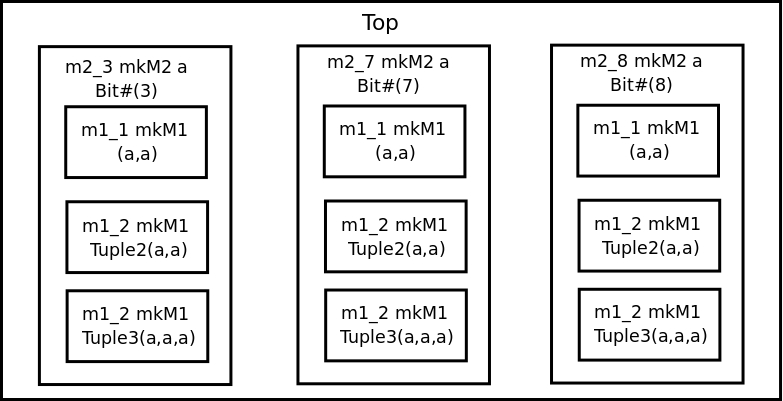
\includegraphics[width = 4 in]{figures/hierarchy}
\caption{Example Module Hierarchy}
\label{hierarchy}
\end{center}
\end{figure}

{\bf Steps for using InstSynth}
 \begin{enumerate}

 \item  Compile your design with bsc as normal, creating the
 \te{.bo} files.

 \item Generate typeclass and default instances for modules with
 the \te{genTypeClass} command, specifying the packages and modules for 
 instance specific synthesis.   The \te{genTypeClass} command will generate
 an include file (\te{<package>}\te{.include.bsv}) for each package.

  The include file will contain  a type class (named
   \te{MakeInst\_<module>}) for each module and a general
   catch-all   instance of that type class.   

   The type class contains one method, which is a module constructor.
   The method is named \te{<module>\_Synth} and has the same arguments as the
   general polymorphic module.  The instance of  this type class is
   a thin wrapper which instantiates the polymorphic module and prints
   a message about the type which is synthesized.

 Example of the include file for \te{m1.bsv} (\te{m1.include.bsv})
 after this step:
 \begin{verbatim}
 typeclass MakeInst_mkM1 #(type ifc_t);
     module mkM1_Synth ( ifc_t ifc) ;
 endtypeclass

 instance MakeInst_mkM1 #(  ClientServer::Server#(a, a) )
     provisos (Bits#(a, sa)) ;

     module mkM1_Synth ( ClientServer::Server#(a, a) ifc) ;
         let _i <- mkM1  ;
         messageM ("No concrete definition of mkM1 for type " +
                    (printType (typeOf (_i))));
         messageM ("Execute: InstSynth::genSpecificInst m1 mkM1 {" +

                     " {" + (printType (typeOf(asIfc (_i)))) + "}" 
                     + " }"  );
         return _i ;
     endmodule
 endinstance
 \end{verbatim}


 \item Manually edit the  \te{.bsv} file to  include the generated file.
 For example, add the line \te{`include "}\te{<package>}\te{.include.bsv"} at the
 bottom of the file for \te{<package>}.  In this example, you would add the line
 \te{`include "m1.include.bsv"} to the file \te{m1.bsv}.

 \item Manually edit the \te{.bsv} file to change the module
 constructor from \te{<module>} to \te{<module\_Synth>} at each point you
 would like an instance synthesized.
 In this example, change  \te{mkM1} to \te{mkM1\_Synth} in the
 \te{m2.bsv} file, and change \te{mkM2} to \te{mkM2\_Synth} in the
 \te{Top.bsv} file where you want to synthesize an instance.


 \item Compile the design again with bsc.   The compile will generate messages
listing missing instances along with the \te{genSpecificInst} command to
 create each missing instance.   Execute the commands 
one at a time to generate an instance for each missing type. 

The \te{genSpecificInst} command will modify the \te{include.bsv} files,
adding the instances.  For example, in this step, the following lines
are added to the \te{m1.include.bsv} file to resolve the
\te{Server\#(a,a)} type.  

\begin{verbatim}
module mkM1__ClientServer_Server_Bit_3_Bit_3_(
                              ClientServer::Server#(Bit#(3), Bit#(3)) ifc ) ;
    let _i <- mkM1  ;
    return _i ;
endmodule

instance MakeInst_mkM1 #( ClientServer::Server#(Bit#(3), Bit#(3)) ) ;
    module mkM1_Synth ( ClientServer::Server#(Bit#(3), Bit#(3)) ifc );
        let _i <- mkM1__ClientServer_Server_Bit_3_Bit_3_  ;
        messageM("Using mkM1__ClientServer_Server_Bit_3_Bit_3_ for mkM1 of
                type: " +
                  (printType (typeOf (_i))));
         return _i ;
     endmodule
endinstance
\end{verbatim}

Note that the code added in this step does not add to or change the
behavior of the design.  Only the additional hierarchy is added.

\item Add provisos to the polymorphic modules to avoid early binding
of the module.  Otherwise compiling at this point will not show the
specific instances because the instance of the \te{\_Synth} is bound
before the specific type of the module is known. In this example,
\te{mkM1\_Synth} would be  bound
before  the specific type of \te{mkM2} is known.  To fix this,  
provisos  are added to the
polymorphic module \te{mkM2}.  The module \te{mkM2} has three
instantiations of \te{mkM1}, therefore a proviso for each
instantiation is  added.

\begin{verbatim}
module mkM2 (Server#(a,a)) provisos (Bits#(a,sa) 
                     ,MakeInst_mkM1#(Server#(a,a))
                     ,MakeInst_mkM1#(Server#(Tuple2#(a,a),Tuple2#(a,a)))
                     ,MakeInst_mkM1#(Server#(Tuple3#(a,a,a),Tuple3#(a,a,a)))
                     );

\end{verbatim} 

\item Compile with bsc again. 

\item Continue  until there are no missing instance messages.   A
Verilog file will be created for each synthesized module instance.

\end{enumerate}


{\bf SynthInst Example Files}
\label{poly-example}

{\bf m1.bsv}: Module \te{mkM1} is defined in the package (file) \te{m1.bsv}:

\begin{verbatim}
   import ClientServer :: *;
   import GetPut :: *;
   import FIFOF :: * ;

   module mkM1 (Server#(a,a))    provisos (Bits#(a,sa));
      FIFOF#(a) fifo <- mkFIFOF;

      interface request = toPut (fifo);
      interface response = toGet (fifo);
   endmodule
\end{verbatim}

{\bf m2.bsv}: Module \te{mkM2} is defined in the package \te{m2.bsv}.  Note that
there are three instantiations of \te{mkM1}.  You can choose to
synthesize any or all of the instances.

\begin{verbatim}
   import FIFO::*;
   import GetPut::*;
   import ClientServer::*;
   import m1 :: *;

   module mkM2 (Server#(a,a))    provisos (Bits#(a,sa)
      Server#(a,a) m1_1 <- mkM1;
      Server#(Tuple2#(a,a),Tuple2#(a,a)) m1_2 <- mkM1;
      Server#(Tuple3#(a,a,a),Tuple3#(a,a,a)) m1_3 <- mkM1;

      rule r0;
         let { x1,x2 } <- m1_2.response.get();
         m1_3.request.put (tuple3 (x1,x2,x2));
      endrule

      interface Put request;
         method Action put (a x);
            m1_2.request.put (tuple2(x,x));
         endmethod
      endinterface

      interface Get response;
         method ActionValue#(a) get ();
            let { y1,y2,y3 } <- m1_3.response.get();
            return (y1);
         endmethod
      endinterface
   endmodule
\end{verbatim}

{\bf Top.bsv}: The testbench is contained in the file \te{Top.bsv}
\begin{verbatim}
   import ClientServer :: *;
   import GetPut :: *;
   import m2 :: *; 
   
   (* synthesize *)
   module mkTb (Empty);
      Reg#(int) cycle <- mkReg (0);
   
      Server#(Bit#(3), Bit#(3)) m2_3 <- mkM2;
      Server#(Bit#(7), Bit#(7)) m2_6 <- mkM2;
      Server#(Bit#(8), Bit#(8)) m2_8 <- mkM2;
   
      rule r1;
         $display ("%0d: r1: put (%0d)", cycle, cycle);
         m2_3.request.put (truncate (pack (cycle)));
         m2_6.request.put (truncate (pack (cycle)));
         cycle <= cycle + 1;
         if (cycle > 8) $finish(0);
      endrule
   
      rule r2;
         let x_3 <- m2_3.response.get ();
         let x_6 <- m2_6.response.get ();
         $display ("%0d: r2: %0d,%0d <= get", cycle, x_3, x_6);
      endrule
   endmodule
\end{verbatim}

% {\bf Example: Using genSynthMod}

% The proc \te{genSynthMod} generates 

% \begin{verbatim}
% import FIFO::*;
% import GetPut::*;
% import ClientServer::*;

% import m1 :: *;
% module mkM2 (Server#(a,a))    provisos (Bits#(a,sa)
%                                         );

%    Server#(a,a) m1_1 <- mkM1;
%    Server#(Tuple2#(a,a),Tuple2#(a,a)) m1_2 <- mkM1;

%    Server#(Tuple3#(a,a,a),Tuple3#(a,a,a)) m1_3 <- mkM1;

%    rule r0;
%       let { x1,x2 } <- m1_2.response.get();
%       m1_3.request.put (tuple3 (x1,x2,x2));
%    endrule

%    interface Put request;
%       method Action put (a x);
%          m1_2.request.put (tuple2(x,x));
%       endmethod
%    endinterface

%    interface Get response;
%       method ActionValue#(a) get ();
%          let { y1,y2,y3 } <- m1_3.response.get();
%          return (y1);
%       endmethod
%    endinterface
% endmodule
% \end{verbatim}

% Given the file m2.bsv, above, and apply \te{genSynthMod}:
% \begin{verbatim}
% genSynthMod m2 mkM2 Server#(a,a) 
% \end{verbatim}

% The result is:

% \begin{verbatim}
% module mkM2__Server_a_a_ ( Server#(a,a) ifc ) ;
%     let _i <- mkM2  ;
%     return _i ;
% endmodule
% \end{verbatim}

% ------------------------------------------------------------

\subsection{Bluetcl Scripts}
Scripts are self-contained commands you run from a shell.  A Tcl
script may be include any combination of Bluetcl and Tcl commands. 

The scripts described in this section are provided with BSC in the
\te{\$BLUESPECDIR/tcllib/bluespec} directory.
To execute a script, type the fully qualified script name.  For
example, to execute the \te{expandPorts} script from a command prompt you would type:
\begin{verbatim}
    $BLUESPECDIR/tcllib/bluespec/expandPorts.tcl
\end{verbatim}

If you are already in a Tcl shell, type  \te{exec} before the script name:
\begin{verbatim}
    exec $BLUESPECDIR/tcllib/bluespec/expandPorts.tcl
\end{verbatim}

% -------------------------

\subsubsection{expandPorts}
\label{script-expandports}

Script to create a Verilog wrapper file which expands structures into
separate Verilog ports.

% -----

\subsubsubsection{Usage:}

{\bf expandPorts.tcl} \{options\} {\em packname} {\em modname}
{\em module.v}

\begin{tabular}{|p {1.8 in}| p {3.8 in}|}
\hline
\hline
options &Optional command line switches: \\
{\bf -p} {\em path}& path, if supplied to the bsc command\\
{\bf -verilog}& compile to verilog (default)\\
{\bf -sim}& compile to bluesim\\
{\bf -include} {\em outfile} &output file for \te{include.vh}\\
{\bf -wrapper} {\em outfile}&output file for \te{wrapper.v}\\
{\bf -rename file.tcl} & Tcl script creating rename pin structure\\
{\bf -makerename}&Create empty \te{.rename.tcl} file to edit for
\te{-rename}\\
{\bf -interface} {\em name}& Interface to expand - defaults to
package name ({\em packname})\\
\hline
{\em packname}& Name of the input \te{.bo} file.\\
\hline
{\em modname} & Name of the top level module.\\
\hline
{\em module.v}& bsc generated Verilog (\te{.v}) file for the module
being wrapped.\\
\hline
\hline
\end{tabular}

% ------------------------------------------------------------
% ------------------------------------------------------------


% ------------------------------------------------------------
% Index

\clearpage
\phantomsection
\addcontentsline{toc}{section}{Index}
\printindex

% ------------------------------------------------------------
% Appendix: Commands by Namespace

\clearpage
\phantomsection
\addcontentsline{toc}{section}{Commands by Namespace}
\printindex[commands]

% ------------------------------------------------------------

\end{document}
